\title{Group 26 Report: Rotten Potatoes} % Title
\author{郑时飞 \\ 朱伯源 \\ 李易 \\ 汪明杰 \\ 施天昊}% Author
\date{\today}% Date

\documentclass[11pt]{article}
\usepackage[margin=1in]{geometry}
\usepackage{vmargin}
\usepackage{url}
\usepackage{datetime}
\usepackage[utf8]{inputenc}
\usepackage{CJKutf8}
\usepackage{graphicx}
\usepackage{mathtools}
\usepackage{float}
\usepackage[colorlinks,linkcolor=blue,urlcolor=blue]{hyperref}


\makeatletter 
    \newcommand\fcaption{\def\@captype{table}\caption}
\makeatother
\setmarginsrb{3 cm}{2.5 cm}{3 cm}{2.5 cm}{1 cm}{1.5 cm}{1 cm}{1.5 cm}

\makeatletter
\let\thetitle\@title
\let\theauthor\@author
\let\thedate\@date
\makeatother

\usepackage{graphicx, bm}
\graphicspath{{graphics/}}
\usepackage{geometry}
\geometry{left=5cm,top=5cm,right=0cm,bottom=0cm}

\usepackage[colorlinks,linkcolor=blue]{hyperref}

\begin{document}
\begin{CJK*}{UTF8}{gbsn}

\begin{titlepage}
    \centering
    \vspace*{0.5 cm}
    
\includegraphics[scale = 0.75,width=6cm]{CUHK}\\[1.0 cm]
    \textsc{\large The Chinese University of Hong Kong, Shenzhen}\\[1.5 cm] 
    \textsc{\Large CSC 3170}\\[0.5 cm] 
    \textsc{\large Database System}\\[0.5 cm]
    \rule{\linewidth}{0.2 mm} \\[0.4 cm]
    { \huge \bfseries \thetitle}\\
    \rule{\linewidth}{0.2 mm} \\[0.6 cm]
    
    \begin{minipage}{0.4\textwidth}
        \begin{flushleft} \large
            \emph{Authors:}\\
            郑时飞 \\ 朱伯源 \\ 李易 \\ 施天昊 \\ 汪明杰
            \end{flushleft}
    \end{minipage}~
    \begin{minipage}{0.4\textwidth}
            \begin{flushright} \large
            \emph{Student Number:} \\
            119010465 \\ 119010485 \\ 119010156 \\ 120090472 \\ 119010300
        \end{flushright}
    \end{minipage}\\[2 cm]
    {\large \thedate}\\[2 cm]
 
    \vfill
    
\end{titlepage}

\tableofcontents
\pagebreak

\rmfamily
\section{Introduction}
\paragraph{}As an art and commercial work, movies have become pursuits of many people and generated tremendous value. Currently, there are two types of online movie platforms. On the one hand, platforms including Rotten Tomatoes and Douban gives people rich information regarding movies. On the other hand, sites like Netflix offers precise, personalized recommendation to users. Such a recommendation strategy allows users to discover more films they enjoy and attracts more users to the platform.
\paragraph{}However, currently, no site combines the strengths of the mentioned movie sites. Besides, existing popular movie websites are full of quarrels and controversies from the perspective of the community environment. The movie recommendations are influenced deeply by the advertising, not the quality of films. Therefore, to satisfy the real requirements of movie lovers, we built a movie database called \textbf{\href{http://10.20.9.99:3000}{Rotten Potatoes}}, based on which, users can talk about their reviews of the movie freely. It also offers plenty of searching functions and personalized recommendations from the platform. 
\paragraph{}We use python packages \textbf{\href{https://docs.python-requests.org/en/latest/}{Requests}} and \textbf{\href{https://www.crummy.com/software/BeautifulSoup/bs4/doc/}{BeautifulSoup}} to obtain the required data from IMDB, store it in a MySQL database. Then we build our searching functions and personalized movie recommendations on those data. We also build a user-friendly web using \textbf{\href{https://aisuda.bce.baidu.com/amis/zh-CN/docs/index}{amis}} as the frontend and \textbf{\href{https://expressjs.com}{express}} as the backend.
\section{Design}
In this section, we focus on the design of the Entity-Relationship Model, 
the reduction from ER diagram into relational schemas, constraints and index.

\subsection{Entity-Relationship Model}
As shown in the \hyperref[ERD]{ER diagram}, there are 5 entities and 3 relationships. 
\subsubsection{Entities}
\begin{itemize}
\item \textbf{Entity ``crew''} The crew participating in shooting movies. Each crew has identifying id, name, photo URL, introduction and birth date. The entity ``crew'' is a generalization of entity ``directors'' and ``actors''.
\begin{itemize}
\item \textbf{Entity ``directors''} The directors that direct movies. A specification of entity ``crew''. Each director has the same attributes as the crew. 
\item \textbf{Entity ``actors''} The actors that act in movies. A specification of entity ``crew''. Each actor has the same attributes as the crew. 
\end{itemize}
\item \textbf{Entity ``users''} The users of our movie website. Each user has identifying id, name, avatar URL and password. 
\item \textbf{Entity ``movies''} The movie information. Each movie has identifying id, name, cover URL, introduction, release year and genres, where genres is a multivalued attribute.
\end{itemize}
\subsubsection{Relationships}
\begin{itemize}
\item \textbf{Relationship ``direct''} Directors direct movies. A many-to-one relationship between entity ``movies'' and ``directors'', which means a director can direct multiple movies while a movie can only be directed by one director, in our assumption. 
\item \textbf{Relationship ``act''} Actors act in movies. A many-to-many relationship between entity ``movies'' and ``actors''. An actor acts in a movie as a character with an attribute character name. 
\item \textbf{Relationship ``comment''} Users comment movies. A many-to-many relationship between entity ``movies'' and ``users''. A user comments a movie by a comment with attributes comment date, rate and content. 
\end{itemize}

\begin{figure}[h]
\centering
\label{ERD}
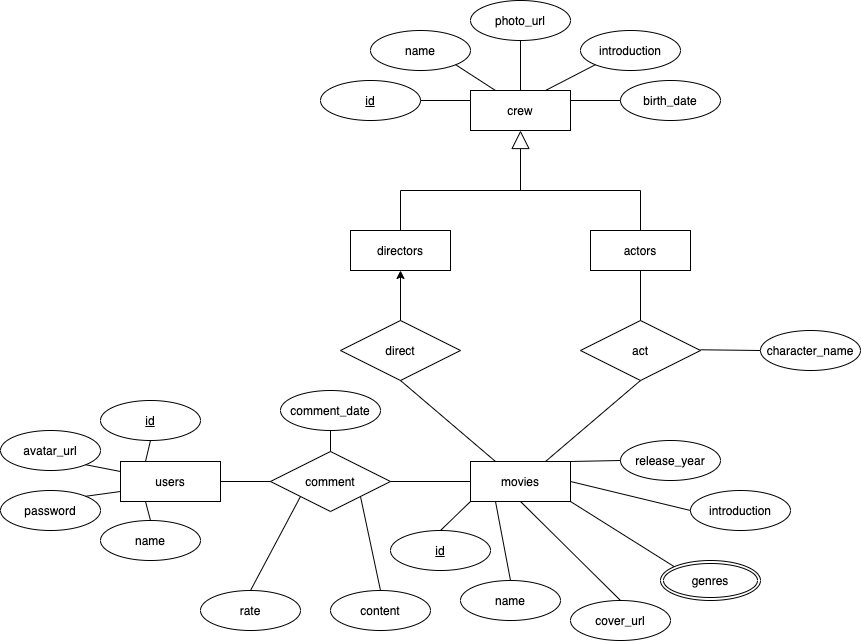
\includegraphics[width=0.5\textwidth]{er.png}
\caption{ER Diagram}
\end{figure}

\subsection{Relational Schema}
As shown in the \hyperref[RelationalSchema]{relational schema diagram}, there are 7 schemas. \\\\
The following reductions are made:
\begin{itemize}
\item The attribute ``genres'' in entity ``movies'' is reduced to schema ``genres'' with attributes ``genres\_name'' and ``movie\_id'' as a foreign key referencing ``id'' of ``movies''. Both of the attributes form a primary key to make sure no redundant genres in a movie.
\item The relationship ``direct'' is reduced to attribute ``director\_id'' as a foreign key referencing ``movies'' for the many-to-one relationship. 
\item The relationship ``act'' is reduced to schema ``characters''. Except for attribute ``character\_name'', extra attributes ``movie\_id'' as a foreign key referencing ``movies'' and ``actor\_id'' as a foreign key referencing ``actors'' are added for the many-to-many relationship. Attribute ``id'' is also added to allow an actor to act as multiple characters in the same movie. 
\item The relationship ``comment'' is reduced to schema ``comments''. Except for attributes ``comment\_date'', ``rate'' and ``content'', extra attributes ``movie\_id'' as a foreign key referencing ``movies'' and ``user\_id'' as a foreign key referencing ``users'' are added for the many-to-many relationship. Attribute ``id'' is also added to allow a user to make multiple comments on the same movies. 
\item All identifying ``id''s are reduced to the primary keys. 
\end{itemize}

\begin{figure}[h]
\centering
\label{RelationalSchema}
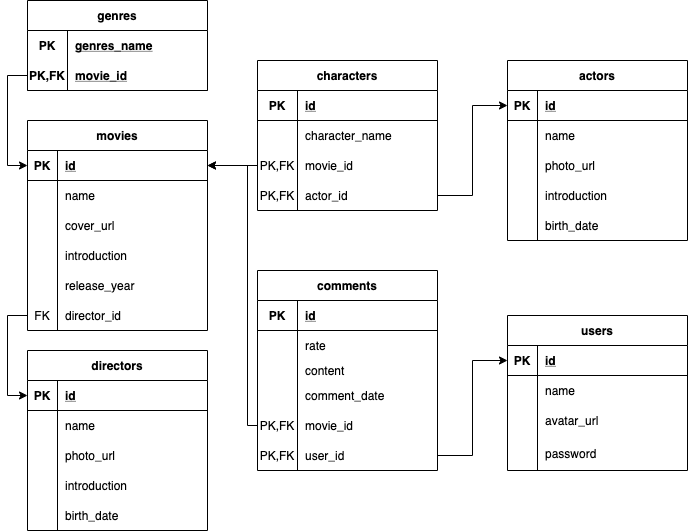
\includegraphics[width=0.6\textwidth]{schema.png}
\caption{Relational Schema Diagram}
\end{figure}

\subsection{Constraint}
3 types of constraints are further added:
\paragraph{Not Null Constraints}
\begin{itemize}
\item All ``id'' attributes as they are primary key and thus automatically becoming not null.
\item ``name'' attribute of schema ``movies''.
\item ``name'' and ``director\_id'' attributes of schema ``directors'', as a movie is directed by exactly one director.
\item ``name'' attribute of schema ``actors''.
\item ``name'' and ``password'' attributes of schema ``users''.
\item ``actor\_id'', ``movie\_id'' and ``character\_name'' attributes of schema ``characters'', as it is a weak entity of schemas ``actors'' and ``movies''.
\item ``user\_id'', ``movie\_id'', ``rate'', ``content'' and ``comment\_date'' attributes of schema ``comments'', as it is a weak entity of schemas ``users'' and ``movies''.
\item ``genres\_name'', ``movie\_id'' attributes of schema ``genres'', as it is a multivariate attribute of schema ``movies''.
\end{itemize}
\paragraph{Unique Constraint}
A unique constraint is added to the ``name'' attribute of schema ``users'' as by our assumption there should be no repeating user names. 
\paragraph{Check Constraint}
A check constraint is added to the ``rate'' attribute of schema ``comments'' to make sure the rate is from 0 to 10.

\subsection{Index}
The following attributes are indexed to make searching faster:
\begin{itemize}
\item ``name'' and ``release\_year'' attributes of schema ``movies''.
\item ``name'' and ``birth\_date'' attributes of schema ``directors''.
\item ``name'' and ``birth\_date'' attributes of schema ``actors''.
\item ``name'' attribute of schema ``users''.
\end{itemize}

\section{Implementation}
In this section, we will introduce the implementation of our movie website. All codes of this project can be accessed from \href{https://github.com/warin2020/rotten-potatoes}{https://github.com/warin2020/rotten-potatoes}.
\subsection{Frontend}
The frontend of our project is constructed using \textbf{\textit{\href{https://aisuda.bce.baidu.com/amis/zh-CN/docs/index}{amis}}}, a low-code frontend framework. It can generate a website using JSON configurations, which is suitable for developing a lightweight and agile application like this project. We constructed the following pages:
\begin{itemize}
    \item Movie: a list of all the movies with their name and posters. Each movie is a "Card" widget linking to the movie detail page.
    \item Actor: a list of all the actors/actresses, also implemented using the "Card" widget, containing links to the detailed information.
    \item Director: a list of all the directors implemented similarly to the \textbf{Actor} page
    \item Comment: this page contains the latest comments that users release.
    \item Me: a portal for users to edit their information. Including updating avatar, name and password. This page also contains a list of movies recommended to the user.
    \item Search: to search for movies/actors/users, we implemented three different pages. The details will be discussed in the \textbf{Sample Queries} section.
\end{itemize}
\par Since our application is user-oriented, the UI of our website is very concise and user-friendly. Screenshots of our UI can be found in the appendix.


\subsection{Backend}
\paragraph{Connect to MySQL in Nodejs}
The query functions in our database are written in javascript language. They can be found in the corresponding files in the \textbf{services} folder. To maximize reusability, we wrote a template query function in \textbf{query.js} using the \textit{mysql} module of Node.JS. The template function will first access the \textbf{.env} file for database configuration(e.g., the port on which the MySQL server is running, the logging username and password). Then, instead of establishing and closing connections to the database on every execution, the template creates a connection pool. Requests from the frontend will pass the query as a rest parameter to the template function, which will then issue the query and return the results (and errors, if any) back to the frontend.
\paragraph{Provide API by Express Router}
We use the \textbf{\href{https://expressjs.com}{express}} library to provide APIs for frontend users. All the routers are written in the \textbf{router/index.js}. Whenever users access a certain page, it will match a router in the file, which triggers the corresponding handler function. For example, after logging in, the user will see the \textit{Movie} page, which contains a list of movies in the database. When the user clicks on any of the movie poser, the frontend will request for page \underline{./movie/detail/$<$movie\_id$>$}, matching a router in index.js (line 26). The router then calls the corresponding handler function, in this case, the \textit{getMovieDetail()} function in \textbf{movie.js}, which directs the user to the corresponding movie detail page.
\begin{figure}[h]
    \centering
    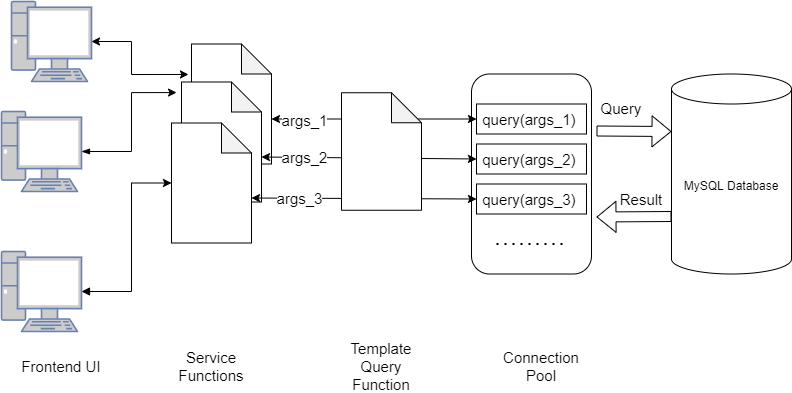
\includegraphics[width=0.4\textwidth]{sqlconnect.png}
    \caption{Database connection flowchart}
\end{figure}
\paragraph{Access Control by jsonwebtoken}
\label{sec:access}
Based on \textbf{\href{https://www.npmjs.com/package/jsonwebtoken}{jsonwebtoken}} package, in \textbf{auth/auth.js} using the key in \textbf{.env} file \textbf{SECRET\_KEY} we implemented 2 functions \textit{signToken} and \textit{verifyToken}, by which, in \textbf{services/auth.js}, the routing function \textit{login} returns a token to frontend and the middleware function \textit{auth} checks whether the token from frontend is correct and not outdated.

\subsection{Web Crawler}
\subsubsection{Basic Workflow}
To populate our database with real-world data, we wrote a web crawler to scrap information from IMDB's Top 250 Movie Chart. The crawler is written in Python. It uses the \textbf{\href{https://docs.python-requests.org/en/latest/}{Requests}} library to send HTTPS requests. The desired fields are acquired through parsing the page using \textbf{\href{https://www.crummy.com/software/BeautifulSoup/bs4/doc/}{BeautifulSoup}} library.
The detailed process is shown in this \hyperref[crawler]{flowchart}:\par

\begin{enumerate}
    \item Access the Top 250 Chart, where all the URLs to the detailed movie pages are located
    \item Traverse through the chart. For every movie on the chart:
    \begin{enumerate}
        \item Access the detailed movie page, where information regarding the movie can be found.
        \item From the detailed movie page, we access the casting information.\\ For the director:
        \begin{itemize}
            \item For directors yet to be recorded, access the detailed director page, where information regarding the director can be found.
        \end{itemize}
        For the actors/actresses who cast in this movie:
        \begin{itemize}
            \item Access the detailed actor/actress page and find detailed information if their details are yet to be recorded.
        \end{itemize}
        \item The comment section locates at the bottom of the movie page. We collect the rating, comments from this section.
        \item For each comment, we acquire the user information by accessing their homepage.
    \end{enumerate}
\end{enumerate}

\begin{figure}[h]
    \label{crawler}
    \centering
    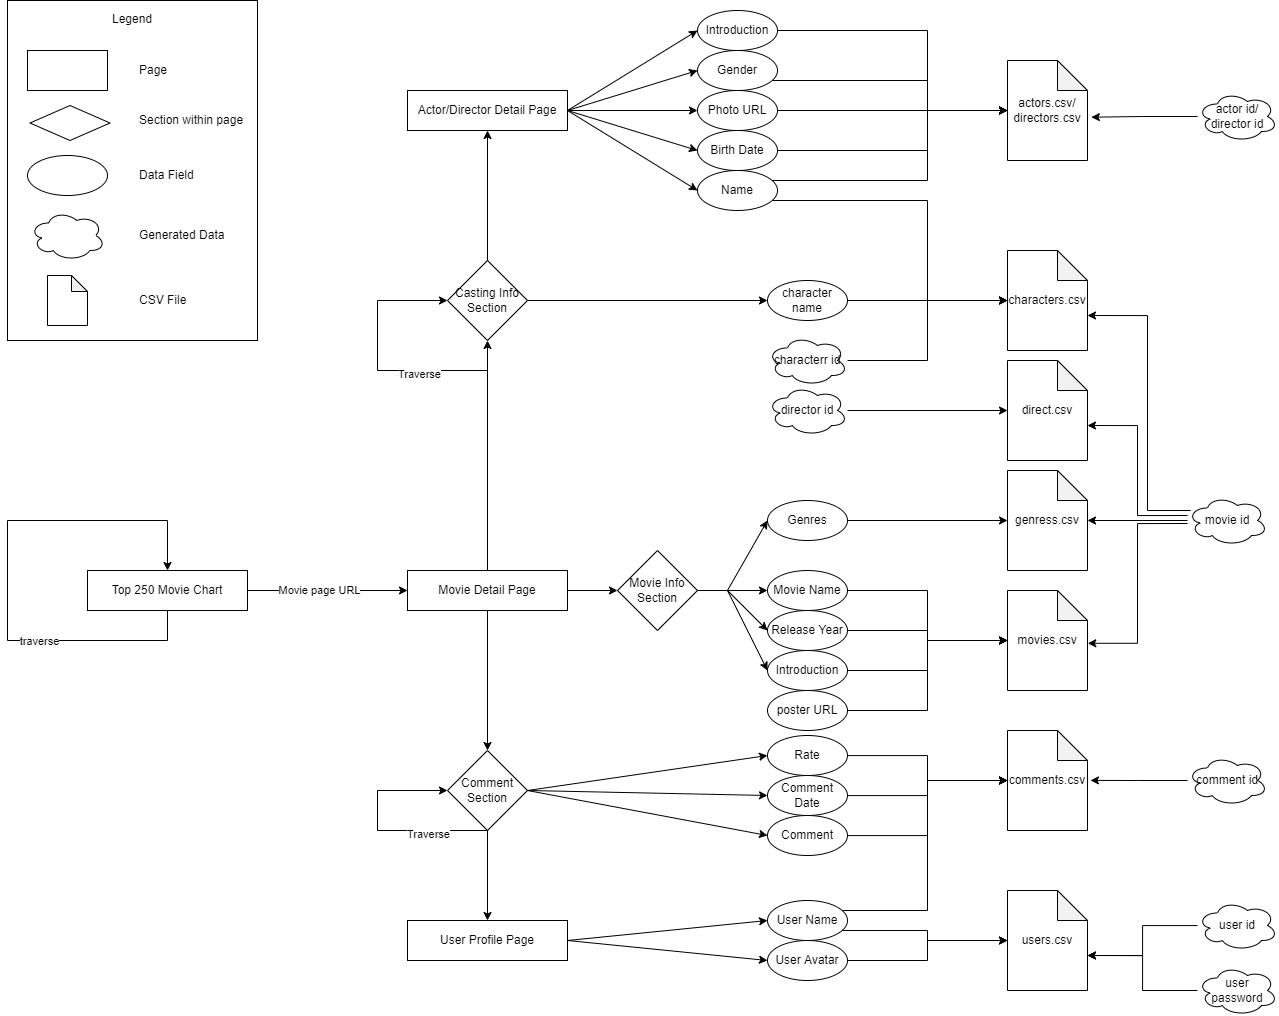
\includegraphics[width=0.4\textwidth]{crawler_flowchart.png}
    \caption{Web crawler flowchart}
\end{figure}

\subsubsection{Encountered Problems and Solutions}
During the scrapping process, we encountered some issues.
\begin{itemize}
    \item The same director or actor/actress can participate in different movies. Therefore, we keep a mapping relationship and check whether we have recorded the same person's information. This step is done through hashing the person's name, which takes O(1) complexity.
    \item We do not have access to each user's password, so we randomly generate a password for each user we scrapped from IMDB. The password is a random combination of 5 to 10 numbers and characters.
    \item Some actors' birth dates cannot be achieved from their detailed page. We leave them as NULL.
    \item The gender of the movie stars is not explicitly listed on their detail page. However, by seeking their role in the movie (i.e, actor/actress), we can acquire their gender.
\end{itemize}
\subsection{Sample Queries}
\subsubsection{User account \& the Portal}
\paragraph{User registration}
When a user tries to create his own account, he needs to specify his user name. In our system, every user must have a unique account name. Therefore, before granting a registration, we will first query the inputted user name in the \textbf{users} table. If the name already exists, the registration will not be accepted and the user should input a new user name. Otherwise, the user name, as well as user password, will be inserted into the user table, with a user ID generated automatically.






\paragraph{User login}
When a user log in, password will be queried from the user table, with the user name as the search key. Then, the correct password will be checked using jsonwebtoken, as mentioned in the \hyperref[sec:access]{access control section}

\begin{figure}[htbp]
    \centering
    \begin{minipage}[t]{0.32\textwidth}
    \centering
    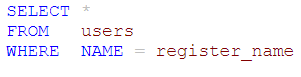
\includegraphics[width=6cm]{reg_ver.png}
    \caption{User registration verification}
    \end{minipage}
    \begin{minipage}[t]{0.32\textwidth}
    \centering
    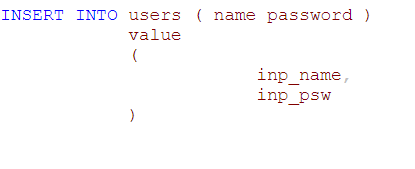
\includegraphics[width=6cm]{reg_ins.png}
    \caption{User registration verification insert}
    \end{minipage}
    \begin{minipage}[t]{0.32\textwidth}
    \centering
    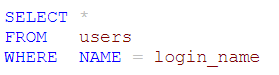
\includegraphics[width=6cm]{login.png}
    \caption{User login}
    \end{minipage}  
\end{figure}

\paragraph{The Portal}
User can modify his avatar, user name and password. This is achieved by updating a record in the \textbf{users} table.
\begin{figure}[htbp]
\centering
\begin{minipage}{0.32\textwidth}
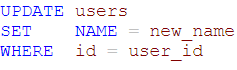
\includegraphics[width=\linewidth]{avatar.png}
\caption{Update avatar}
\end{minipage}
\begin{minipage}{0.32\textwidth}
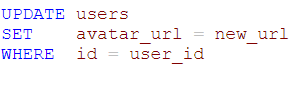
\includegraphics[width=\linewidth]{name.png}
\caption{Update user name}
\end{minipage}
\begin{minipage}{0.32\textwidth}
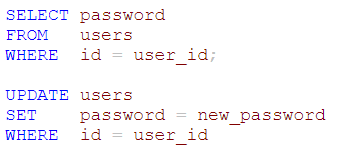
\includegraphics[width=\linewidth]{password.png}
\caption{Update user password}
\end{minipage}
\end{figure}

\paragraph{Delete user}
In our system, a user account can be deleted, while the comments on movies he made will be kept even after the account is deleted. This is achieved by associating the comments to a padding user before deleting the user account.
\begin{figure}[!htb]
    \centering
    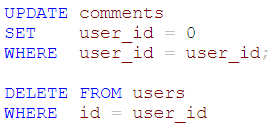
\includegraphics[width=0.3\textwidth]{user_del.png}
    \caption{Delete user}
\end{figure}


\subsubsection{CRUD on movies, actors and directors}
\paragraph{Information listing}Movies, actors and directors are listed on our web page. Basic information is selected from the corresponding table.
\begin{figure}[htbp]
\centering
\begin{minipage}{0.32\textwidth}
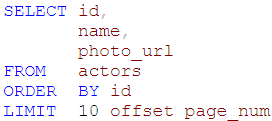
\includegraphics[width=\linewidth]{a_list.png}
\caption{Listing actor}
\end{minipage}
\begin{minipage}{0.32\textwidth}
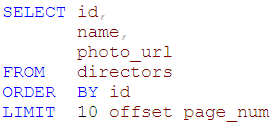
\includegraphics[width=\linewidth]{dir_list.png}
\caption{Listing directors}
\end{minipage}
\begin{minipage}{0.32\textwidth}
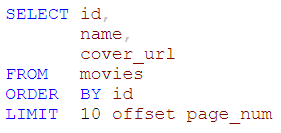
\includegraphics[width=\linewidth]{m_list.png}
\caption{Listing movies}
\end{minipage}
\end{figure}

\paragraph{Detail information} To show detailed information	 movies, actors and directors, we need to join several tables. \textbf{Actors} table is joined with the \textbf{characters} table to get all characters played by an actor, while \textbf{directors} table is joined with \textbf{movies} table to select all movies directed by the director. For the detail page of movies, 4 table joins are needed to acquire all necessary data. \textbf{Movies} table is joined with \textbf{characters} table to get all characters in a specific movie. Joining the \textbf{directors} table is also necessary to find the director of a specific movie. All comments and genres of the movie are obtained by joining the \textbf{movies} table with the \textbf{comments} table and \textbf{genres} table, respectively. Figure 16 displays the query used to generate actor details:

\begin{figure}[htbp]
\centering
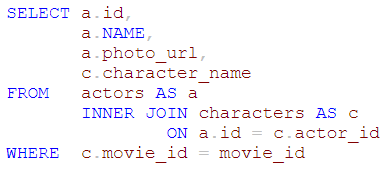
\includegraphics[width=6cm]{a_detail.png}
\caption{Actor detail}
\end{figure}

\paragraph{Search movies}
Movies can be searched using their names. Aside from directly searching, we also support filtering movies by their release time, movie rate and movie genres. We also added support for ordering (in ascending or descending order) the result by name, release year and rating.
\begin{figure}[htbp]
\centering
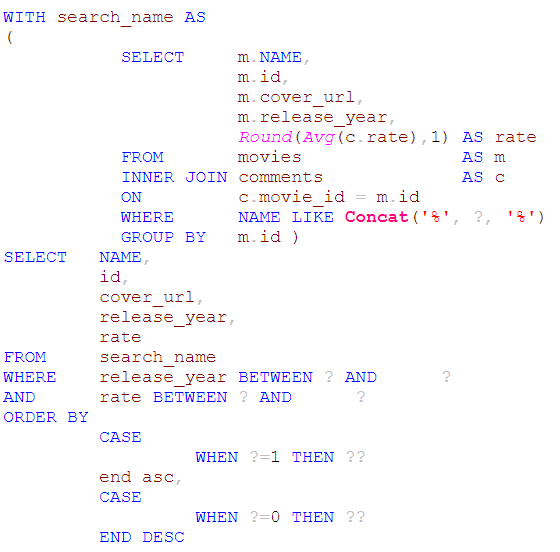
\includegraphics[width=0.4\textwidth]{m_search.png}
\caption{Movies search}
\end{figure}
\paragraph{Search actors}
Similar to movies, actors are searched by their name, and filtered by their birth date. Also, ordering is supported on the birth date and name.
\paragraph{Search user}
For user searching, only name search is supported.


\subsubsection{Comments}
\paragraph{List comments}
Join the \textbf{comments} table and the \textbf{users} table to match the sender of each comment. After joining, all tuples are shown. 
\begin{figure}[h]
    \centering
    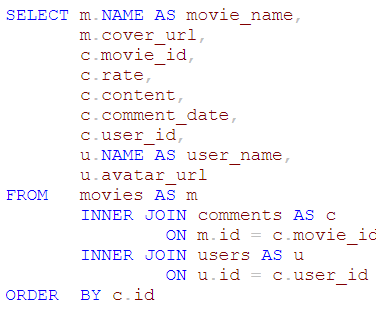
\includegraphics[width=0.4\textwidth]{comment.png}
    \caption{Comments list}
\end{figure}
\paragraph{Delete comments} 
Comments deletion is achieved by deleting the corresponding tuples comment table.
\paragraph{Add comments} 
Comment addition is achieved by inserting it into the comment table.

\subsection{Data Analysis}
\subsubsection{Recommendation System with Restricted Boltzmann Machines}

In 2007, Hinton showed that Restricted Boltzmann Machines (RBMs) can be successfully applied to the Netflix dataset and do personalized movie recommendations (Hinton et al., 2007). This paper was given in a DDA course project, but that project requires only the basic RBM without biases, conditional RBM and neighborhood. We reproduce \hyperref[RBM]{the model proposed by Hinton} in this project to do recommendations. We use Contrastive Divergence (CD) to approximate the maximum likelihood of the parameters by Gibbs sampling. The notions for the following procedure can be found in \href{rbm}{the model}.
\begin{enumerate}
    \item Acquire the visible movie ratings $ \bm{V} $ of the user, each $ \bm{v} $ is $ K $ binary vector where $ \bm{v}^k = 1 $ if the rating is $ k $, otherwise 0.
    \item Sample the hidden units $ \bm{h} $ to binary numbers by probability given by \\ $ p(h_j = 1 | \bm{V}, \bm{r}) = \sigma(c_j + \sum_{i = 1}^m \sum_{k = 1}^K v_i^k W_{ij}^k + \sum_{i = 1}^M r_i D_{ij}) $, where $ \sigma(x) = \frac{1}{1 + e^{-x}}  $.
    \item Reconstruct the visible units by $ p(v_i^k = 1 | \bm{h}) = softmax(b_i^k + \sum_{j = 1}^F h_j W_{ij}^k) $, \\where $ softmax(x_k) = \frac{e^{x_k}}{\sum_{l= 1}^K e^{x_l}} $. Notice that we only reconstruct the movies the use has rated.
    \item Update the parameters by the origin data and reconstructed data. For example, $ \Delta W_{ij}^k = \epsilon (<v_i^k h_j>_{data} - <v_i^k h_j>_T) $, where $ T $ represents the number of runs we do Gibbs sampling.
    \item Prediction is much the same as doing Gibbs sampling except that we can reconstruct (predict) missing ratings.
\end{enumerate}

\begin{figure}[htbp]
\centering
\label{RBM}
\begin{minipage}[t]{0.45\textwidth}
\centering
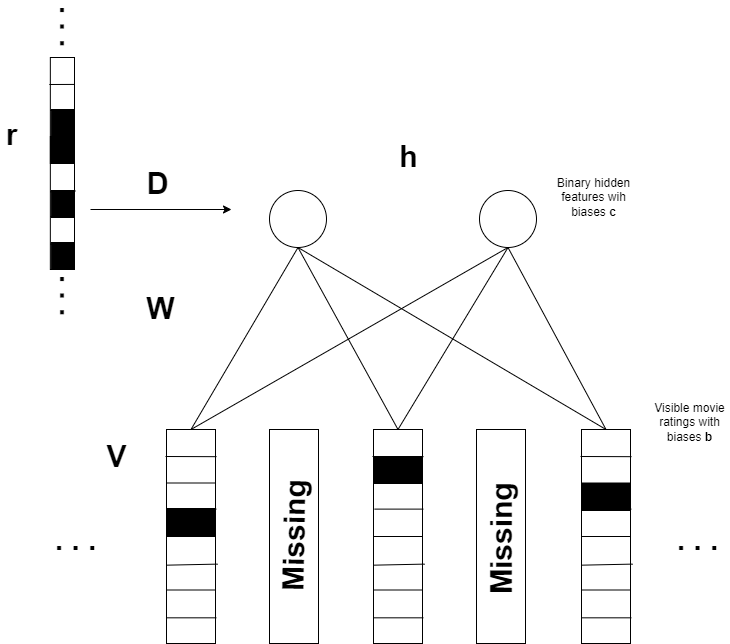
\includegraphics[width=6cm]{conditionalRBM.png}
\caption{Conditional RBM}
\label{rbm}
\end{minipage}
\begin{minipage}[t]{0.45\textwidth}
\centering
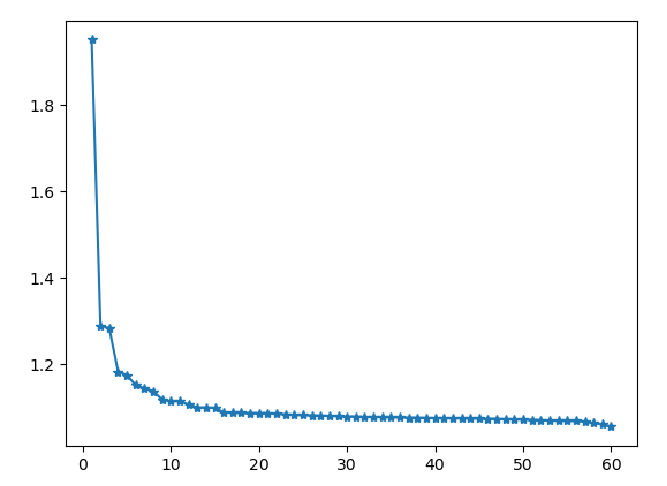
\includegraphics[width=6cm]{RBMResult.png}
\caption{Train RMSE vs. Epochs}
\end{minipage}
\end{figure}

\hyperref[RBM]{Figure above} shows the evolution of Root Mean Squared Error (RMSE) during training. We achieve an RMSE of 1.04. Every time the user enters the \textbf{Me} page on our website, the system will automatically predict the ratings overall movies and recommend the top 8 movies to the user in \textbf{Guess you like} module. An example on the webpage is shown in \hyperref[recommend]{figure below}.

\begin{figure}[h]
    \centering
    \label{recommend}
    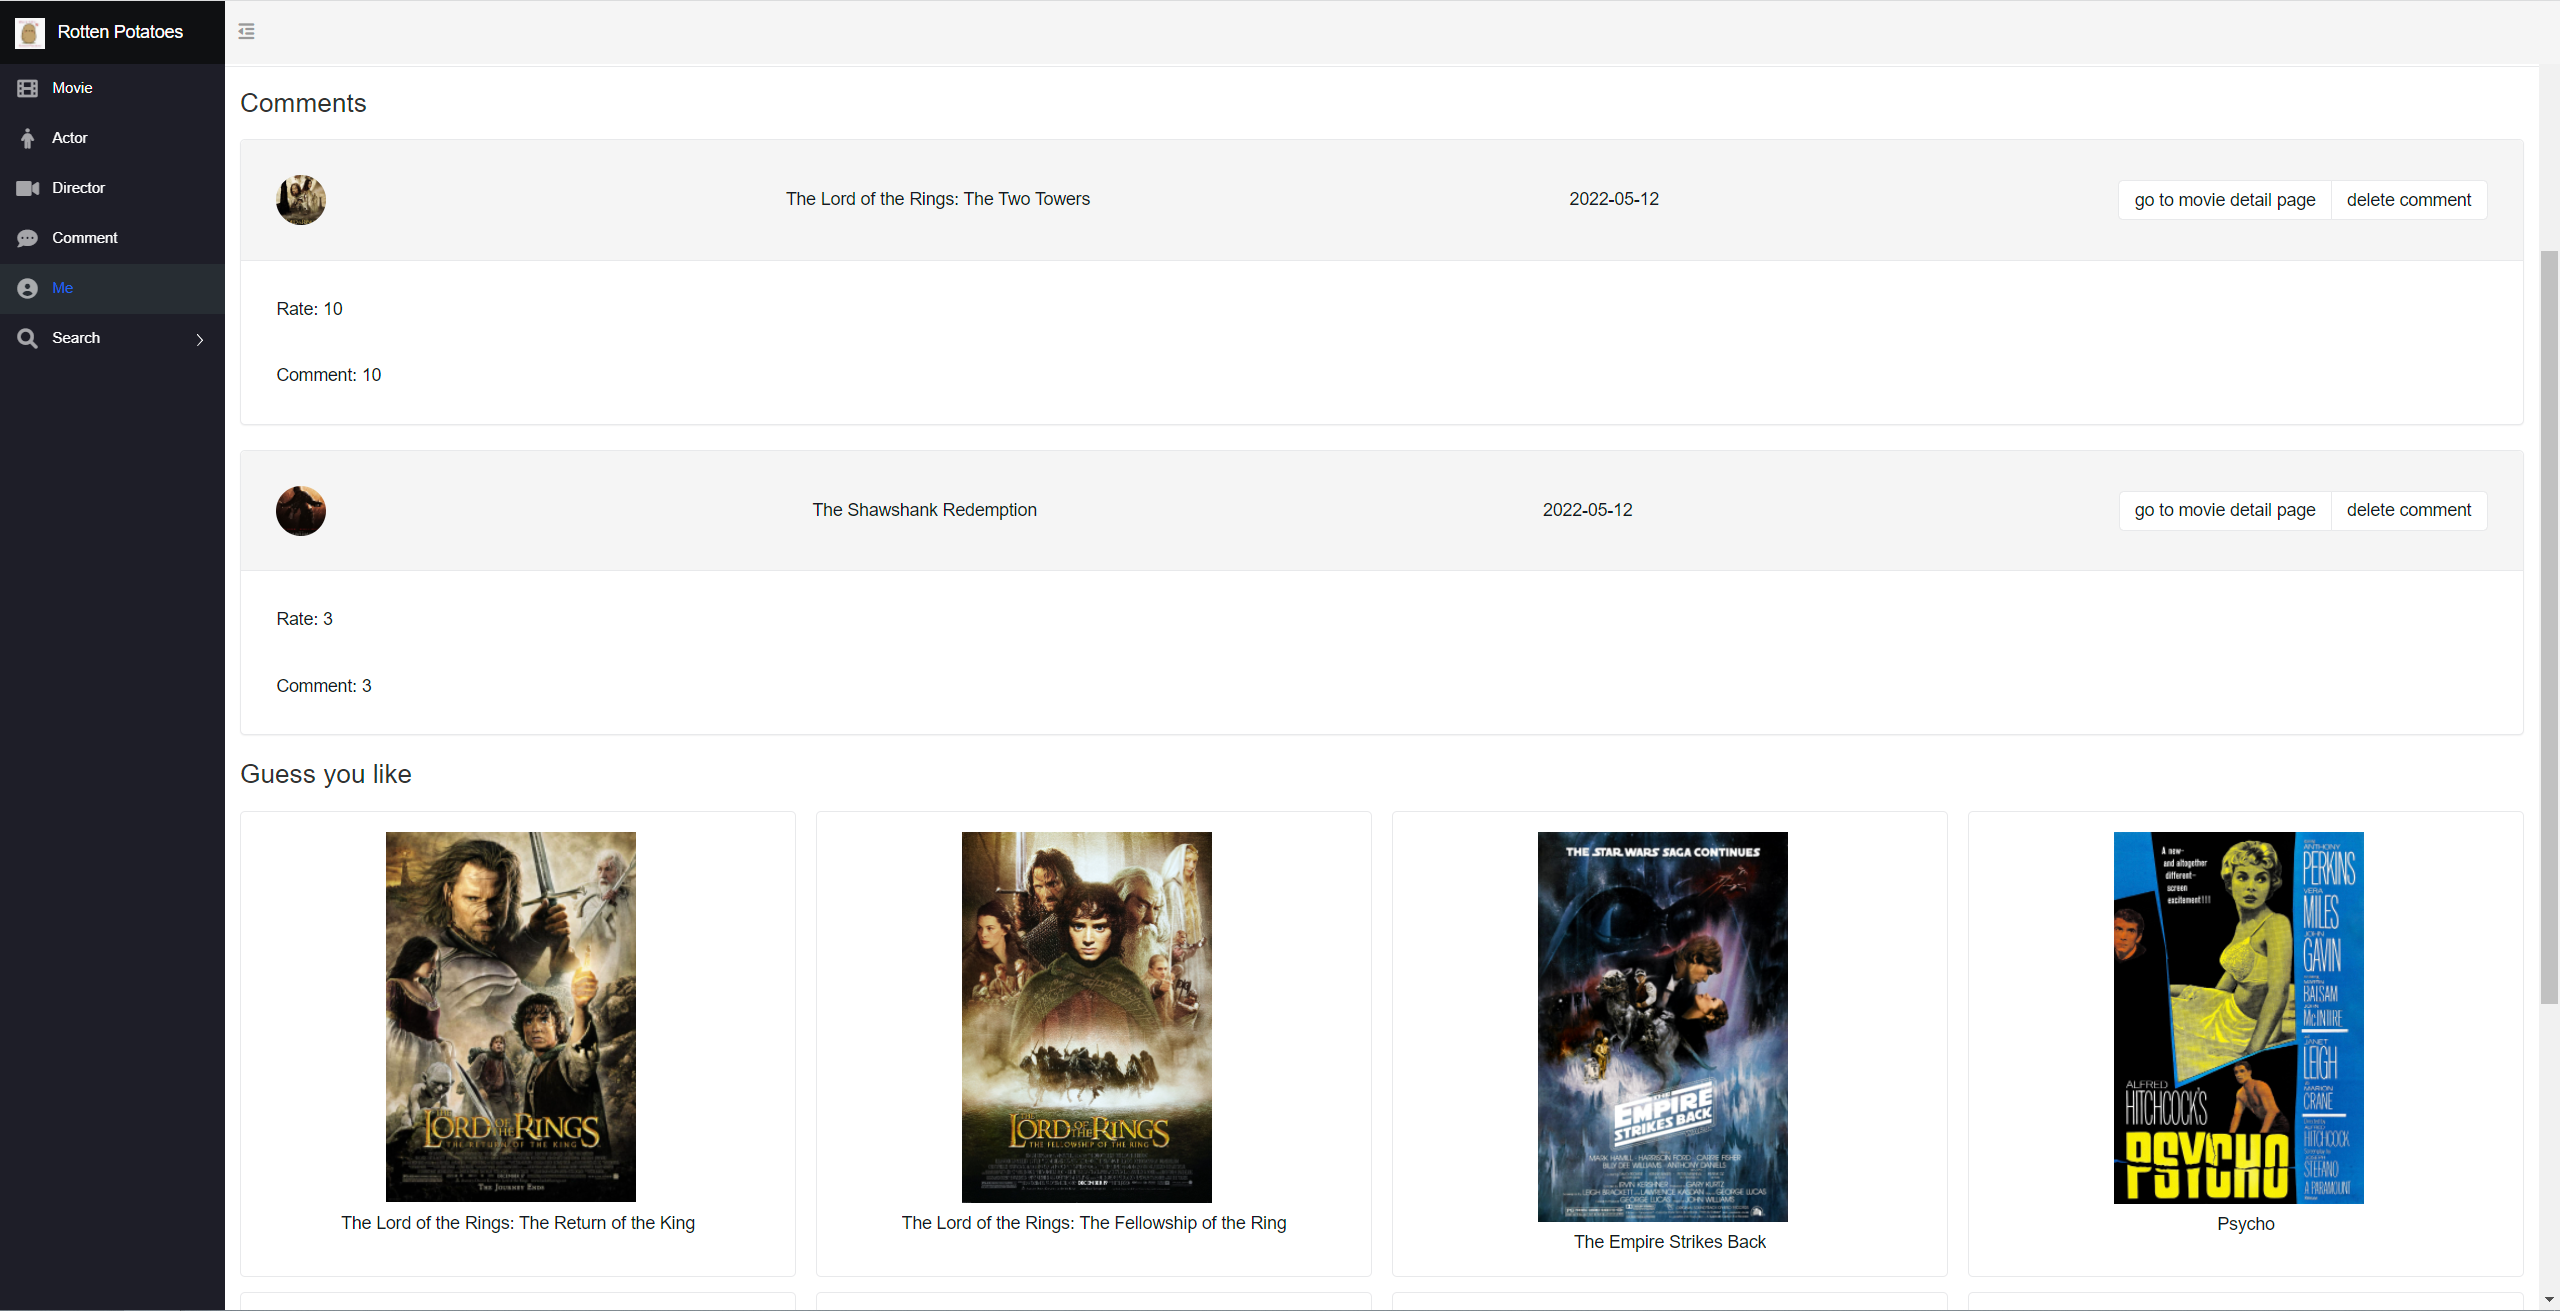
\includegraphics[width = 0.55\textwidth]{recommendation.png}
    \caption{Personalized Movie Recommendation}
\end{figure}

\subsubsection{Neighbourhood Model}
Users have their preferences and tend to give similar ratings to movies of the same kind. In other words, movies are correlated and we can utilize this property to improve our predictions $ \hat{R} $ :
\begin{itemize}
    \item Define an error matrix by $ \widetilde{R} = R - \hat{R} $
    \item Define similarity between two movies by their column features (user ratings): $ d_{A B}=\frac{\tilde{r}_{A}^{T} \widetilde{r}_{B}}{\left\|\widetilde{r}_{A}\right\|_{2}\left\|\widetilde{r}_{B}\right\|_{2}} $
    \item Predict the error of one movie through the errors of its neighbours: $ \hat{\tilde{r}}_{i A}=\frac{1}{\sum_{B \in S}\left|d_{A B}\right|} \sum_{B \in S} d_{A B} \widetilde{r}_{i B}  $, where $ S $ is the set of neighbours (with high absolute similarities) of $ A $.
    \item Improve our RBM predictions by $ R_{u m}^{*}=\hat{R}_{u m}+\hat{\tilde{r}}_{u m} $ for each $ (user, movie) $ pair desired.
\end{itemize}
We improve the RMSE from 1.04 to 1.02. The improvement is not high because our matrix is sparse. In our data set, many users only give one rating, so it is hard to construct a well defined similarity matrix. The other reason is that we crawl high-rating movies and the biases are not large to give a performance boost. However, we are still able to leverage the data and get some insight into the movie ratings. \\\\
For example, \textit{The Godfather: part II} has a high similarity($ 0.9999 $) with \textit{The Godfather}(based on the difference between real rating and predicted rating), which is expected. However, the similarity between \textit{The Godfather} and the two sequels of \textit{The Lord of the Rings} diverge. \textit{The Fellowship of the Ring} has a similarity of $ 0.9999 $ with \textit{The Godfather}, while its sequel \textit{The Return of the King } has a similarity of $-0.9999 $. This is counterintuitive and we should look into the data. We have three users giving ratings to both \textit{The Godfather} and \textit{The Lord of the Rings: The Return of the King}. The ratings are $ (10, 10) $, $ (10, 10) $ and $ (8, 10) $, respectively. For \textit{The Godfather} and \textit{The Lord of the Rings: The Fellowship of the Ring}, the rating pairs are all $ (10, 10) $. A rating of 8 is a relatively low rating in our dataset, hence the algorithm concludes that they are negatively correlated.

\section{Result}
The website can be accessed through URL \href{http://10.20.9.99:3000}{http://10.20.9.99:3000}. This server can only be accessed within the CUHK(SZ) campus network. In case of access failure, please contact our group member Tianhao SHI (120090472), who is in charge of server maintenance. You can also find the source code on our \href{https://github.com/warin2020/rotten-potatoes}{Github repository}. Snapshots of our website can be found in the appendix.
\section{Conclusion}
\paragraph{} In this project, we build a movie database based on large-scale data collected from \textbf{IMDB}. Additional attention is paid to assure a \textbf{BCNF} form is kept for every schema in our database, thus the redundancy part is eliminated. We also \textbf{implement useful functions} for our users to search for the movies, casts or other users using name,  time information, rate(only movies) and genres(only movies) as the keyword.
\paragraph{}To improve user experience and replace the complex database operations with a few simple mouse clicks from users, we build a user-friendly website. Based on that, abundant \textbf{personalized interaction behaviors} can be achieved, which serves our users more conveniently. We hold an integral process of account management for users. Users can add comments to a movie and rate it as well as discover their appreciated reviews or users.
\paragraph{} It is common for a movie database to recommend movies that the users have a potential interest in. However, how to make a personalized recommendation list of high quality is always a problem. We use a lot of techniques in the data analysis to satisfy the needs of users. We build a \textbf{Restricted Boltzmann Machines}  with \textbf{Neighbourhood model} and get gratifying results.
\section{Self Evaluation}
In this part, we evaluate the advantages and disadvantages of our project.
\subsection{What we have achieved}
\begin{itemize}
\item Build a database conforming to the low redundancy paradigm
\item Implement and optimize many necessary  searching functions
\item Create a user-friendly website to lower the bar of use
\item Feed the database with a suitable amount of data and design a proper data analysis algorithm to satisfy personalized requirements
\end{itemize}
\subsection{Future Improvements}
\begin{itemize}
\item More information about movies, directors and actors can be added to the database. For example, for actors we may add their nationality and Oscar nominations; for movies, we may add their budget and the classification (PG13, NC17).
\item More interaction functions can be added, like ``like'' a movie or ``subscribe'' a user. We can also add functions like ``want to watch'' a movie or ``watched'' a movie without commenting on it. This information can be utilized in conditional RBM to provide better recommendations (Hinton et al, 2007). Currently, we have the algorithm implemented but the information is unknown. 
\item In the future, we plan to distinguish the users of our platform. We will allow a common user to upgrade as an administrator, which will reduce the effort to maintain and supervise the comments other users post.
\item Currently, the web crawler is implemented using synced requests, which reduced its performance. In the future, we will write the crawler using async requests to speed up the crawling performance and acquire more data for our database.
\item We will require user to register with email address and add `forget password' function in the future.
\end{itemize}

\section{Contribution}
Each of us contributed 20\% to the whole project.
\begin{itemize}
    \item 郑时飞:    Web Craweler, Create table, relationship and webpage about directors.
    \item 朱伯源: Construct initial code of frontend, backend and crawler, repository owner, work distributor.
    \item 李易: Table index, Frontend and backend information deletion, frontend and backend information searching.
    \item 施天昊:    Web Crawler, Frontend and backend sorting queries, Server Deployment and Maintenence.
    \item 汪明杰: Recommendation system and webpage about recommendation.
\end{itemize}
\section{References}
Salakhutdinov, R., Mnih, A., \& Hinton, G. (2007). Restricted boltzmann machines for collaborative filtering. Proceedings of the 24th International Conference on Machine Learning - ICML '07. \href{https://doi.org/10.1145/1273496.1273596}{https://doi.org/10.1145/1273496.1273596}
\newpage
\section{Appendix}
\begin{figure}[htbp]
    \centering
    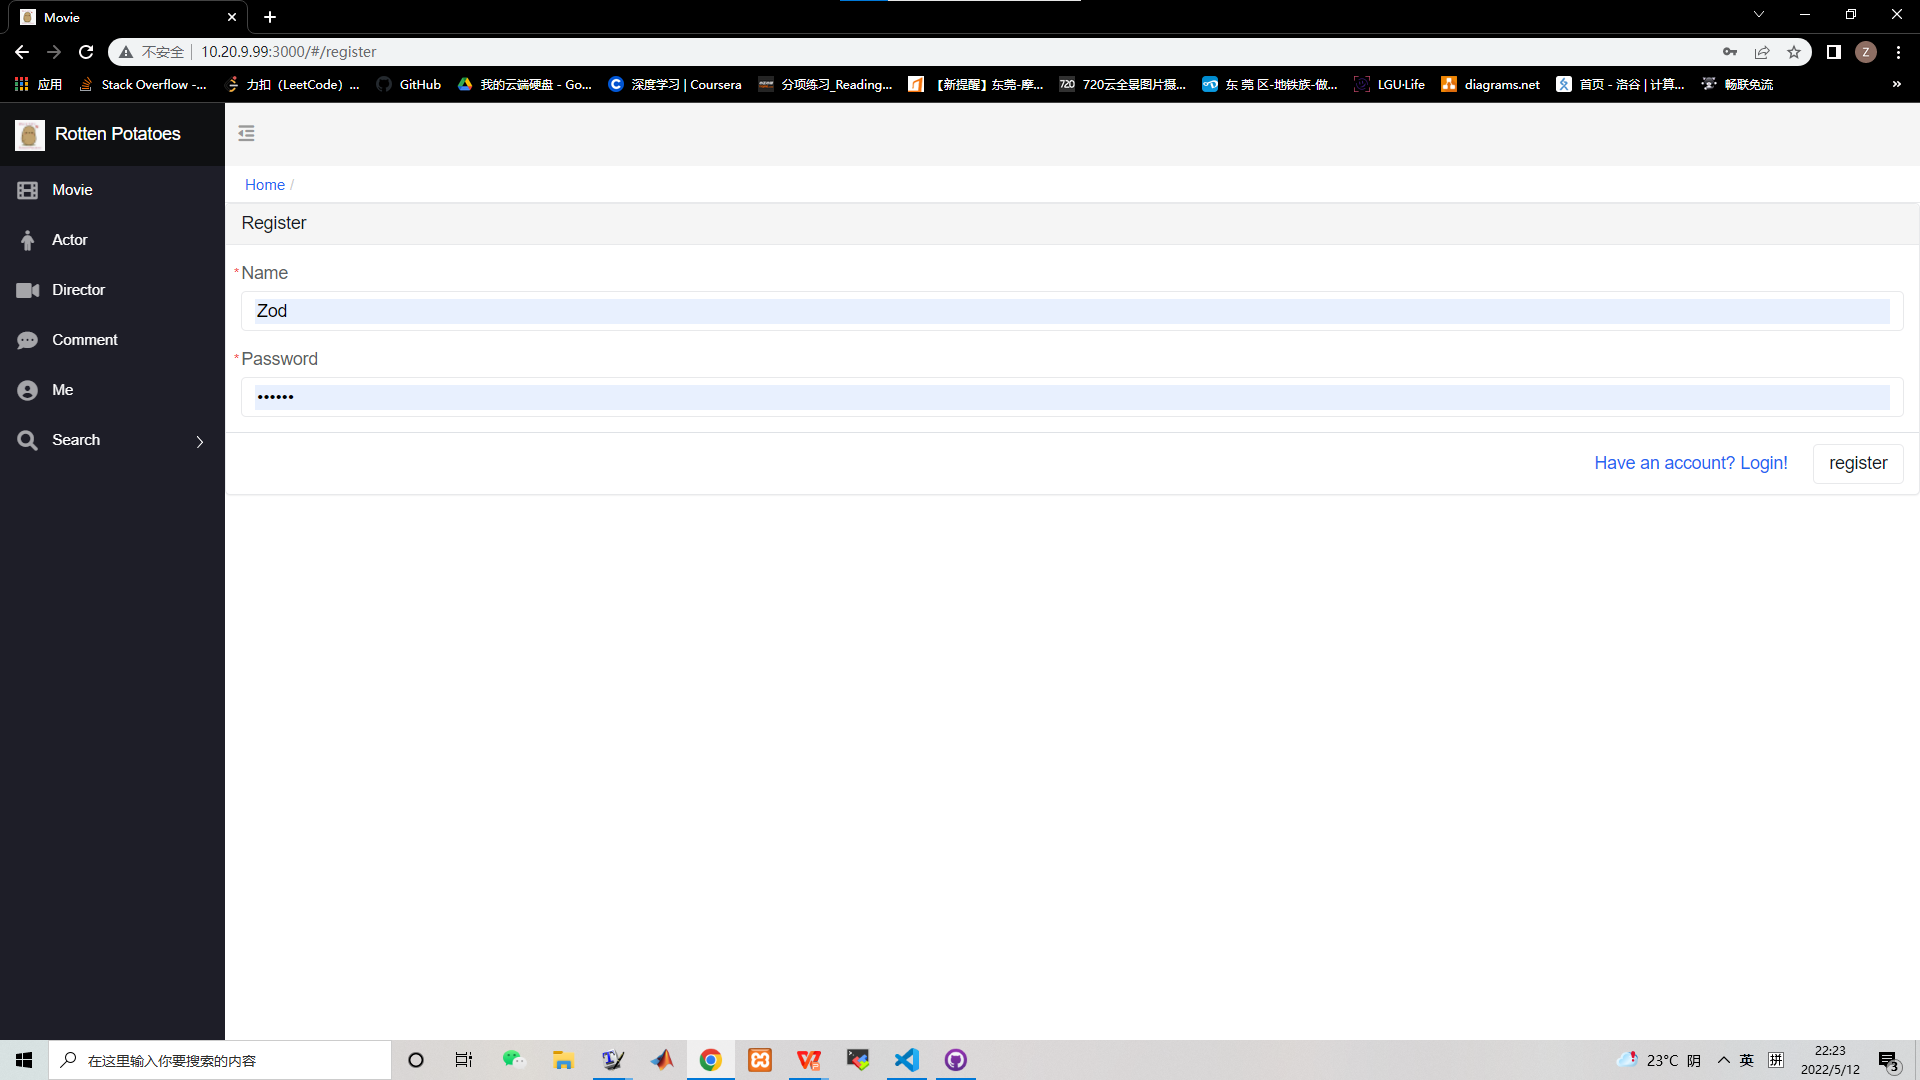
\includegraphics[width=1\textwidth]{reg.png}
    \caption{Register page}
    \end{figure}
    
    \begin{figure}[htbp]
    \centering
    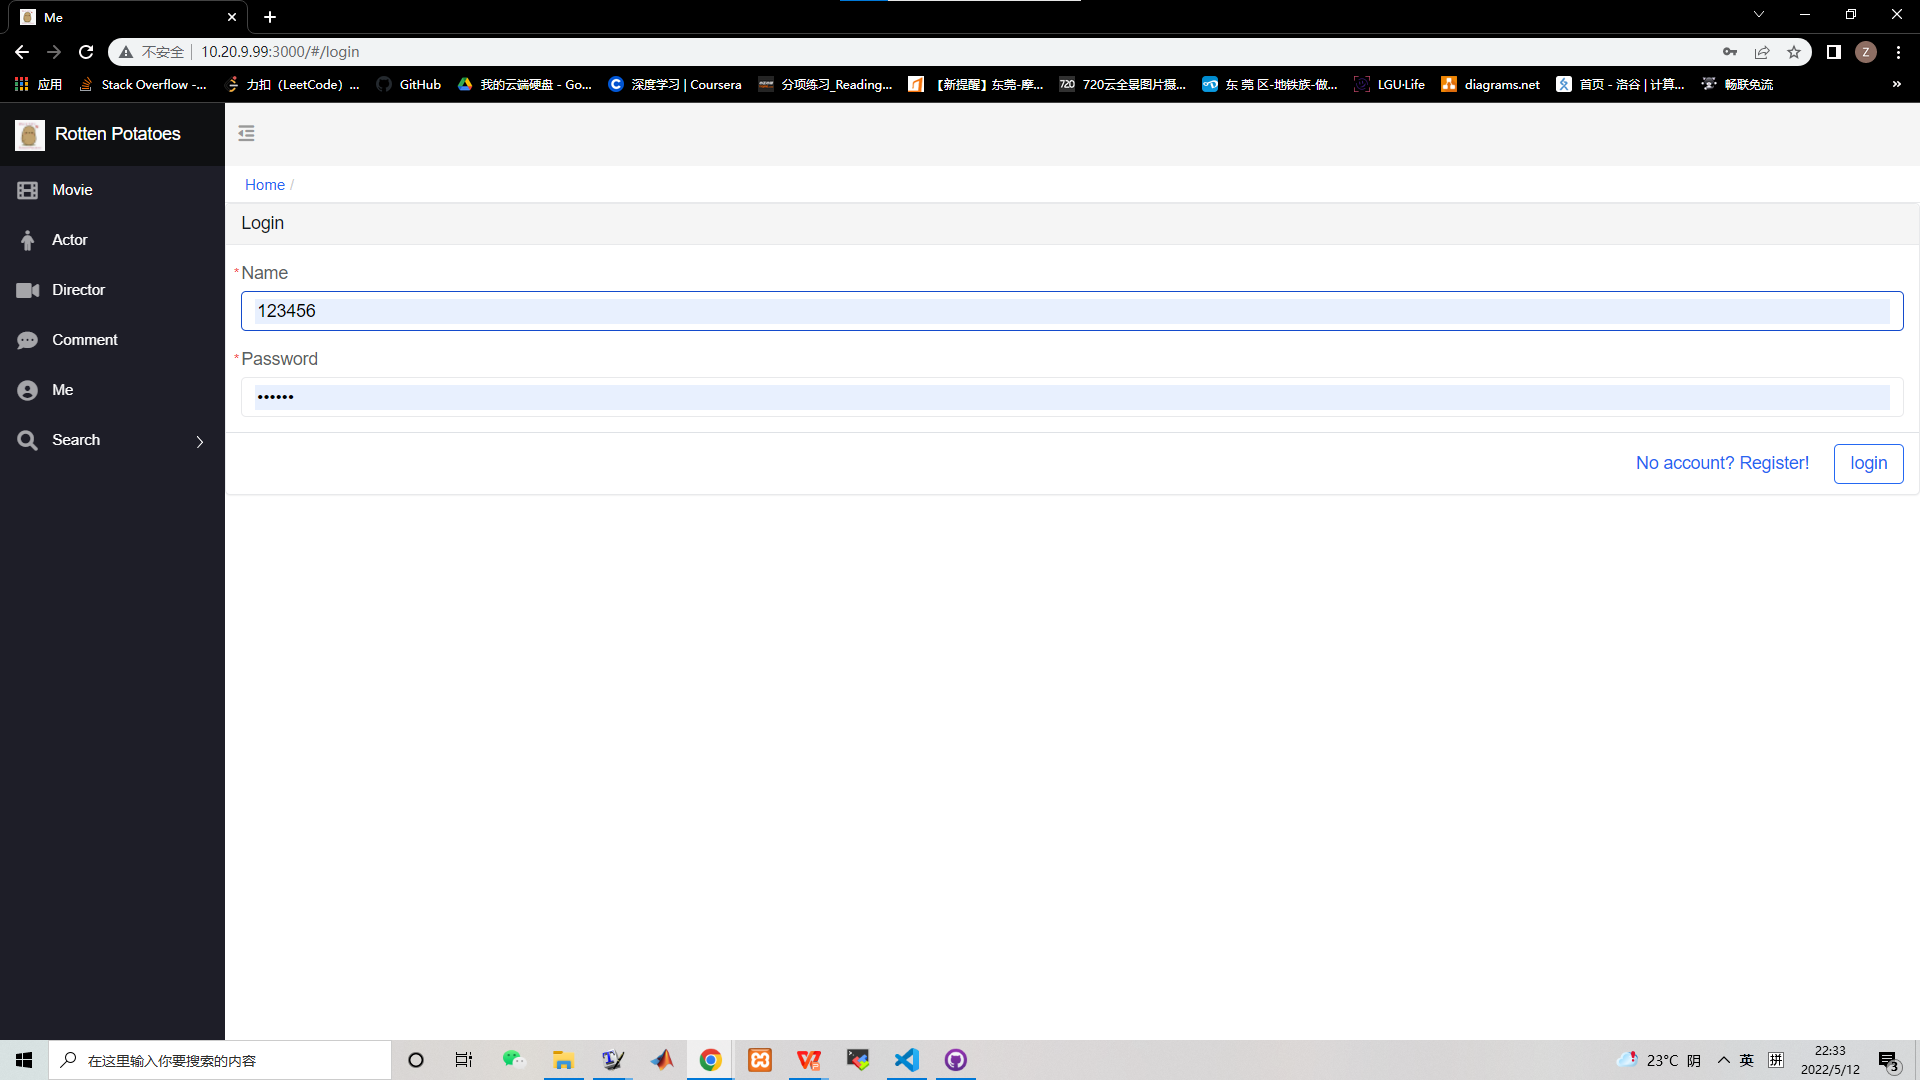
\includegraphics[width=1\textwidth]{res_login.png}
    \caption{Login page}
    \end{figure}
    
    \begin{figure}[htbp]
    \centering
    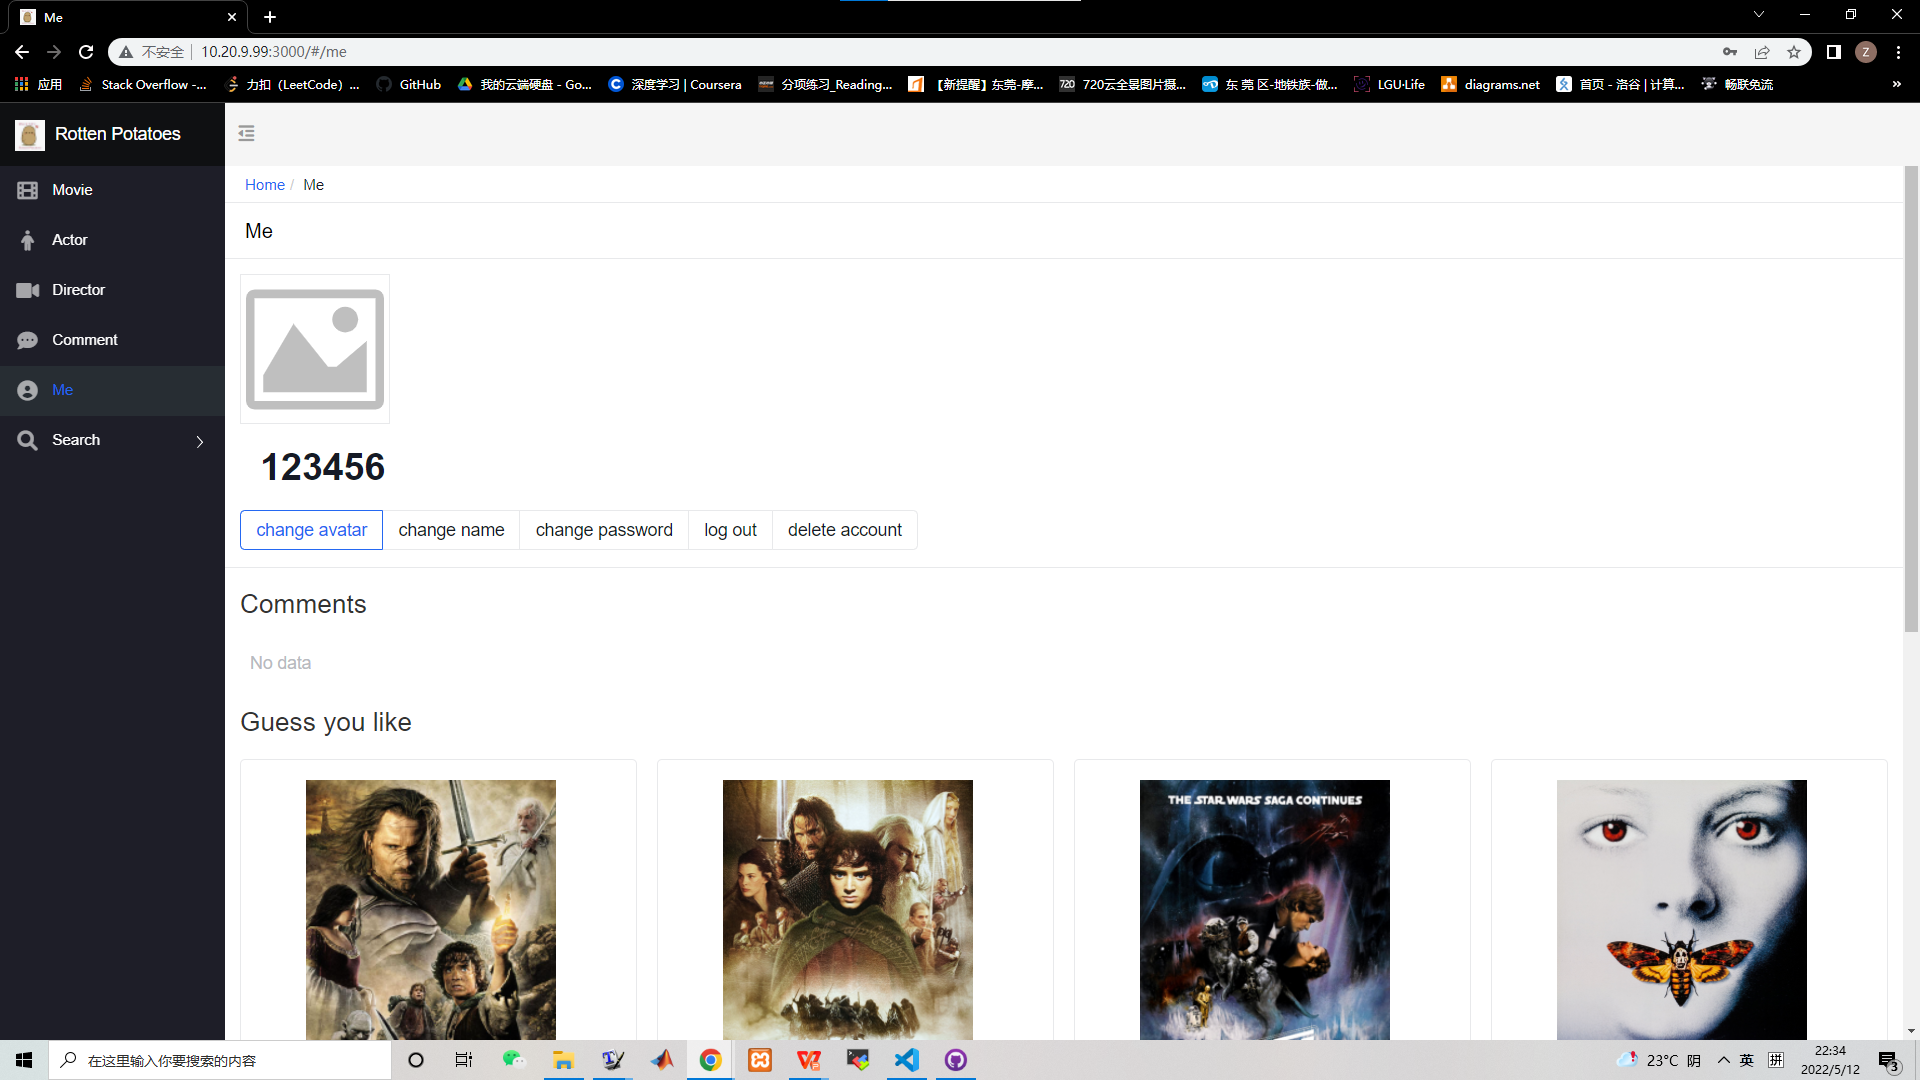
\includegraphics[width=1\textwidth]{res_ps.png}
    \caption{Personal center}
    \end{figure}
    
    \begin{figure}[htbp]
    \centering
    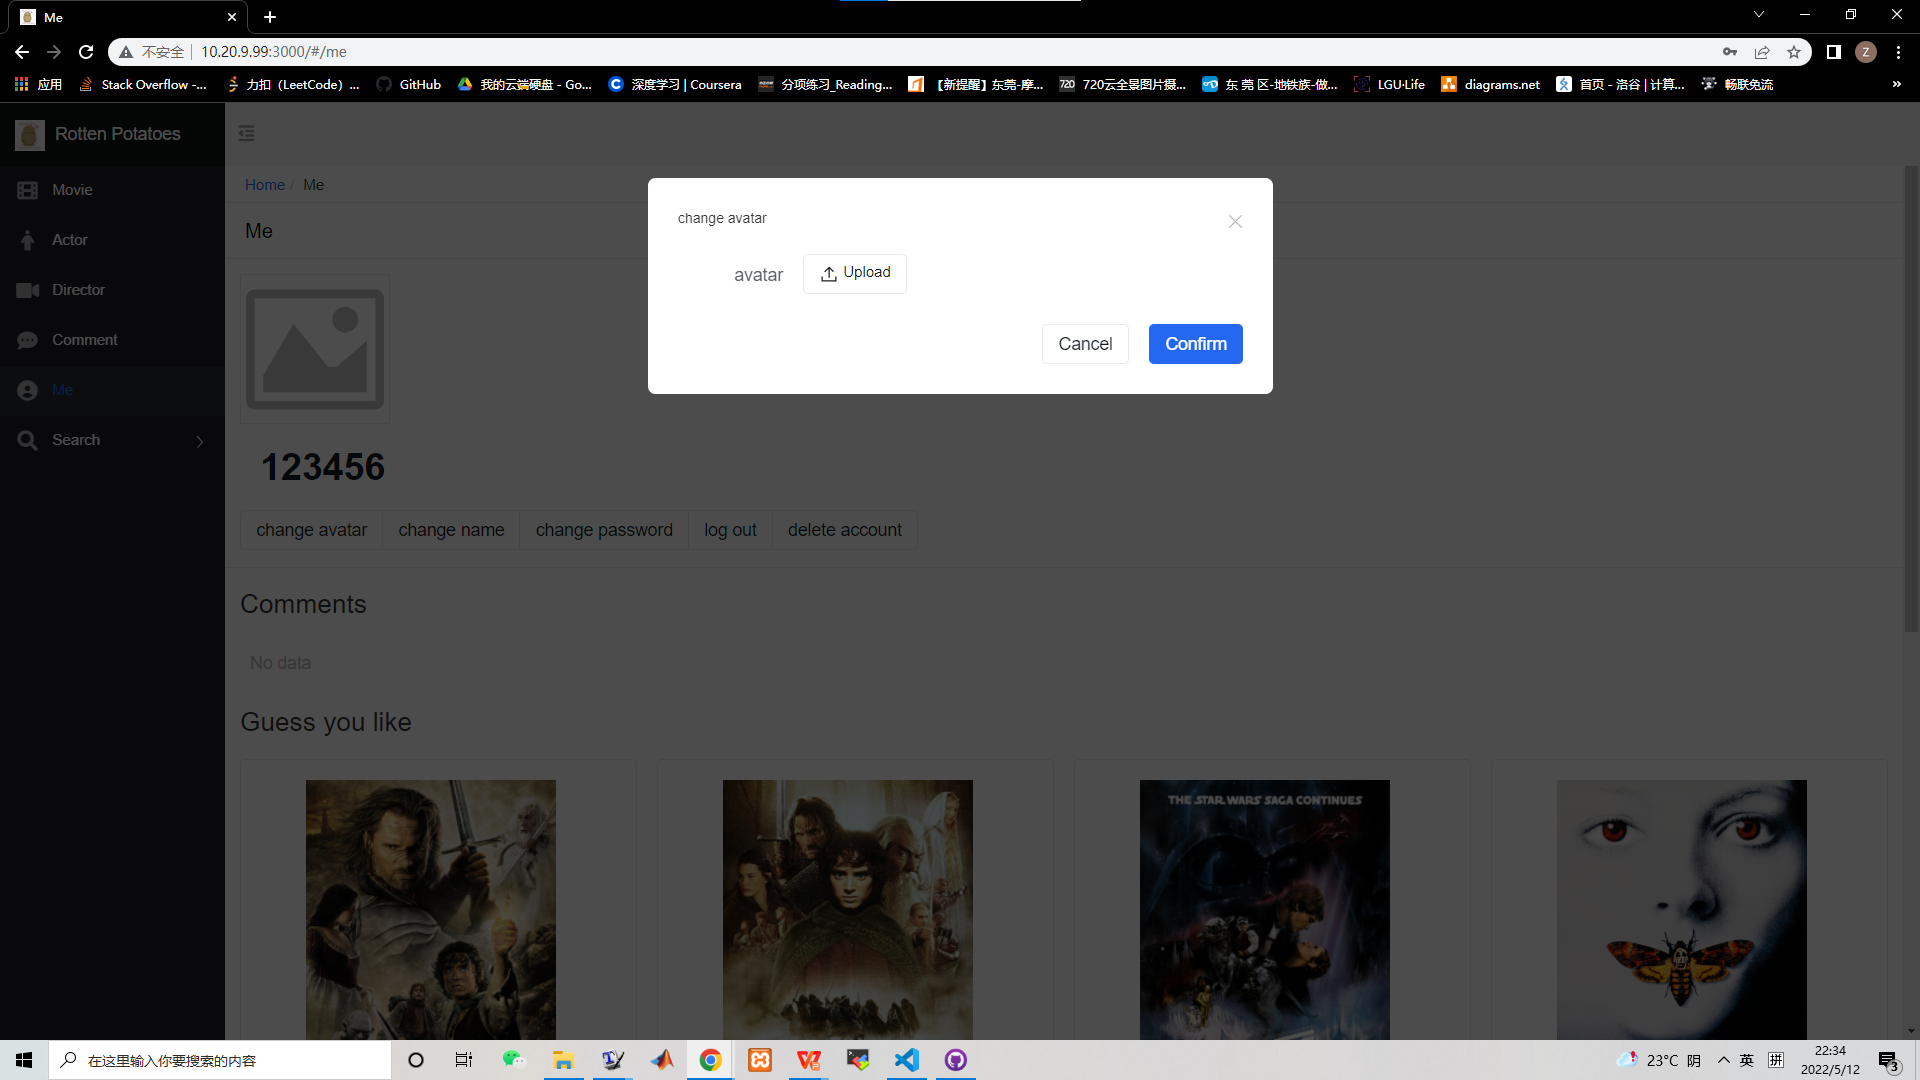
\includegraphics[width=0.9\textwidth]{res_avatar1.png}
    \caption{Before chaning avatar}
    \end{figure}
    
    \begin{figure}[htbp]
    \centering
    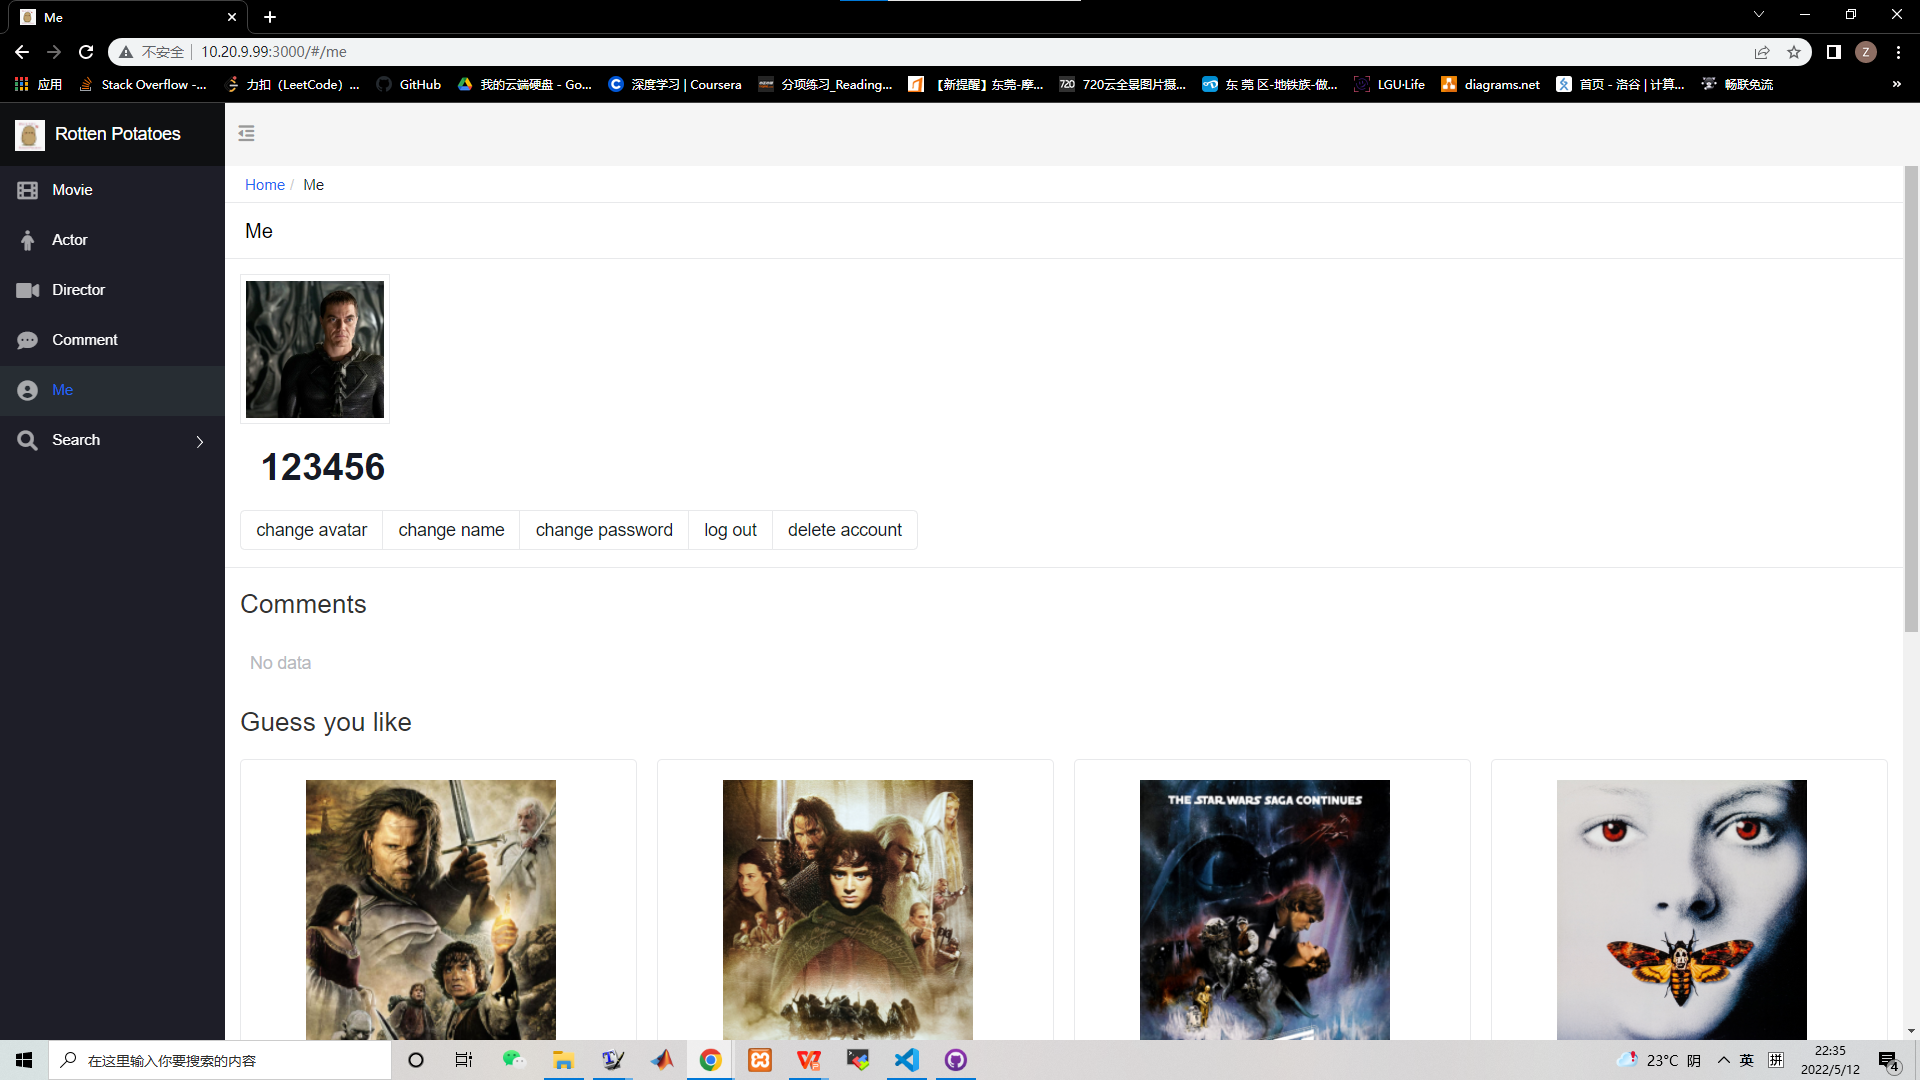
\includegraphics[width=1\textwidth]{res_avatar2.png}
    \caption{After chaning avatar}
    \end{figure}
    
    \begin{figure}[htbp]
    \centering
    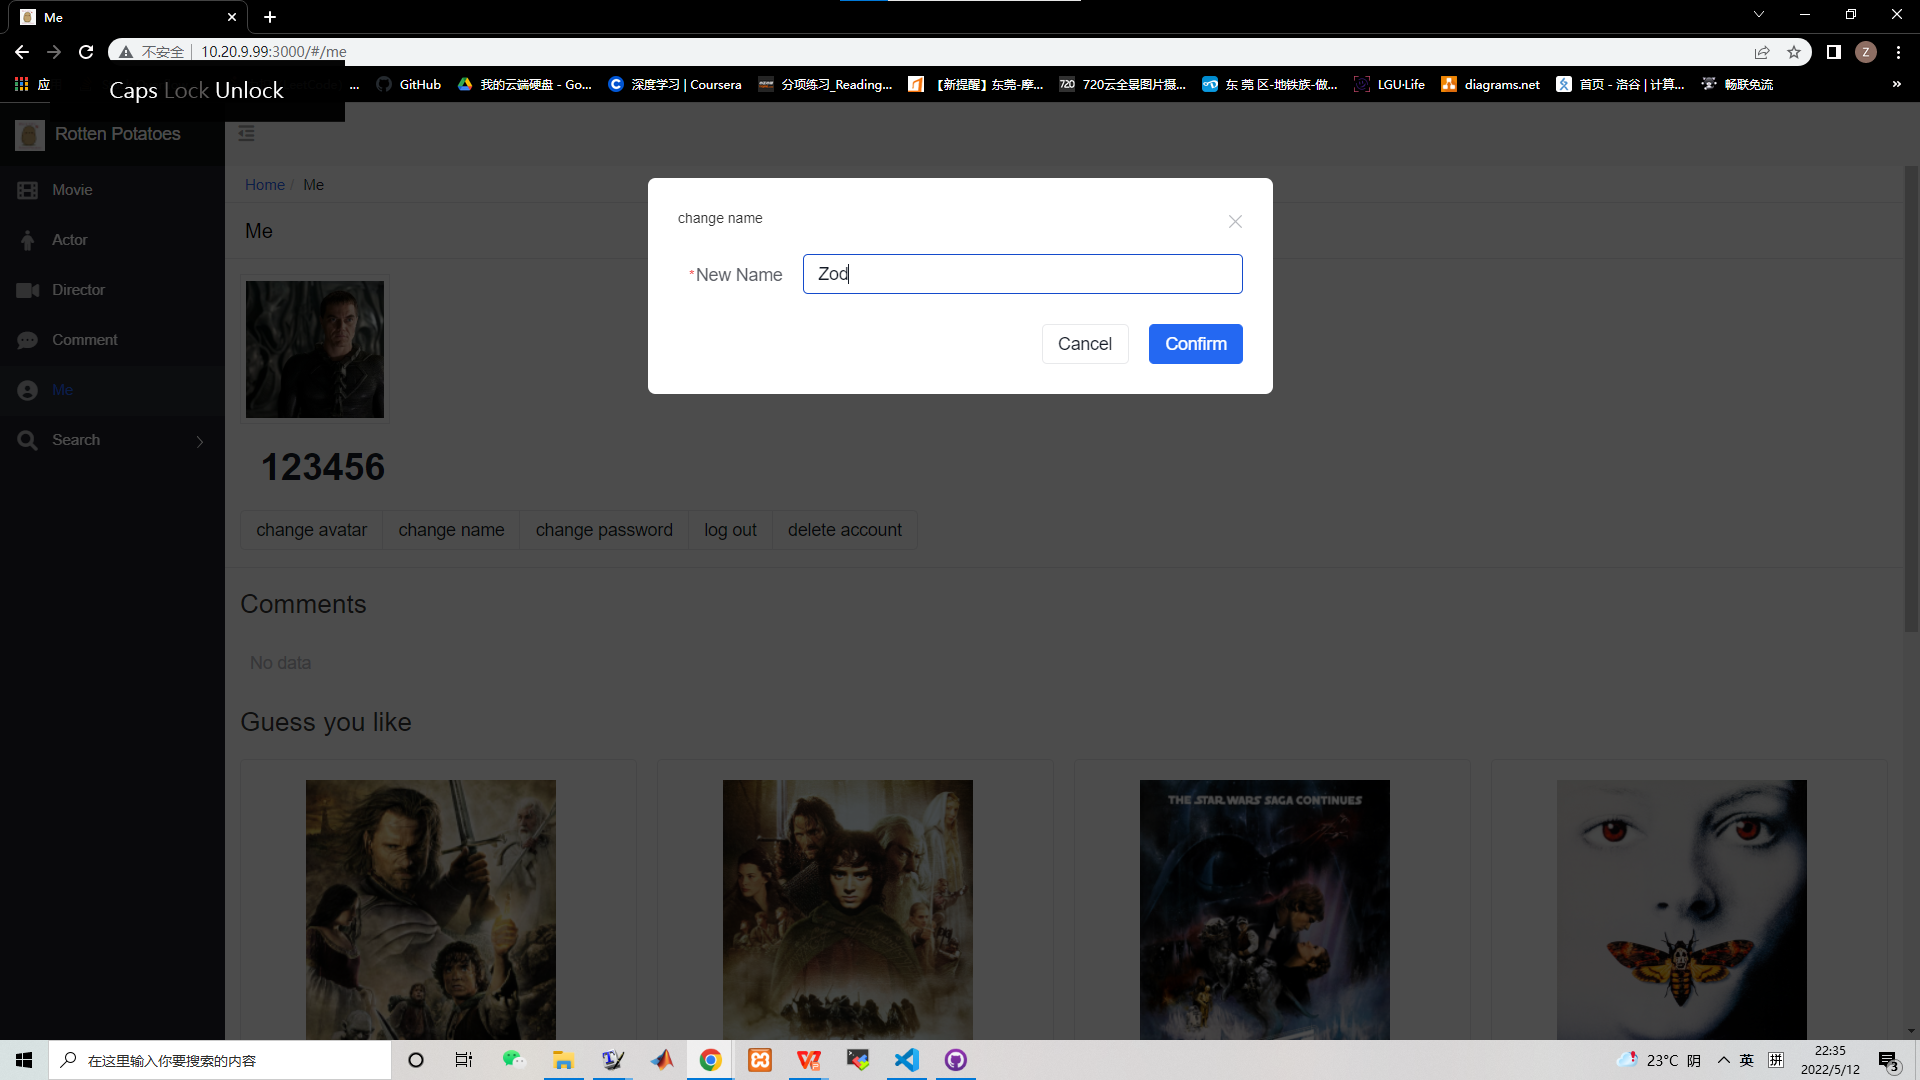
\includegraphics[width=1\textwidth]{res_name1.png}
    \caption{Before chaning name}
    \end{figure}
    
    \begin{figure}[htbp]
    \centering
    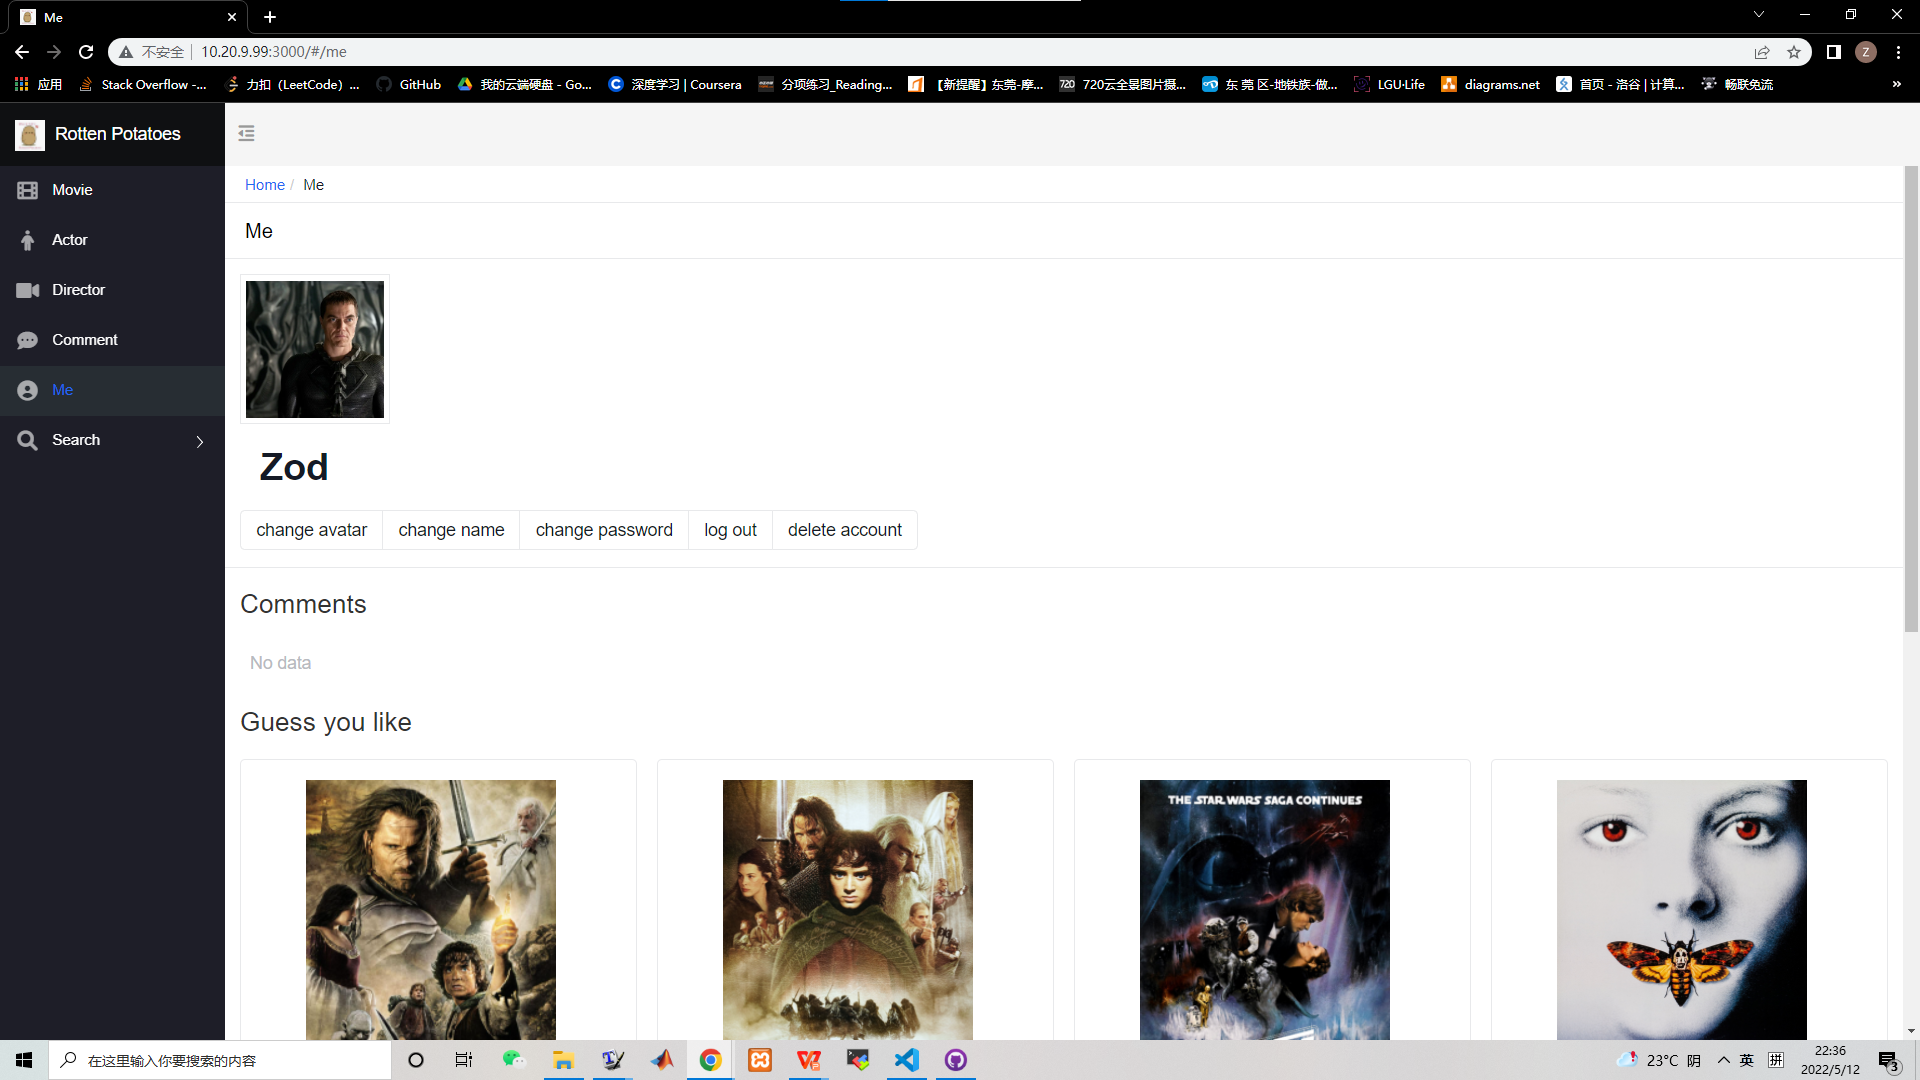
\includegraphics[width=1\textwidth]{res_name2.png}
    \caption{After chaning name}
    \end{figure}
    
    \begin{figure}[htbp]
    \centering
    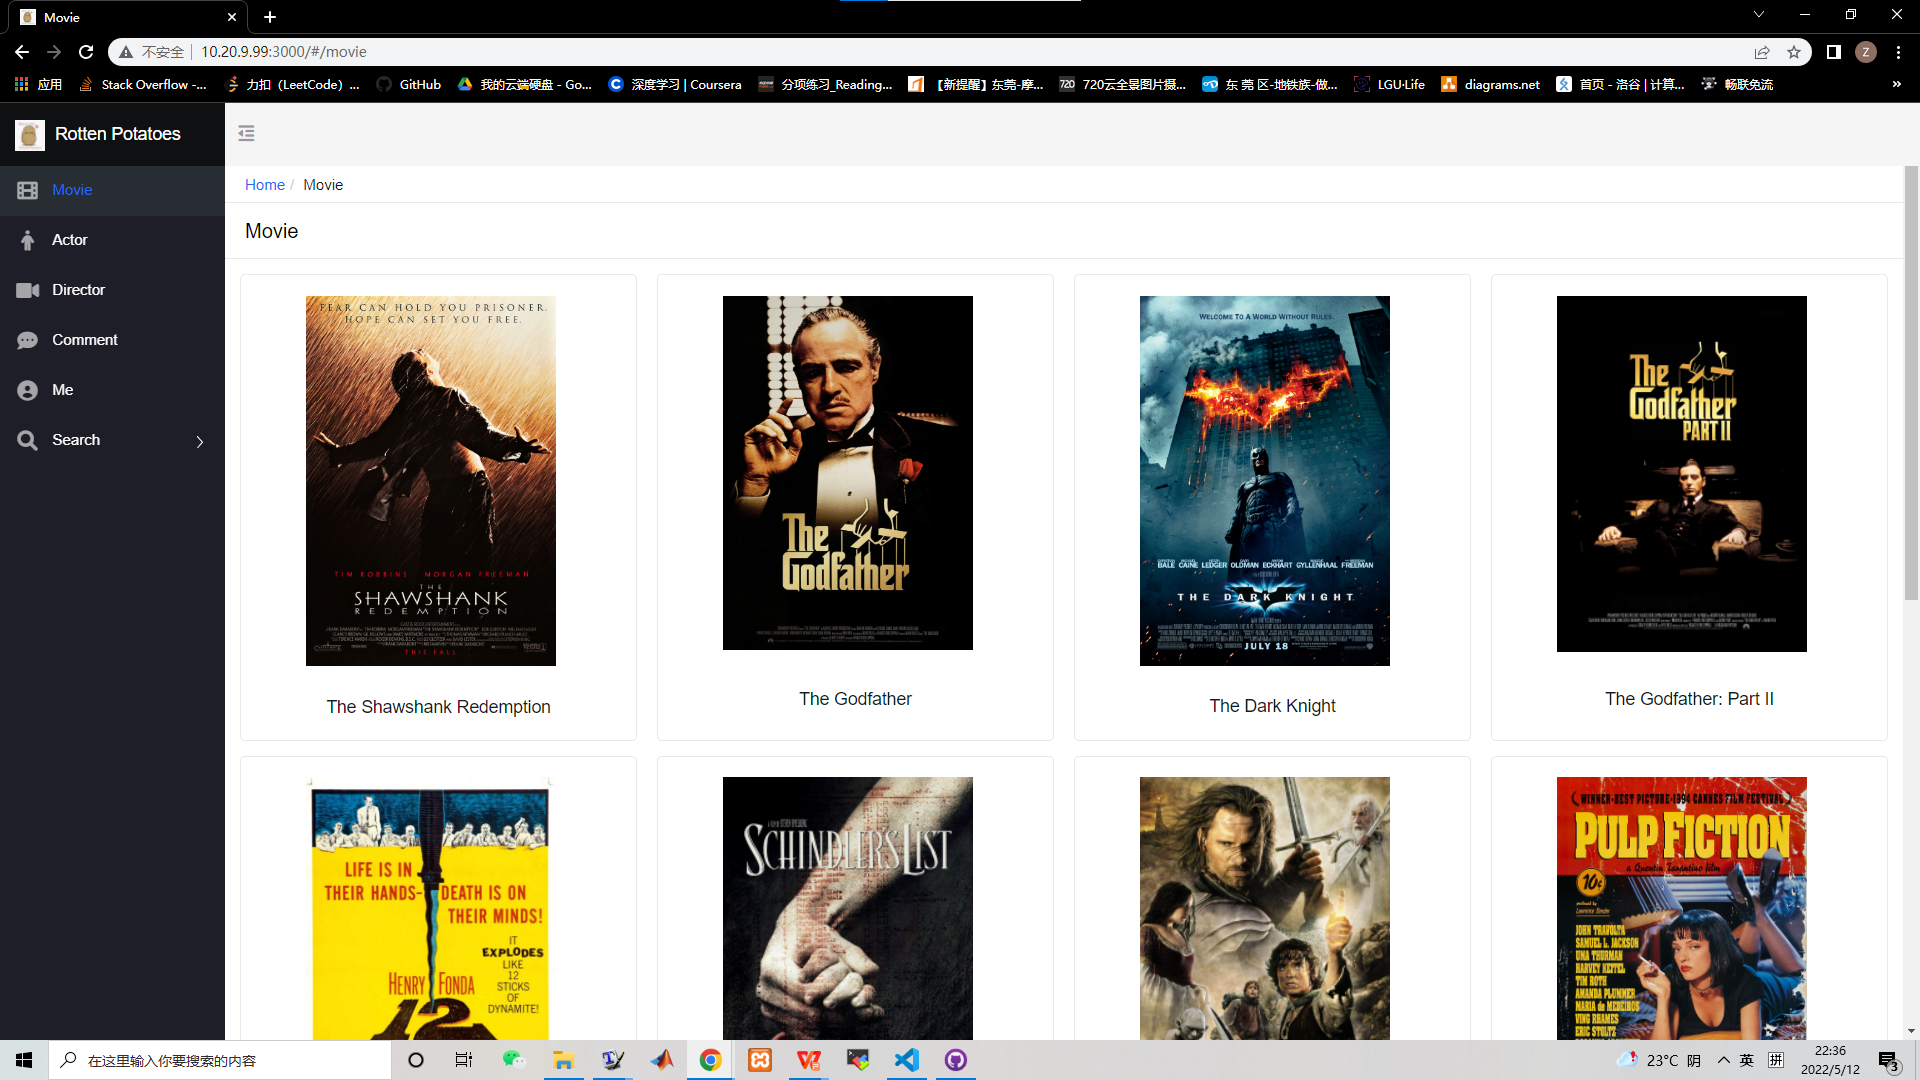
\includegraphics[width=1\textwidth]{res_movie1.png}
    \caption{Movie list page}
    \end{figure}
    
    \begin{figure}[htbp]
    \centering
    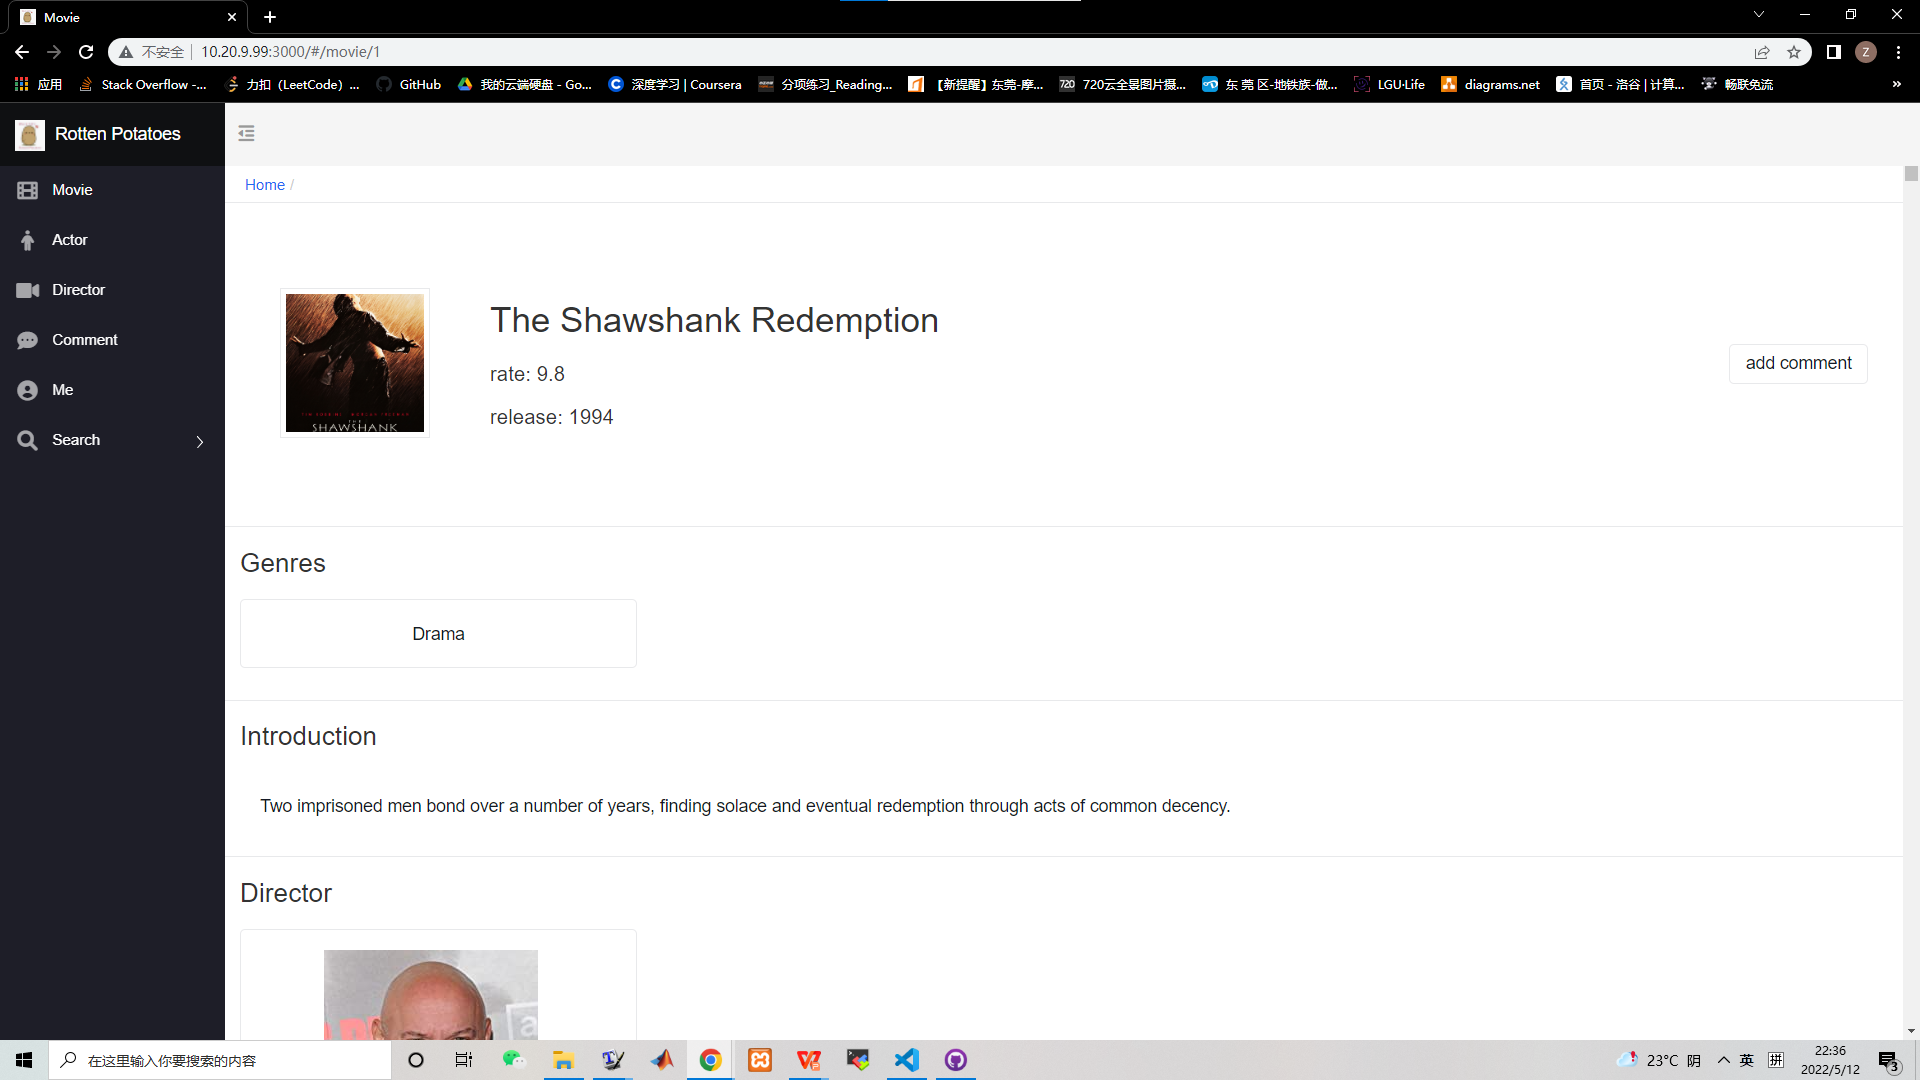
\includegraphics[width=1\textwidth]{res_movie2.png}
    \caption{Movie detail page}
    \end{figure}
    
    \begin{figure}[htbp]
    \centering
    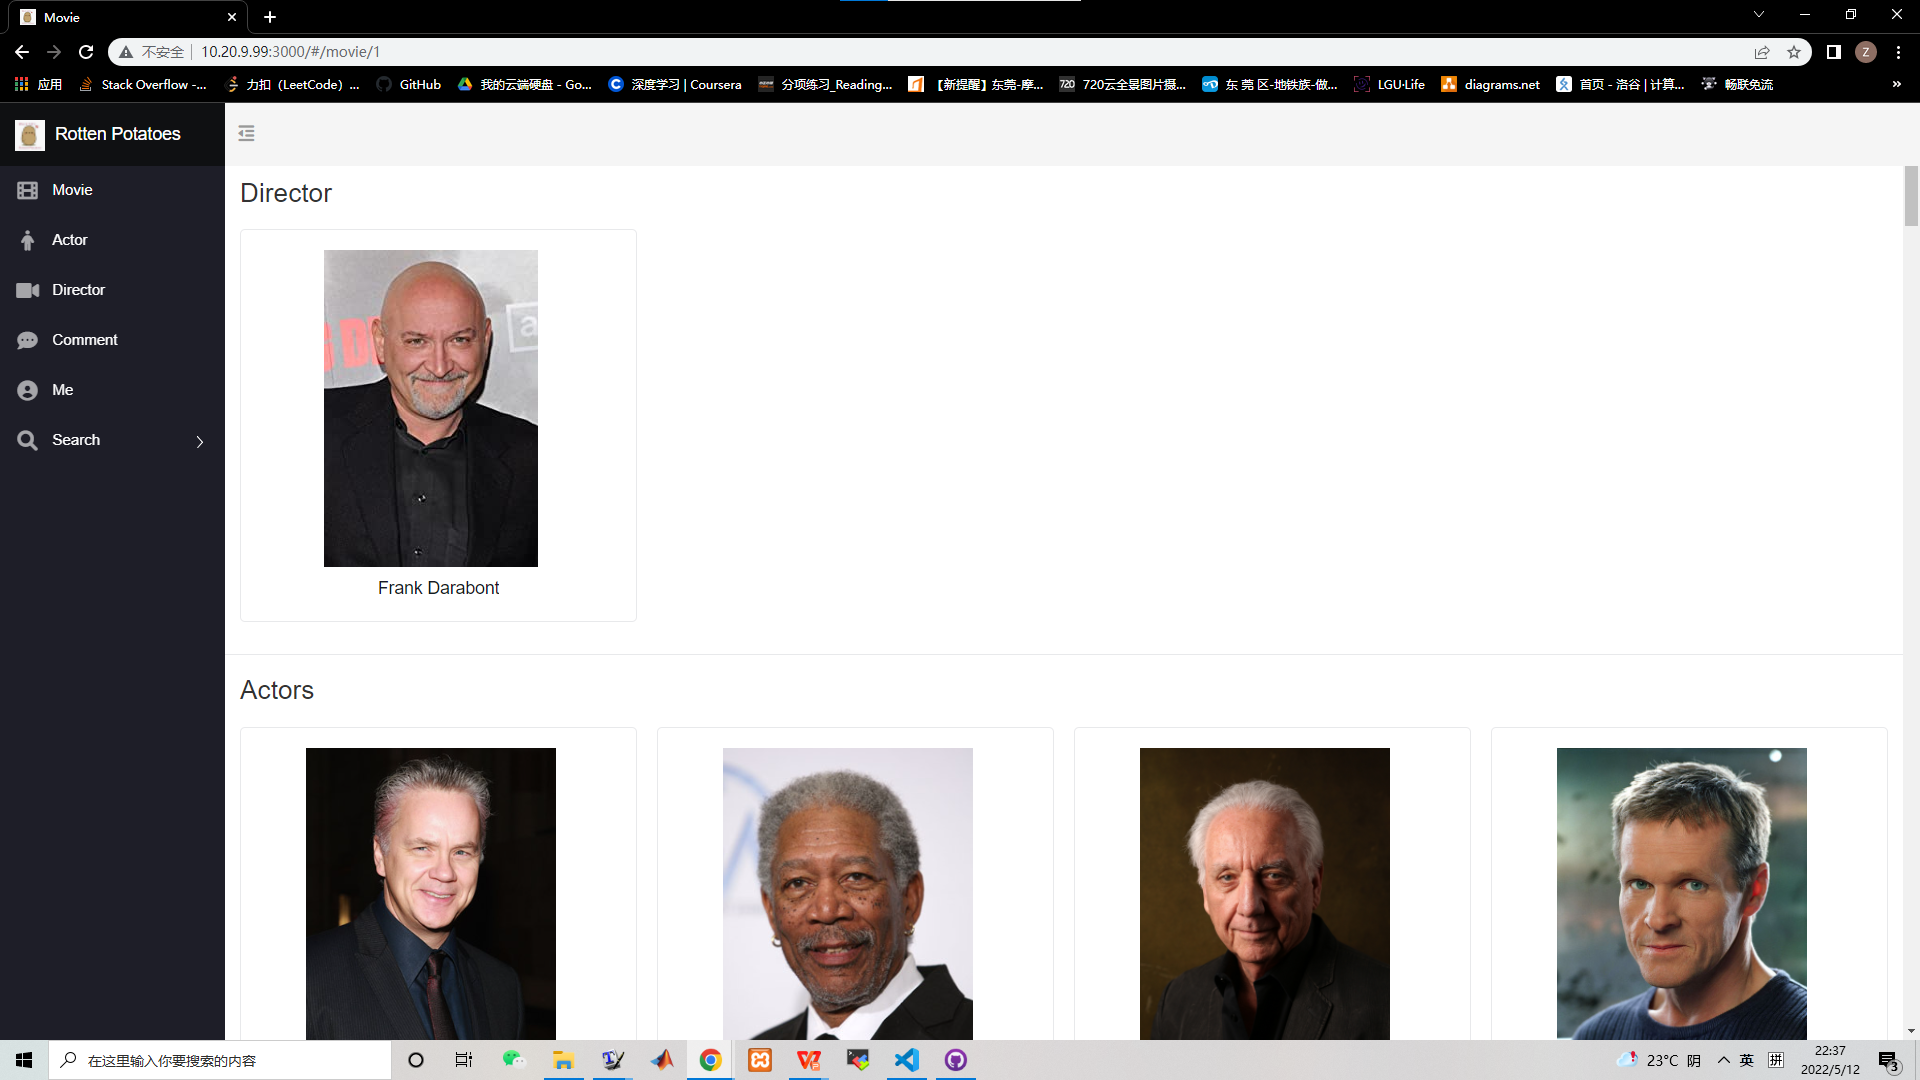
\includegraphics[width=1\textwidth]{res_movie3.png}
    \caption{Movie detail page}
    \end{figure}
    
    \begin{figure}[htbp]
    \centering
    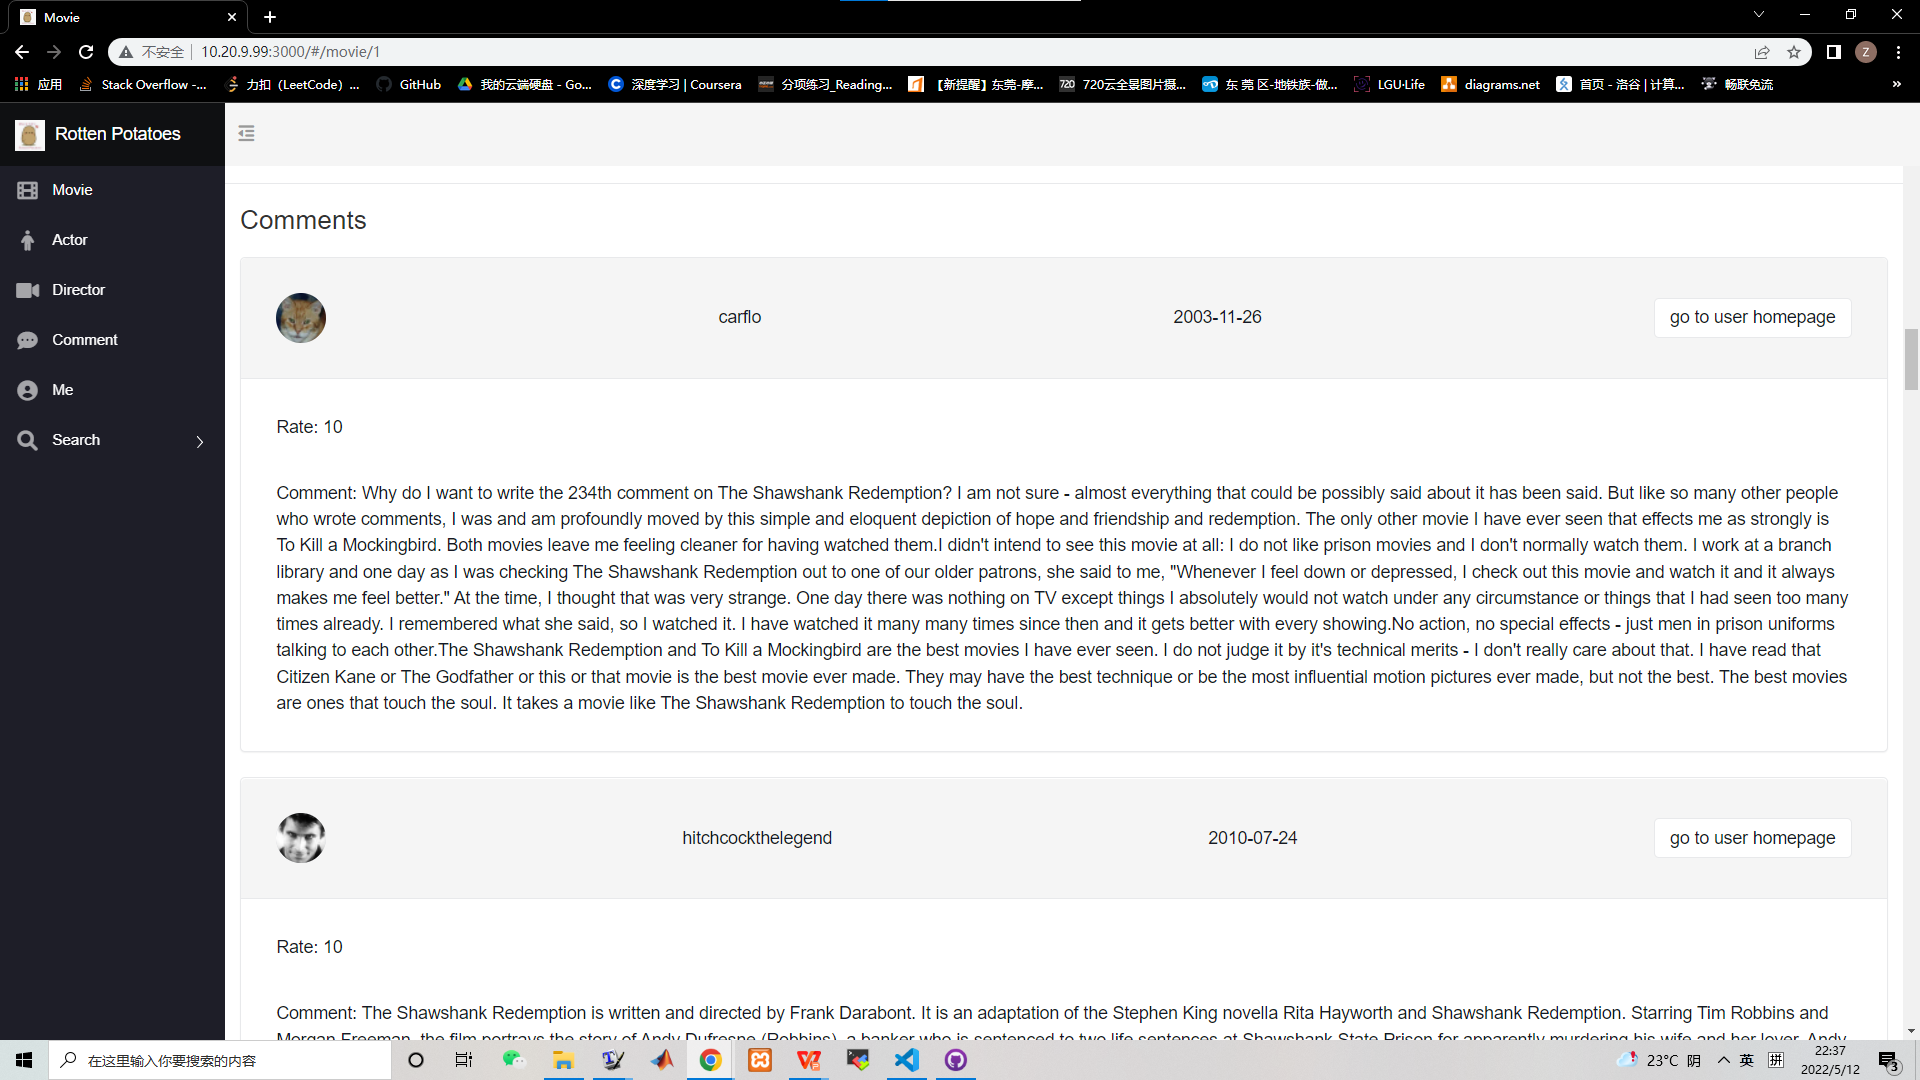
\includegraphics[width=1\textwidth]{res_movie4.png}
    \caption{Movie detail page}
    \end{figure}
    
    \begin{figure}[htbp]
    \centering
    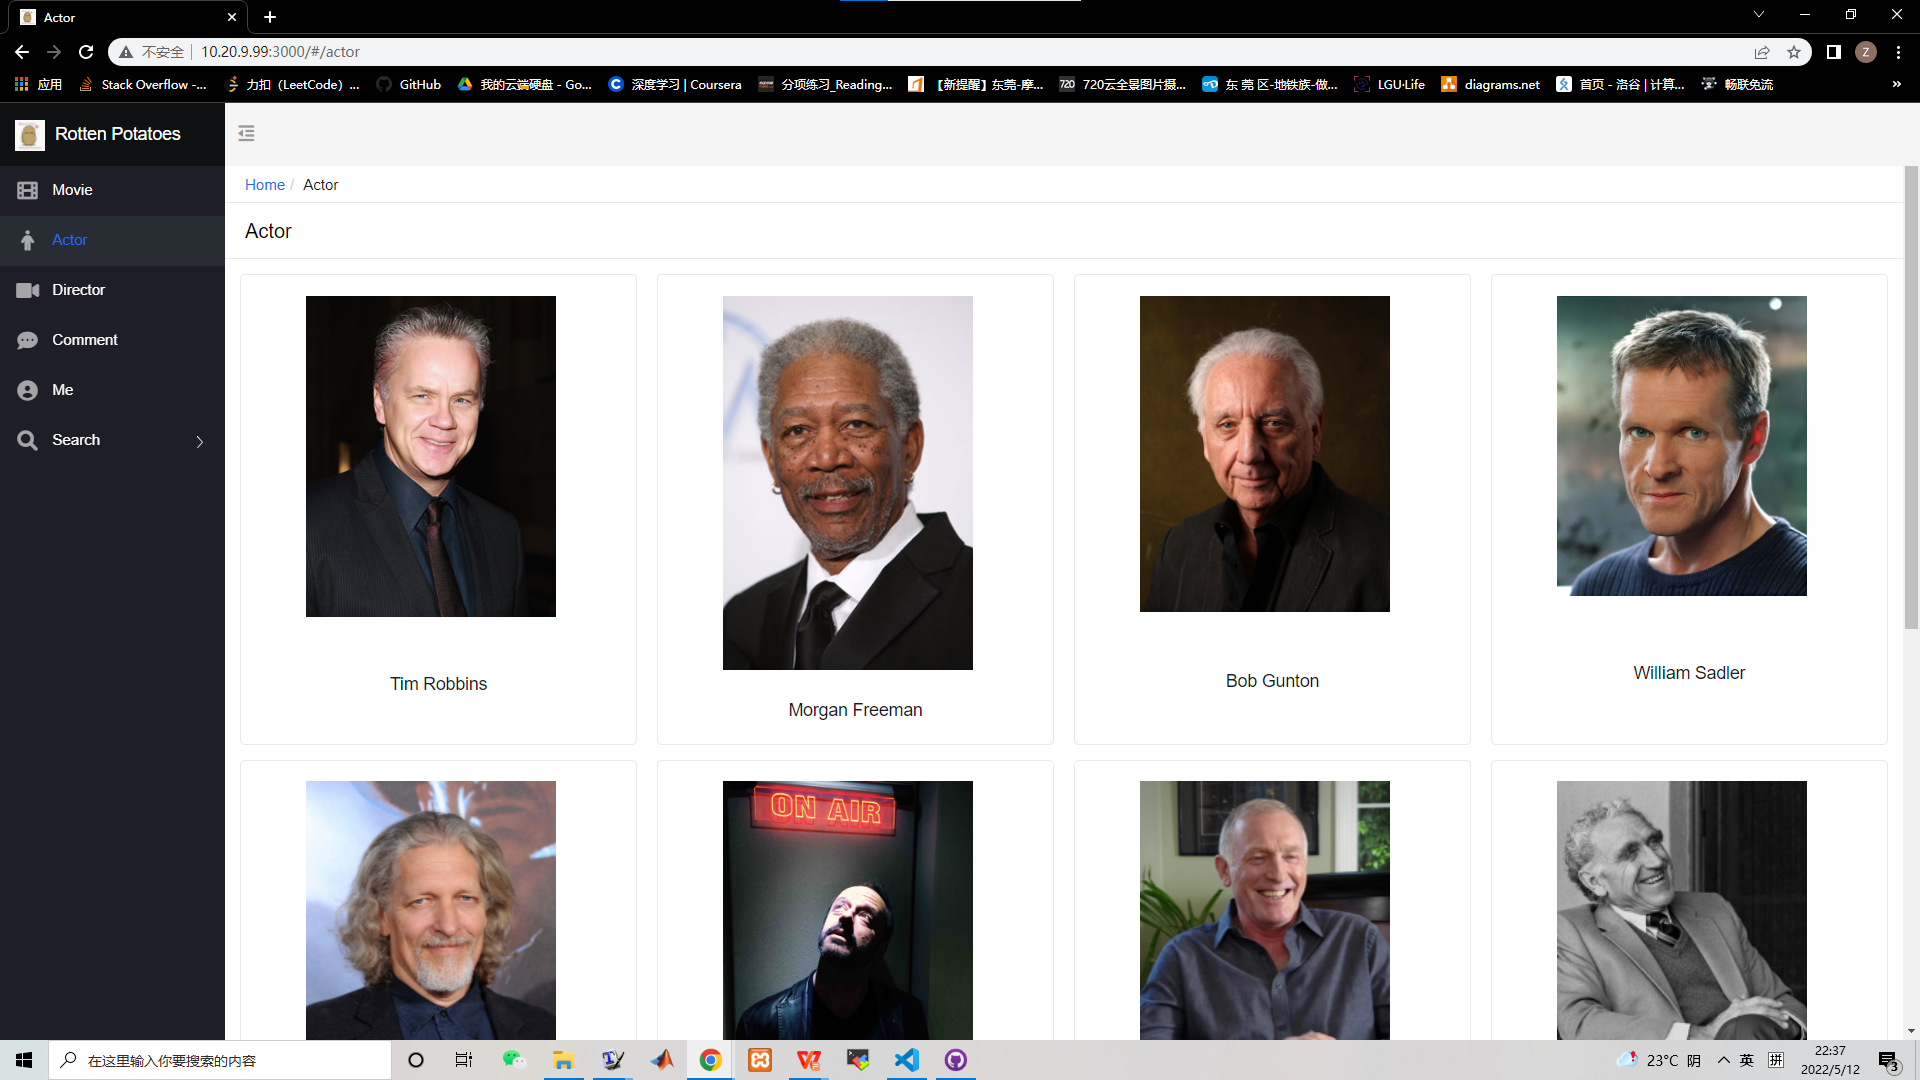
\includegraphics[width=1\textwidth]{res_actor1.png}
    \caption{Actor list page}
    \end{figure}
    
    \begin{figure}[htbp]
    \centering
    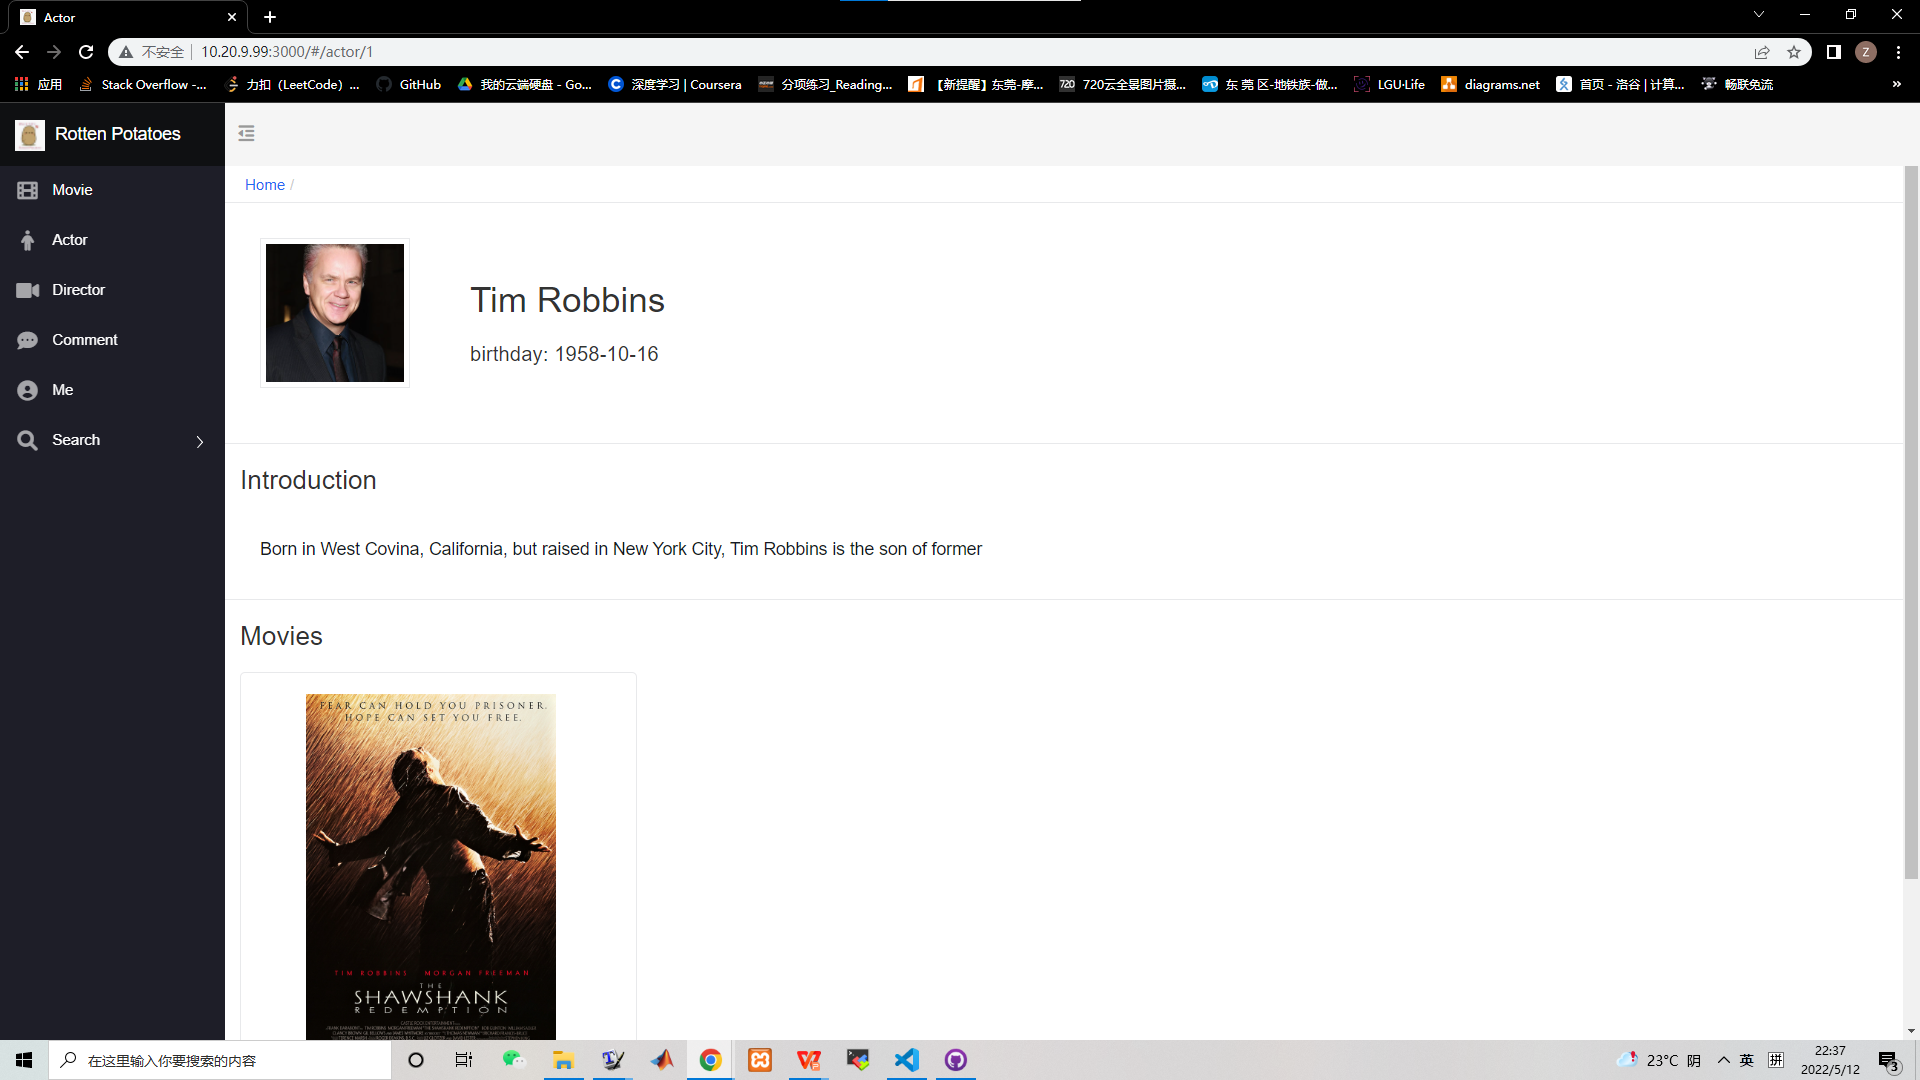
\includegraphics[width=1\textwidth]{res_actor2.png}
    \caption{Actor detail page}
    \end{figure}
    
    \begin{figure}[htbp]
    \centering
    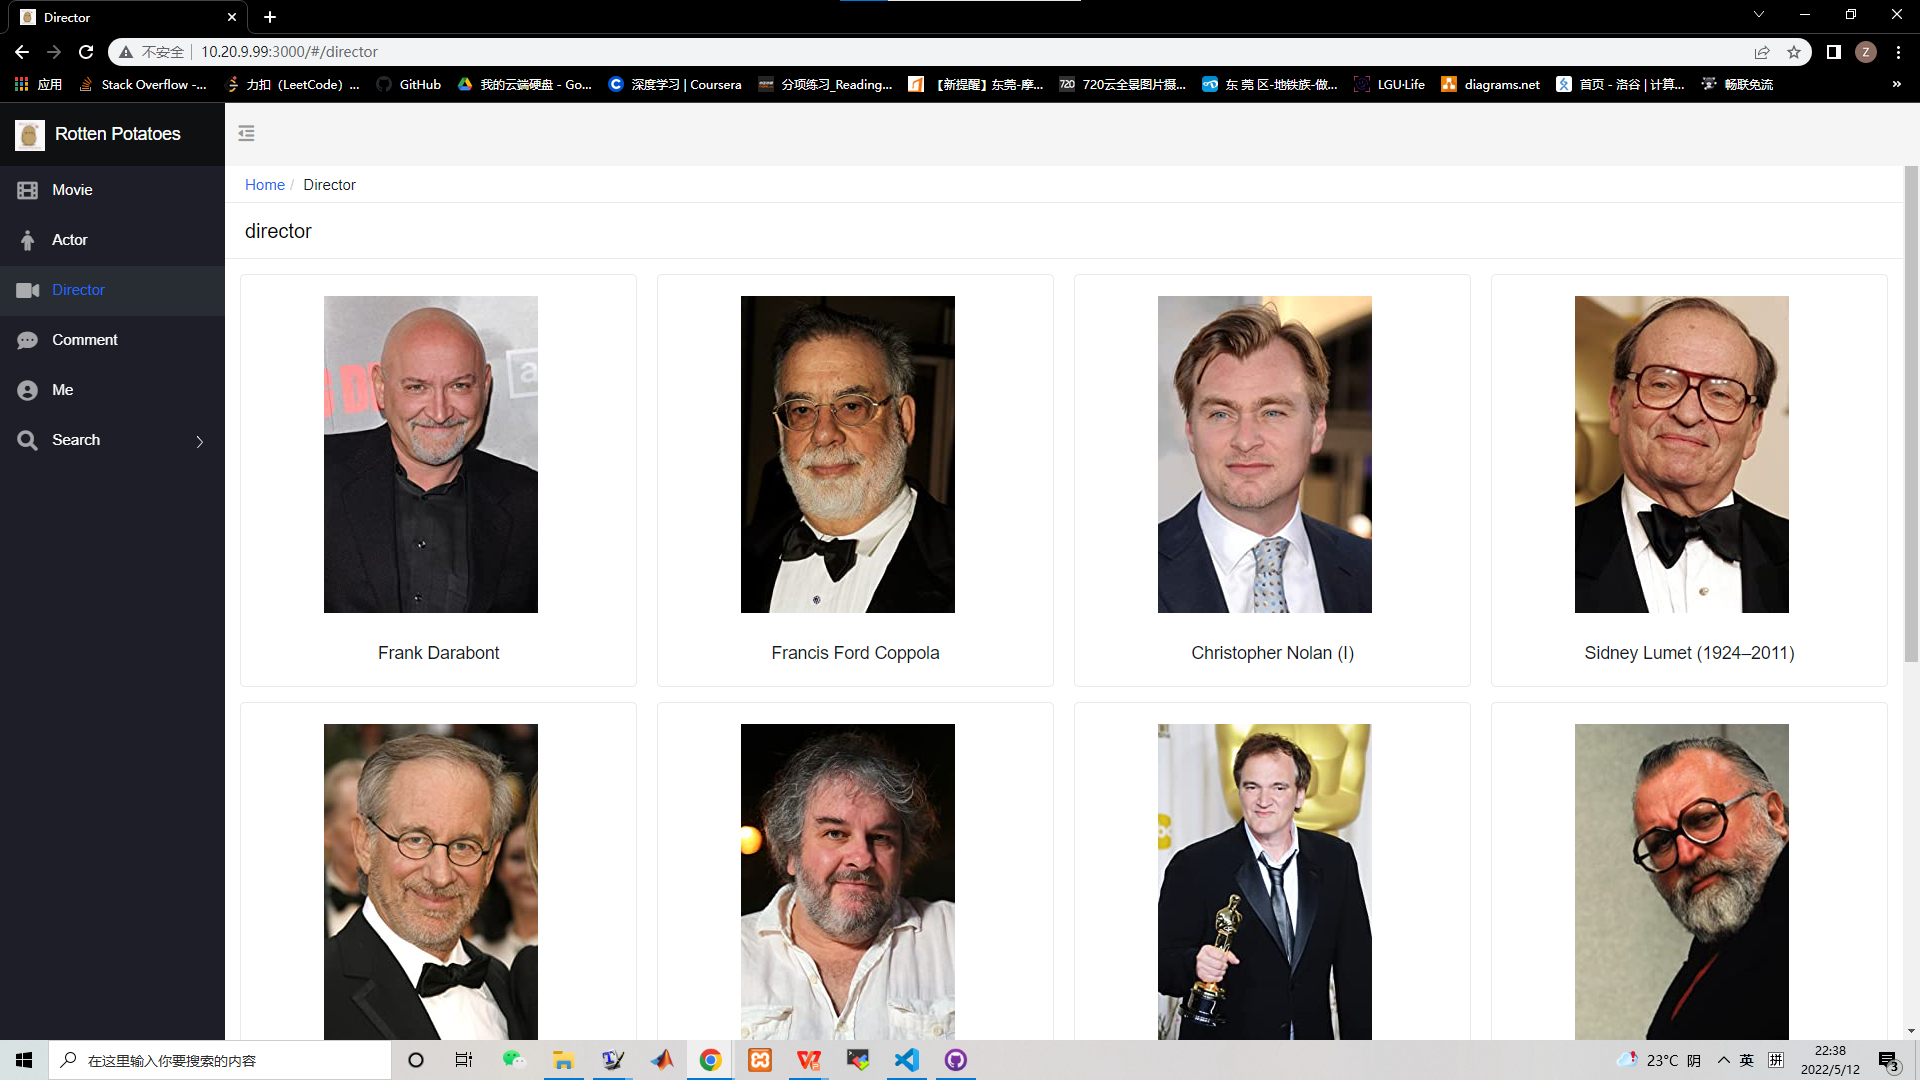
\includegraphics[width=1\textwidth]{res_dir1.png}
    \caption{Director list page}
    \end{figure}
    
    \begin{figure}[htbp]
    \centering
    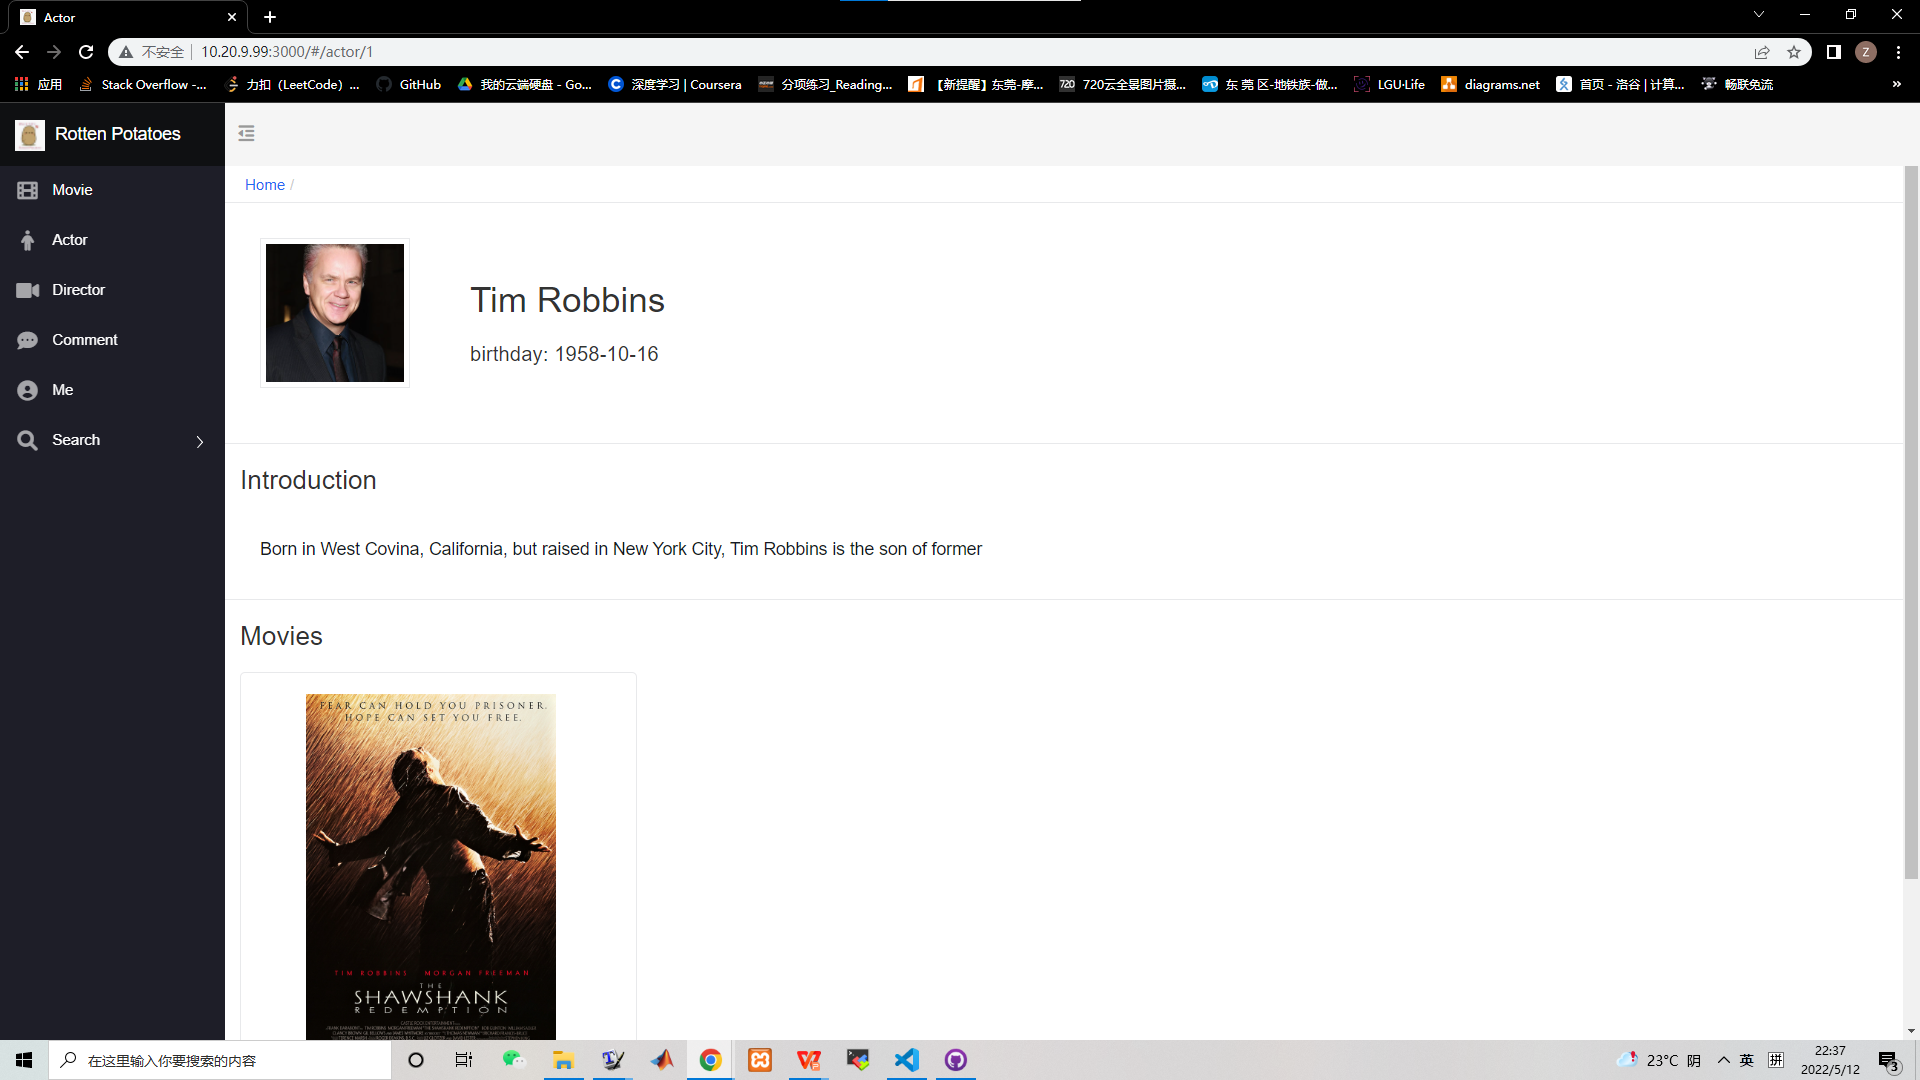
\includegraphics[width=1\textwidth]{res_actor2.png}
    \caption{Director detail page}
    \end{figure}
    
    \begin{figure}[htbp]
    \centering
    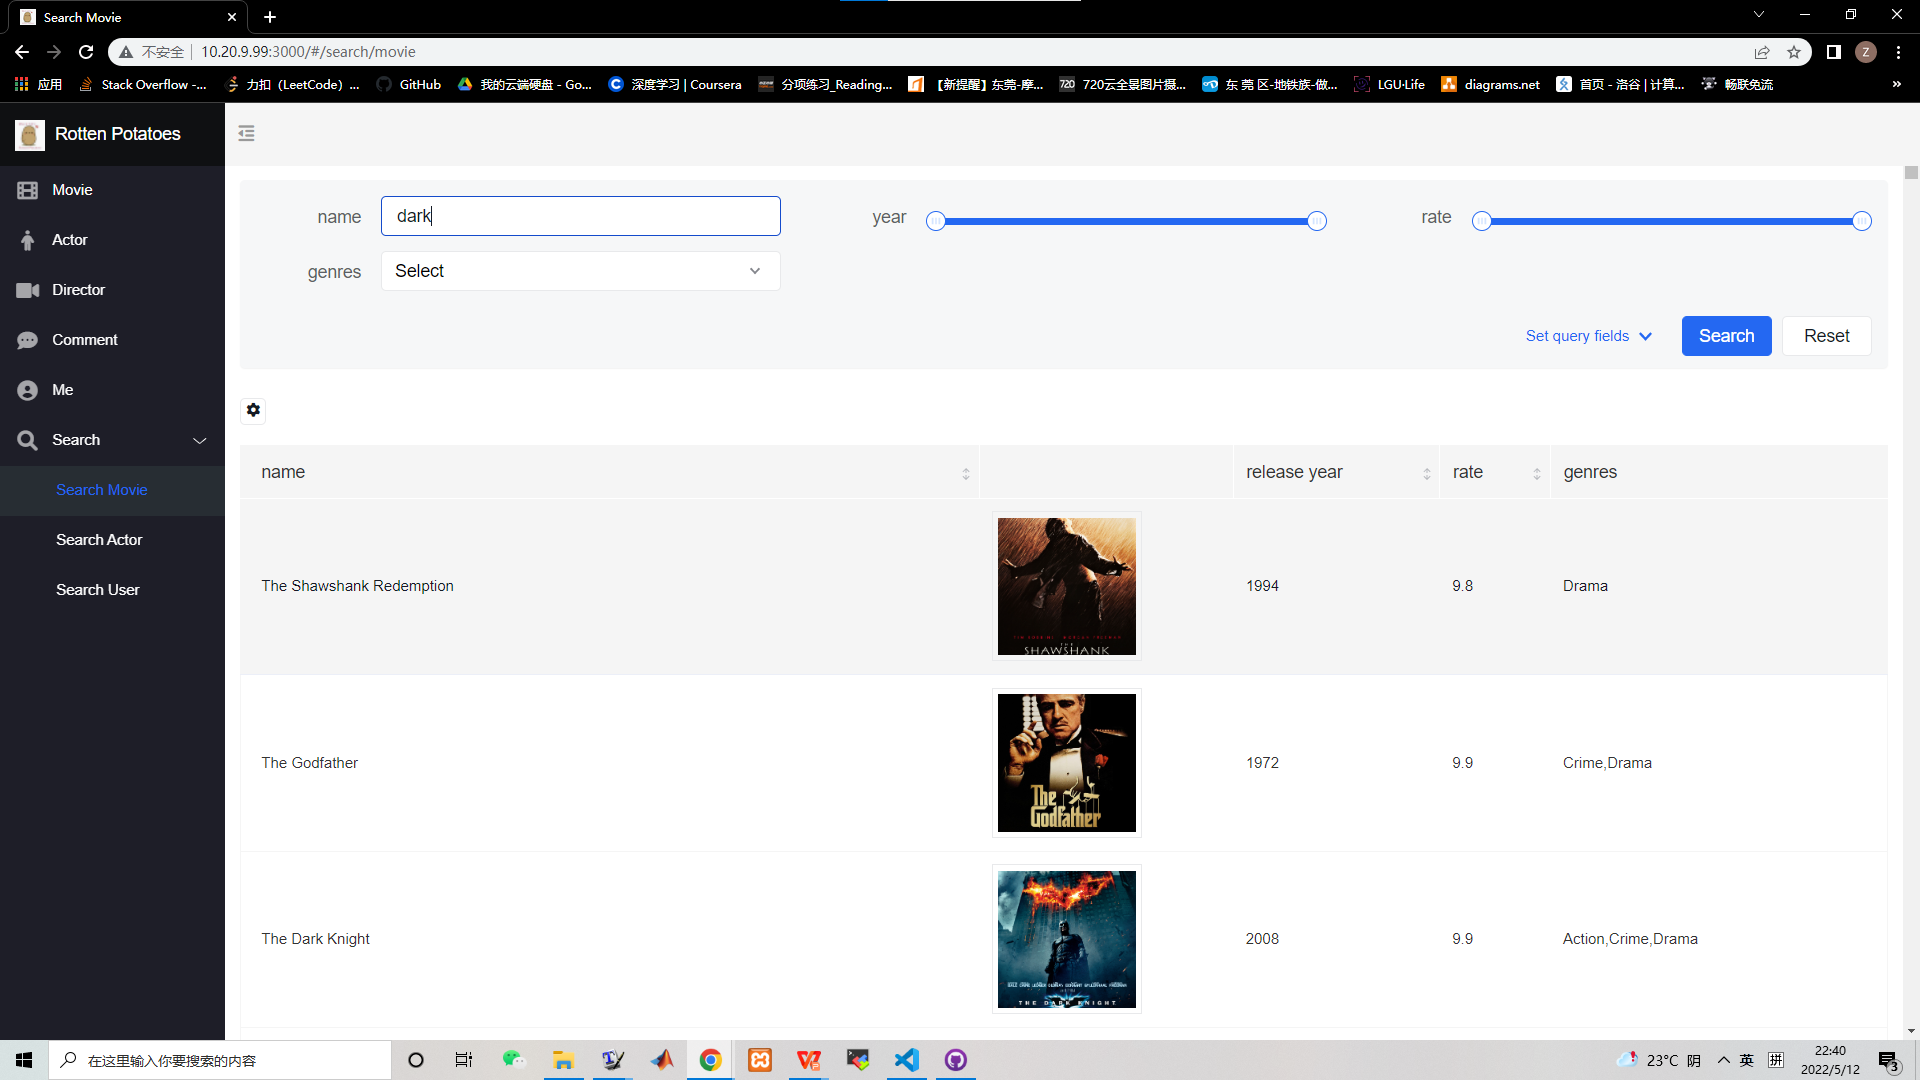
\includegraphics[width=1\textwidth]{res_search1.png}
    \caption{Movie search page}
    \end{figure}
    
    \begin{figure}[htbp]
    \centering
    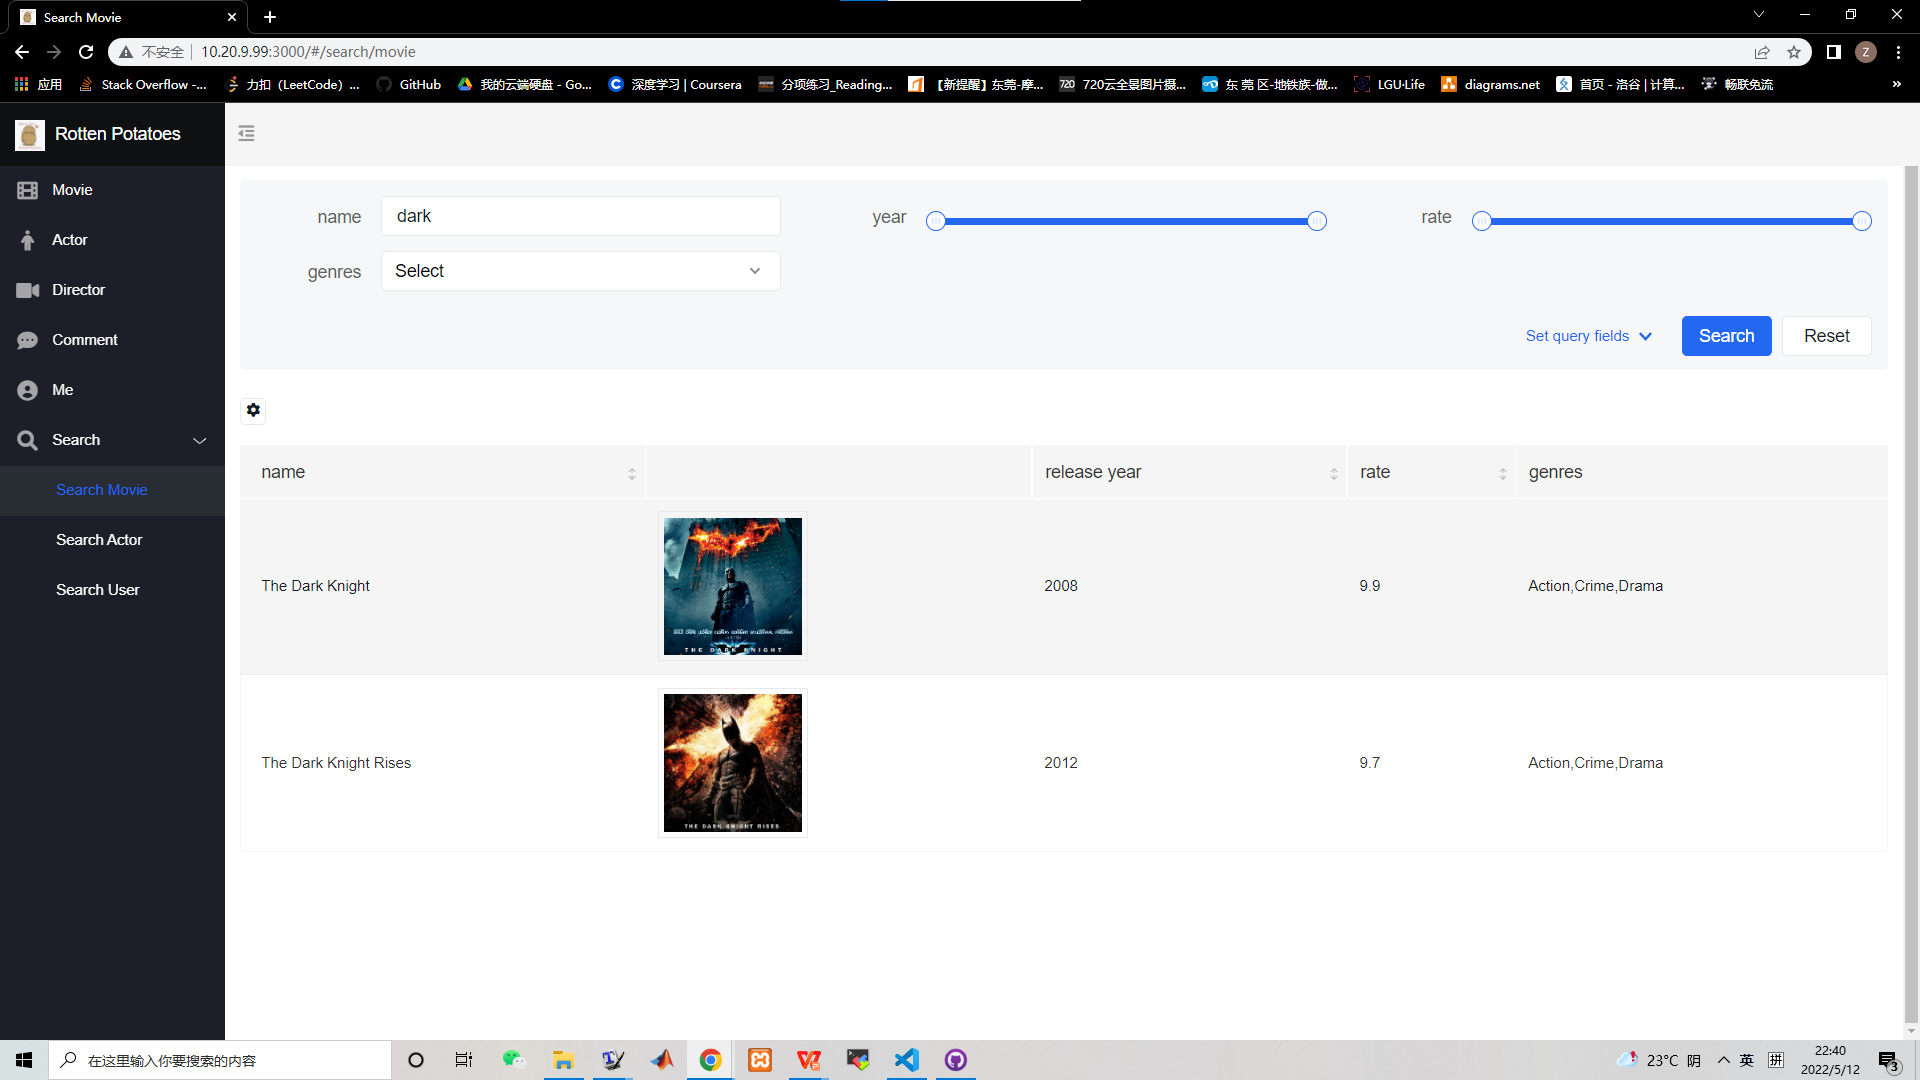
\includegraphics[width=1\textwidth]{res_search2.png}
    \caption{Search movie by name}
    \end{figure}
    
    \begin{figure}[htbp]
    \centering
    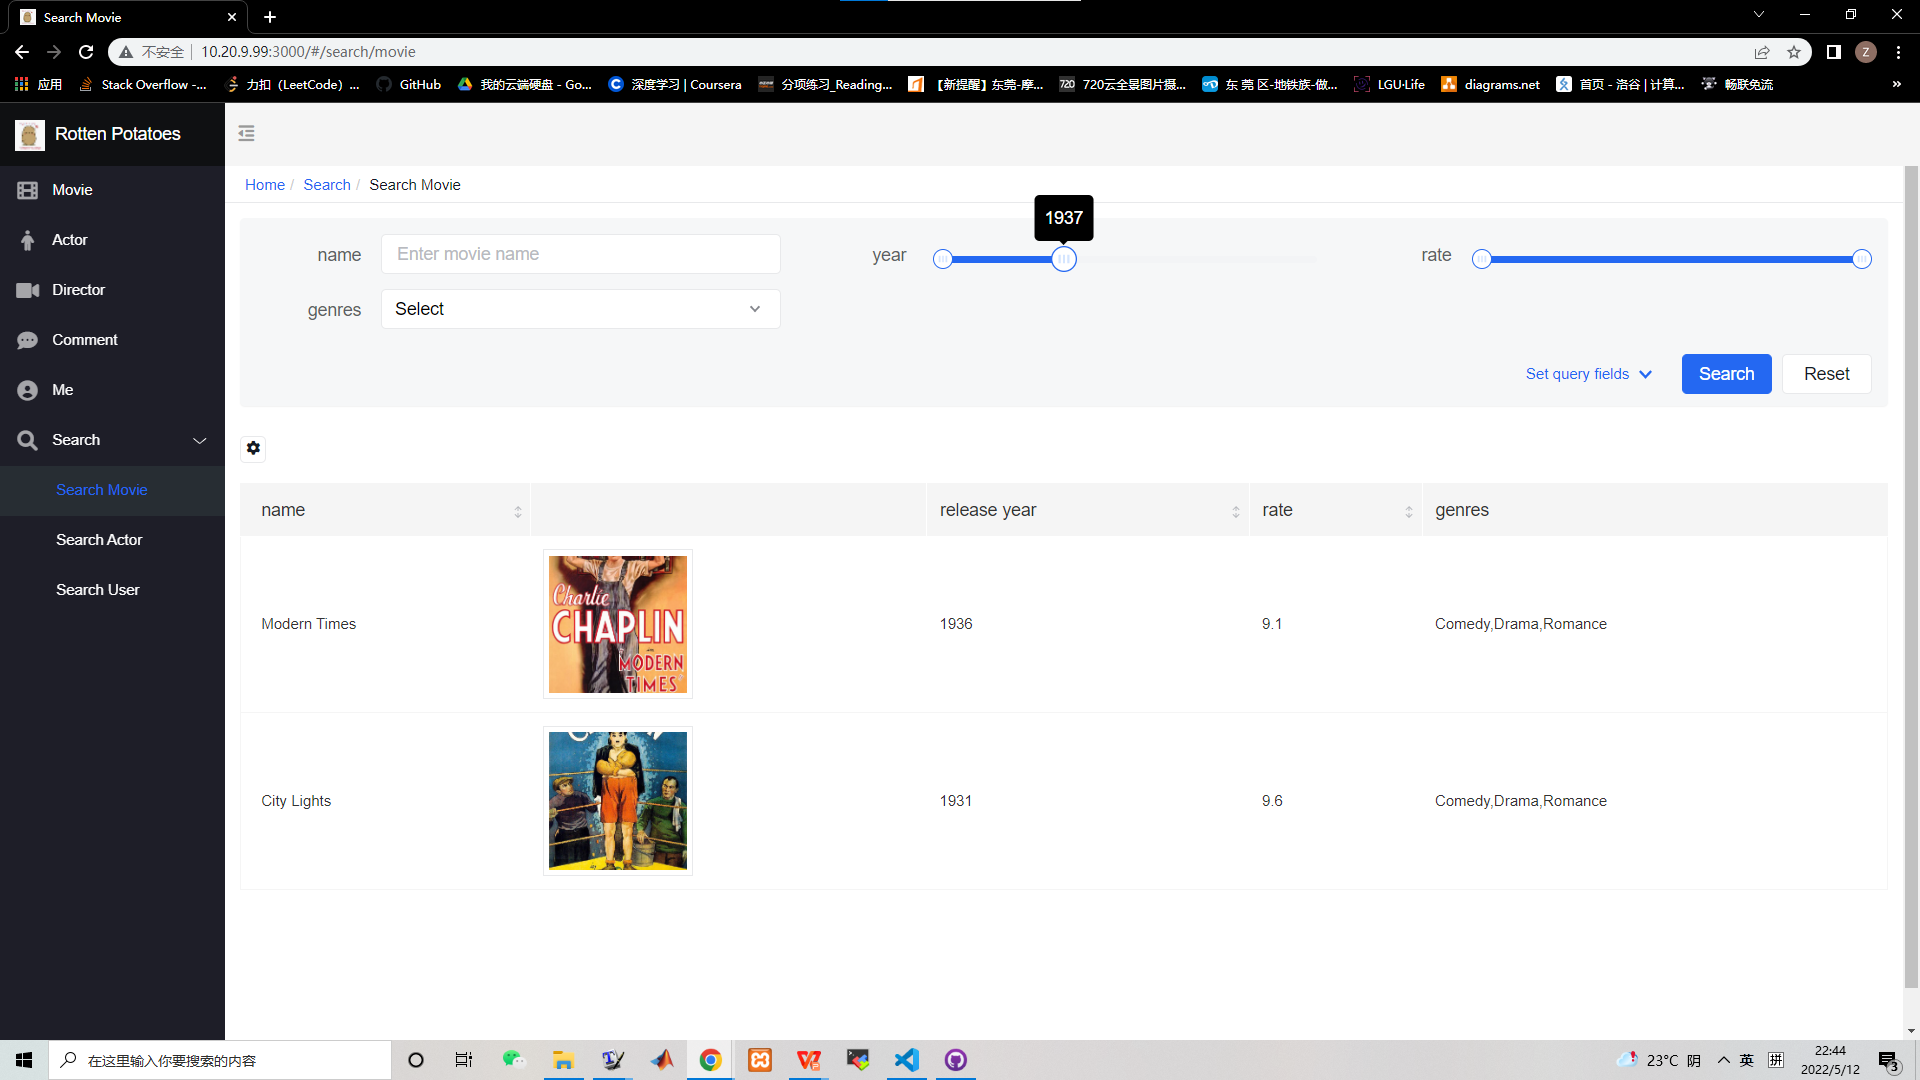
\includegraphics[width=1\textwidth]{res_search3.png}
    \caption{Filter movie by release date}
    \end{figure}
    
    \begin{figure}[htbp]
    \centering
    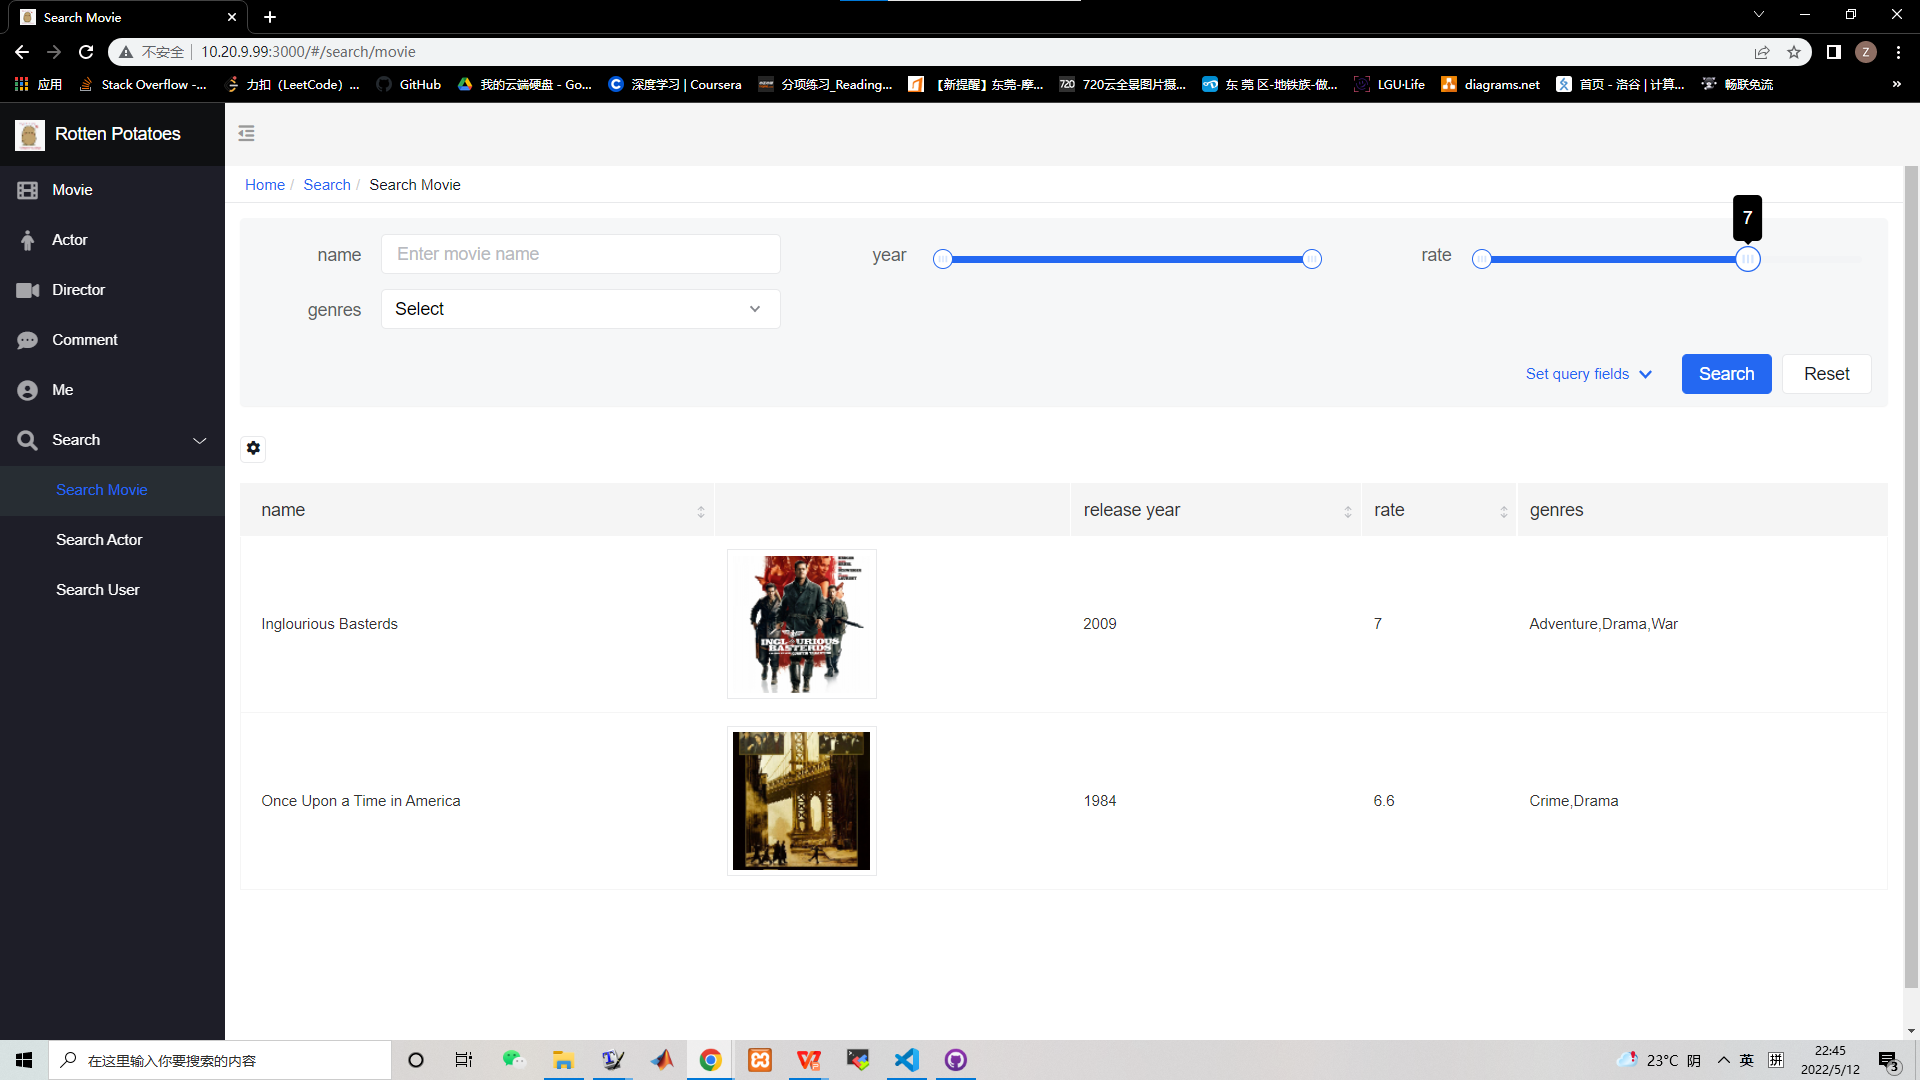
\includegraphics[width=1\textwidth]{res_search4.png}
    \caption{Filter movie by rate}
    \end{figure}
    
    \begin{figure}[htbp]
    \centering
    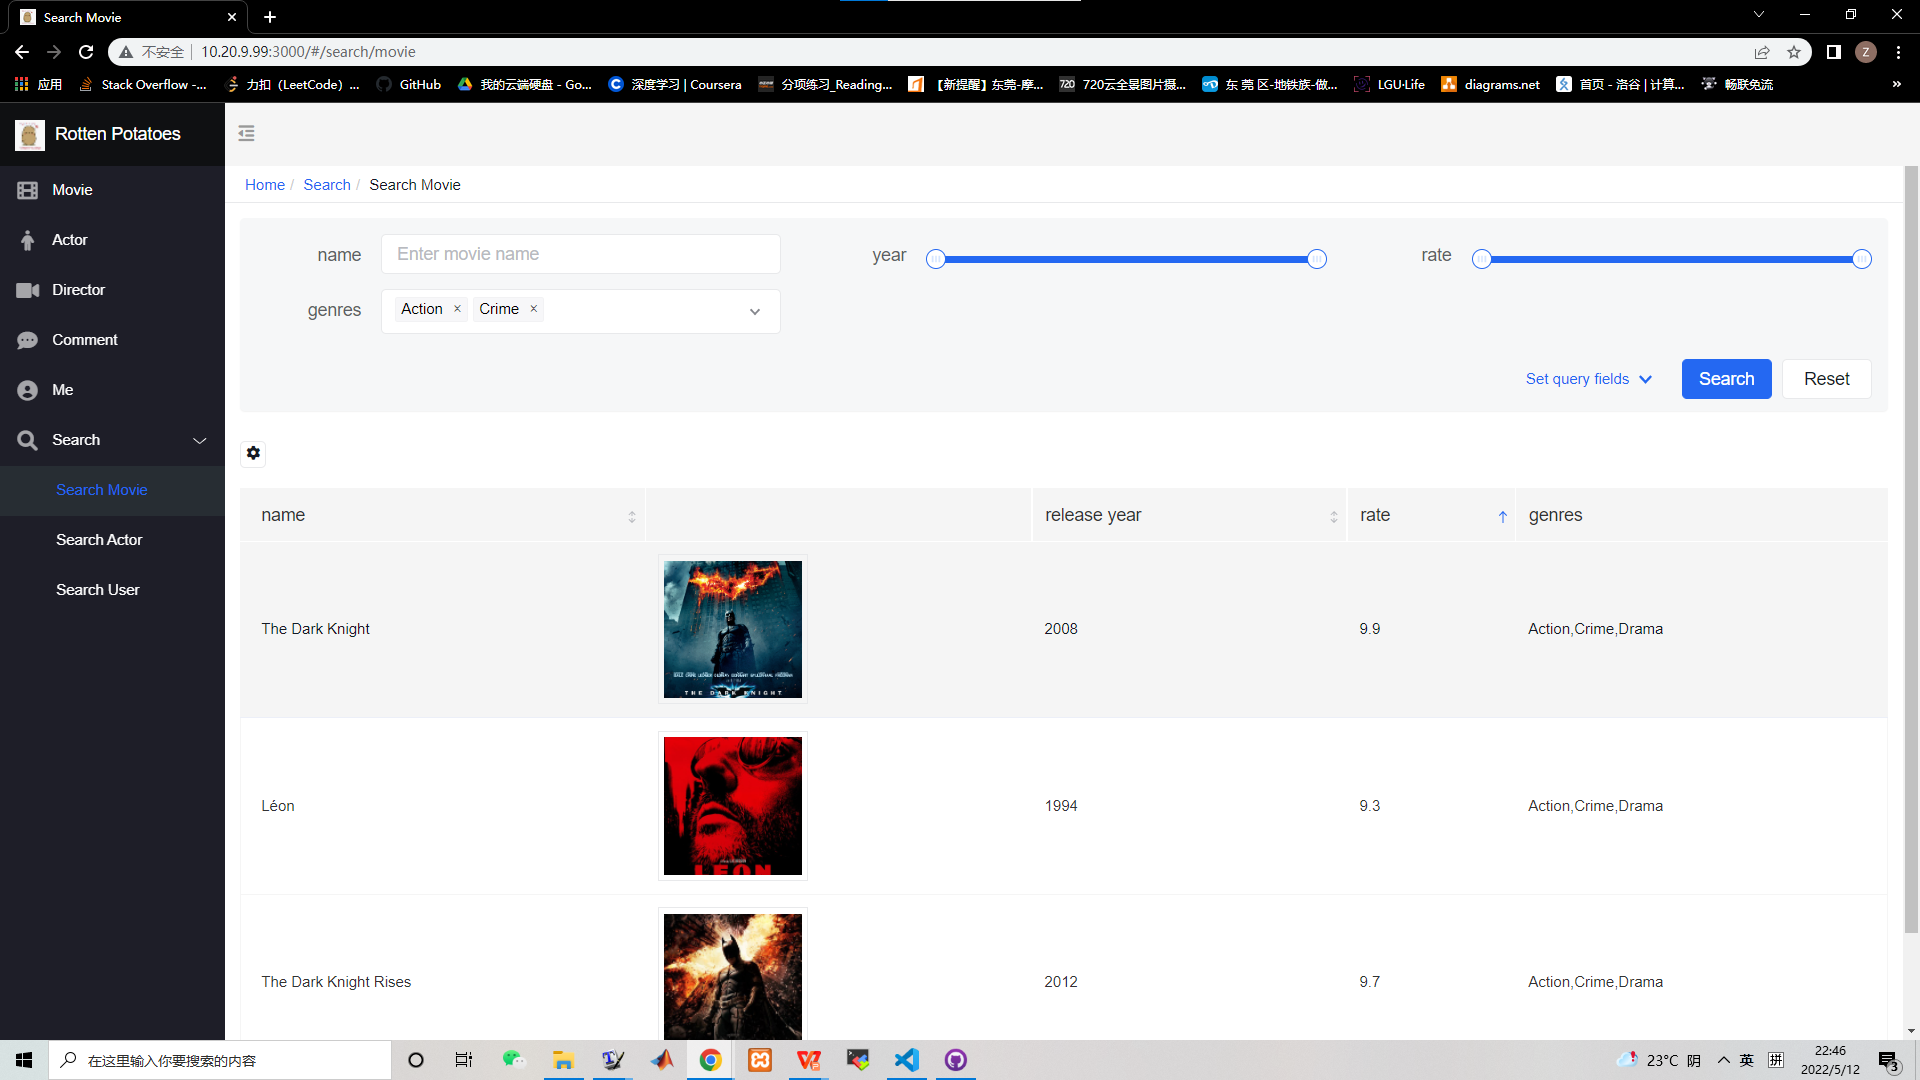
\includegraphics[width=1\textwidth]{res_search5.png}
    \caption{Filter movie by genres}
    \end{figure}
    
    \begin{figure}[htbp]
    \centering
    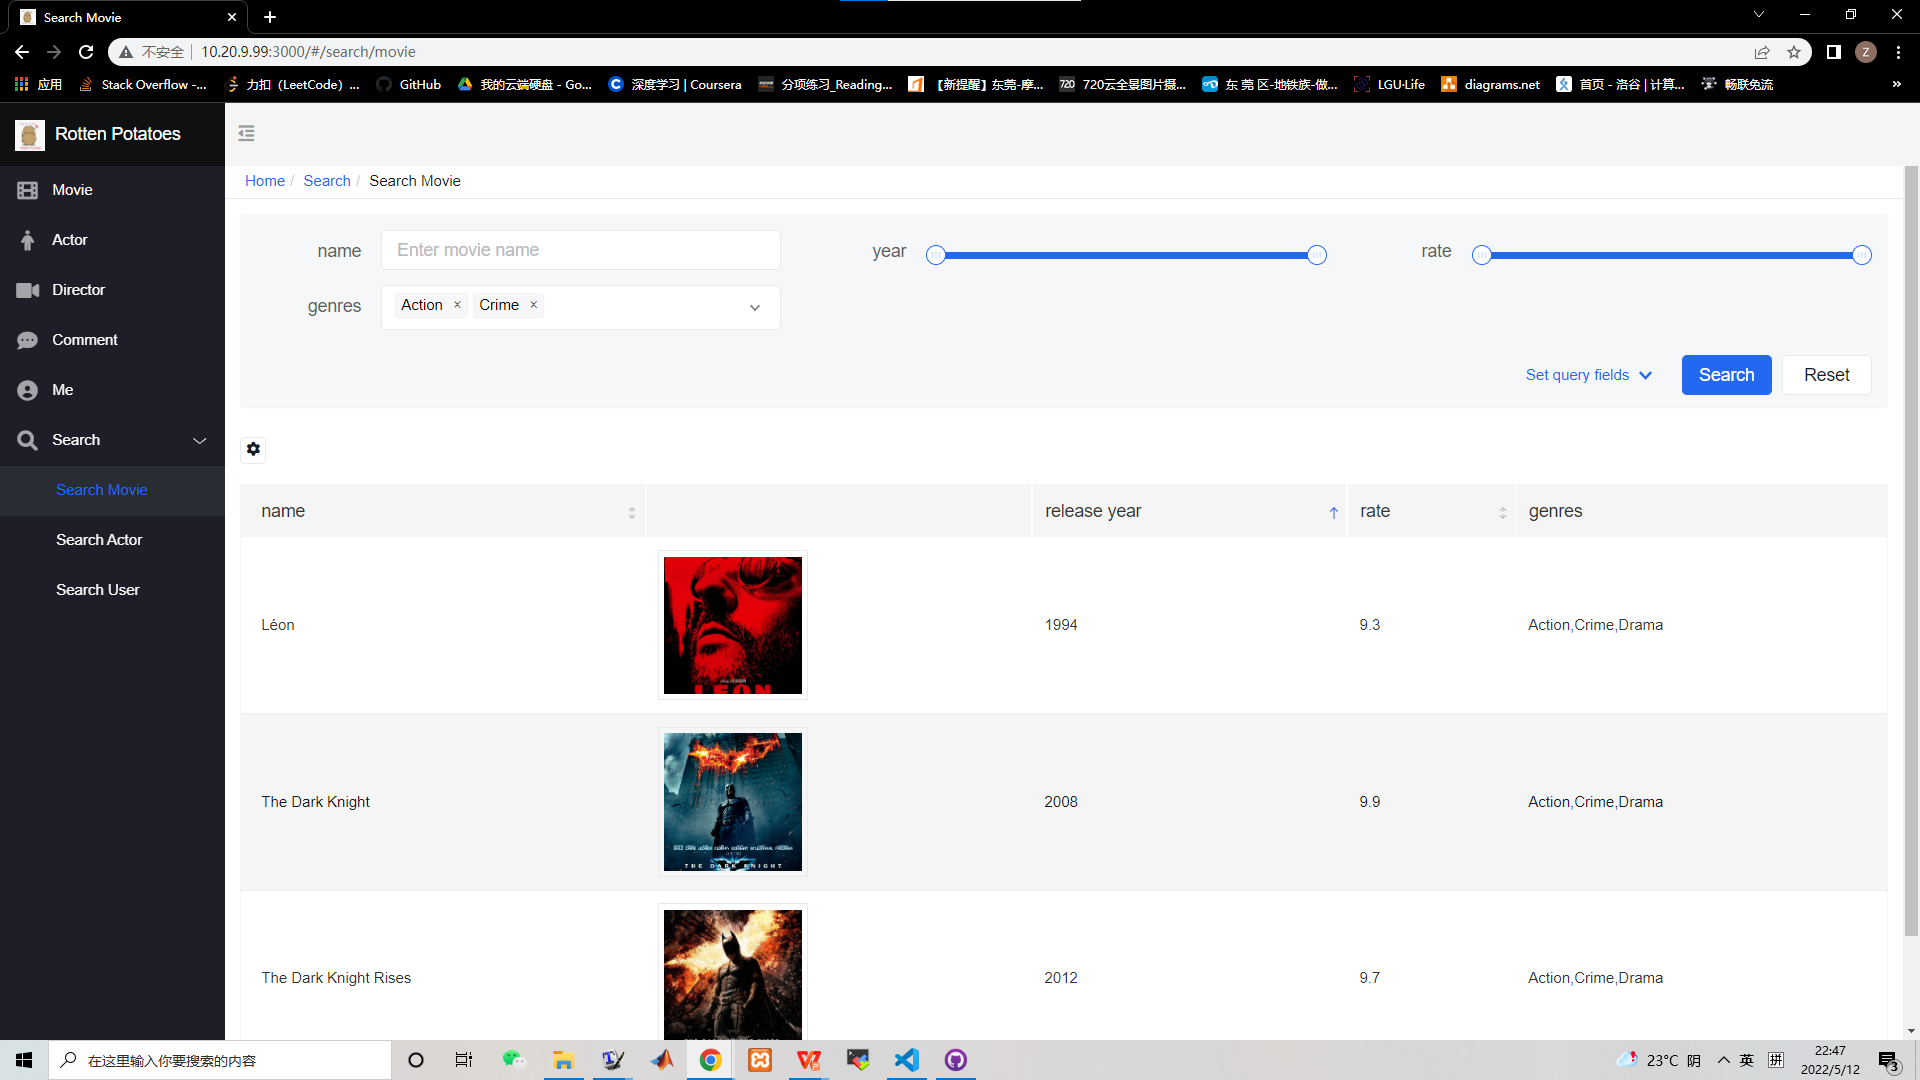
\includegraphics[width=1\textwidth]{res_search6.png}
    \caption{Order movie by release date}
    \end{figure}
    
    \begin{figure}[htbp]
    \centering
    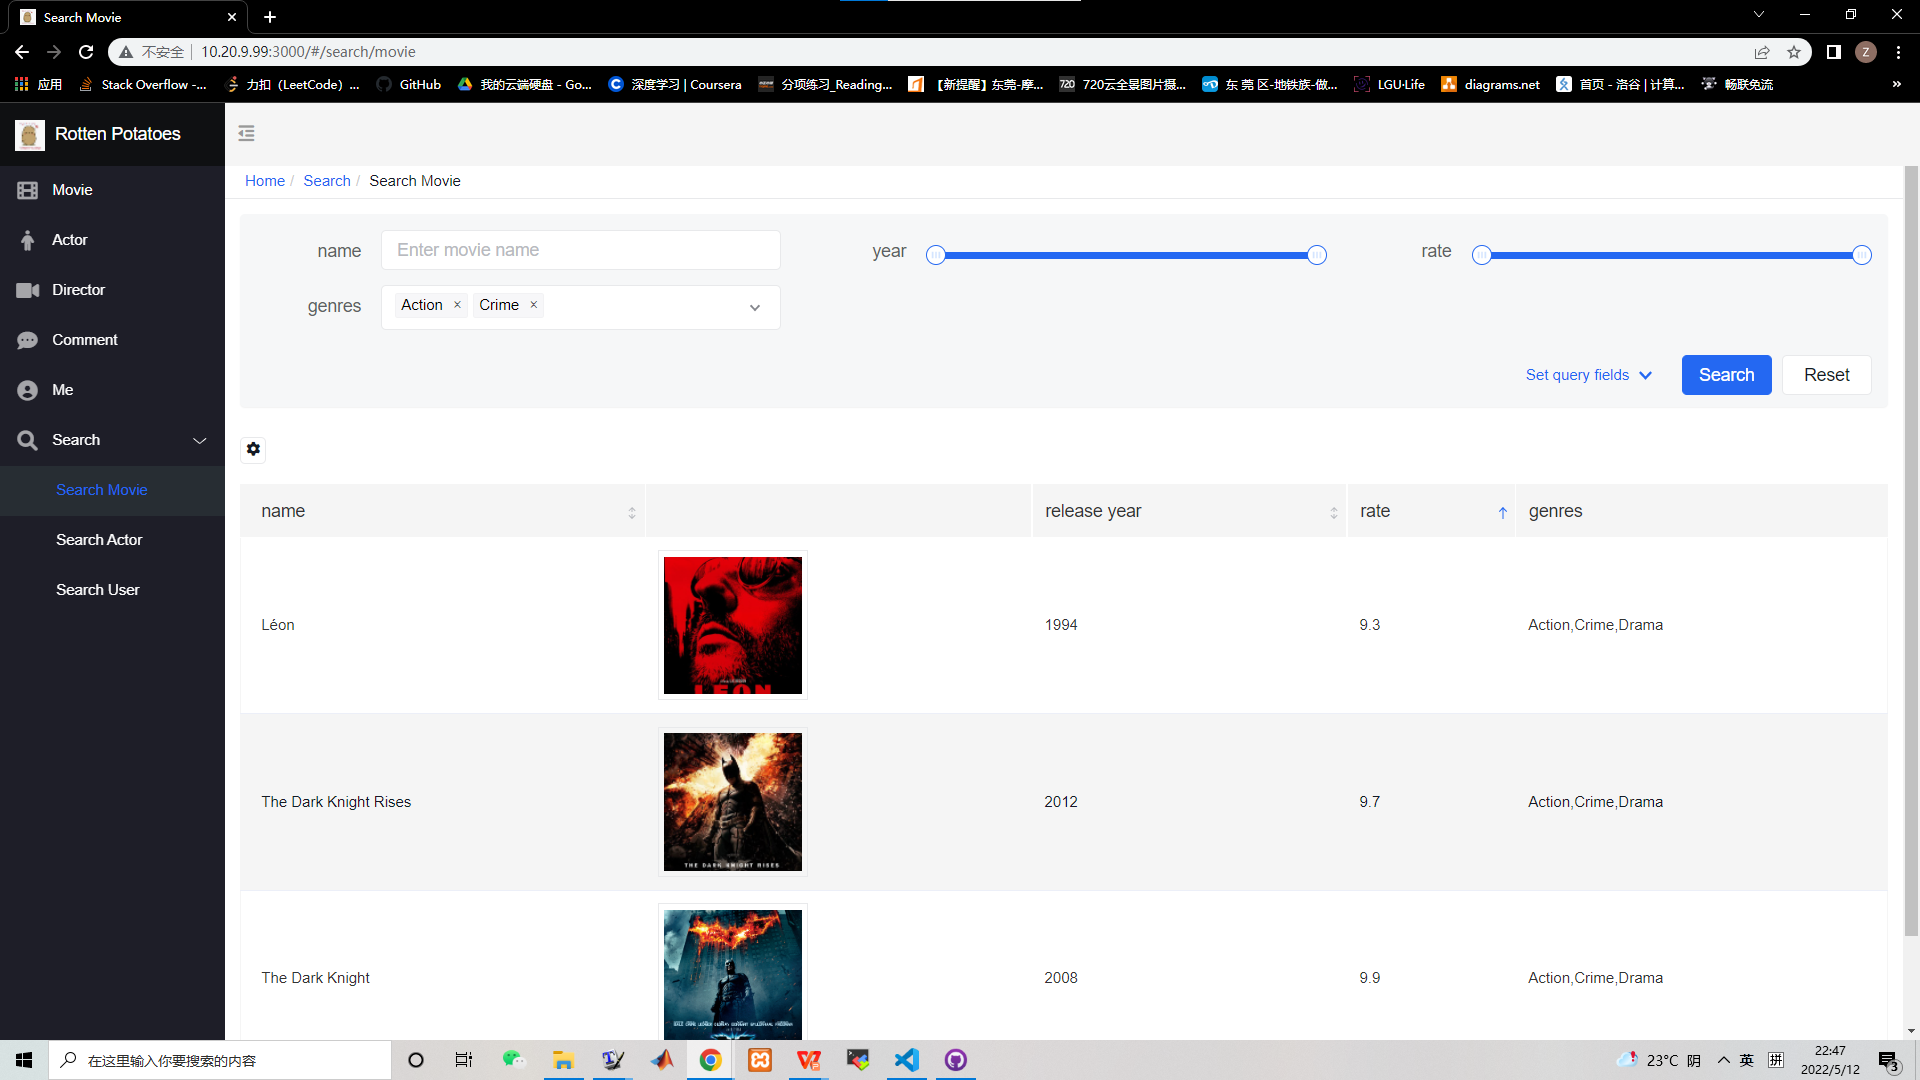
\includegraphics[width=1\textwidth]{res_search7.png}
    \caption{Order movie by rate}
    \end{figure}
    
    \begin{figure}[htbp]
    \centering
    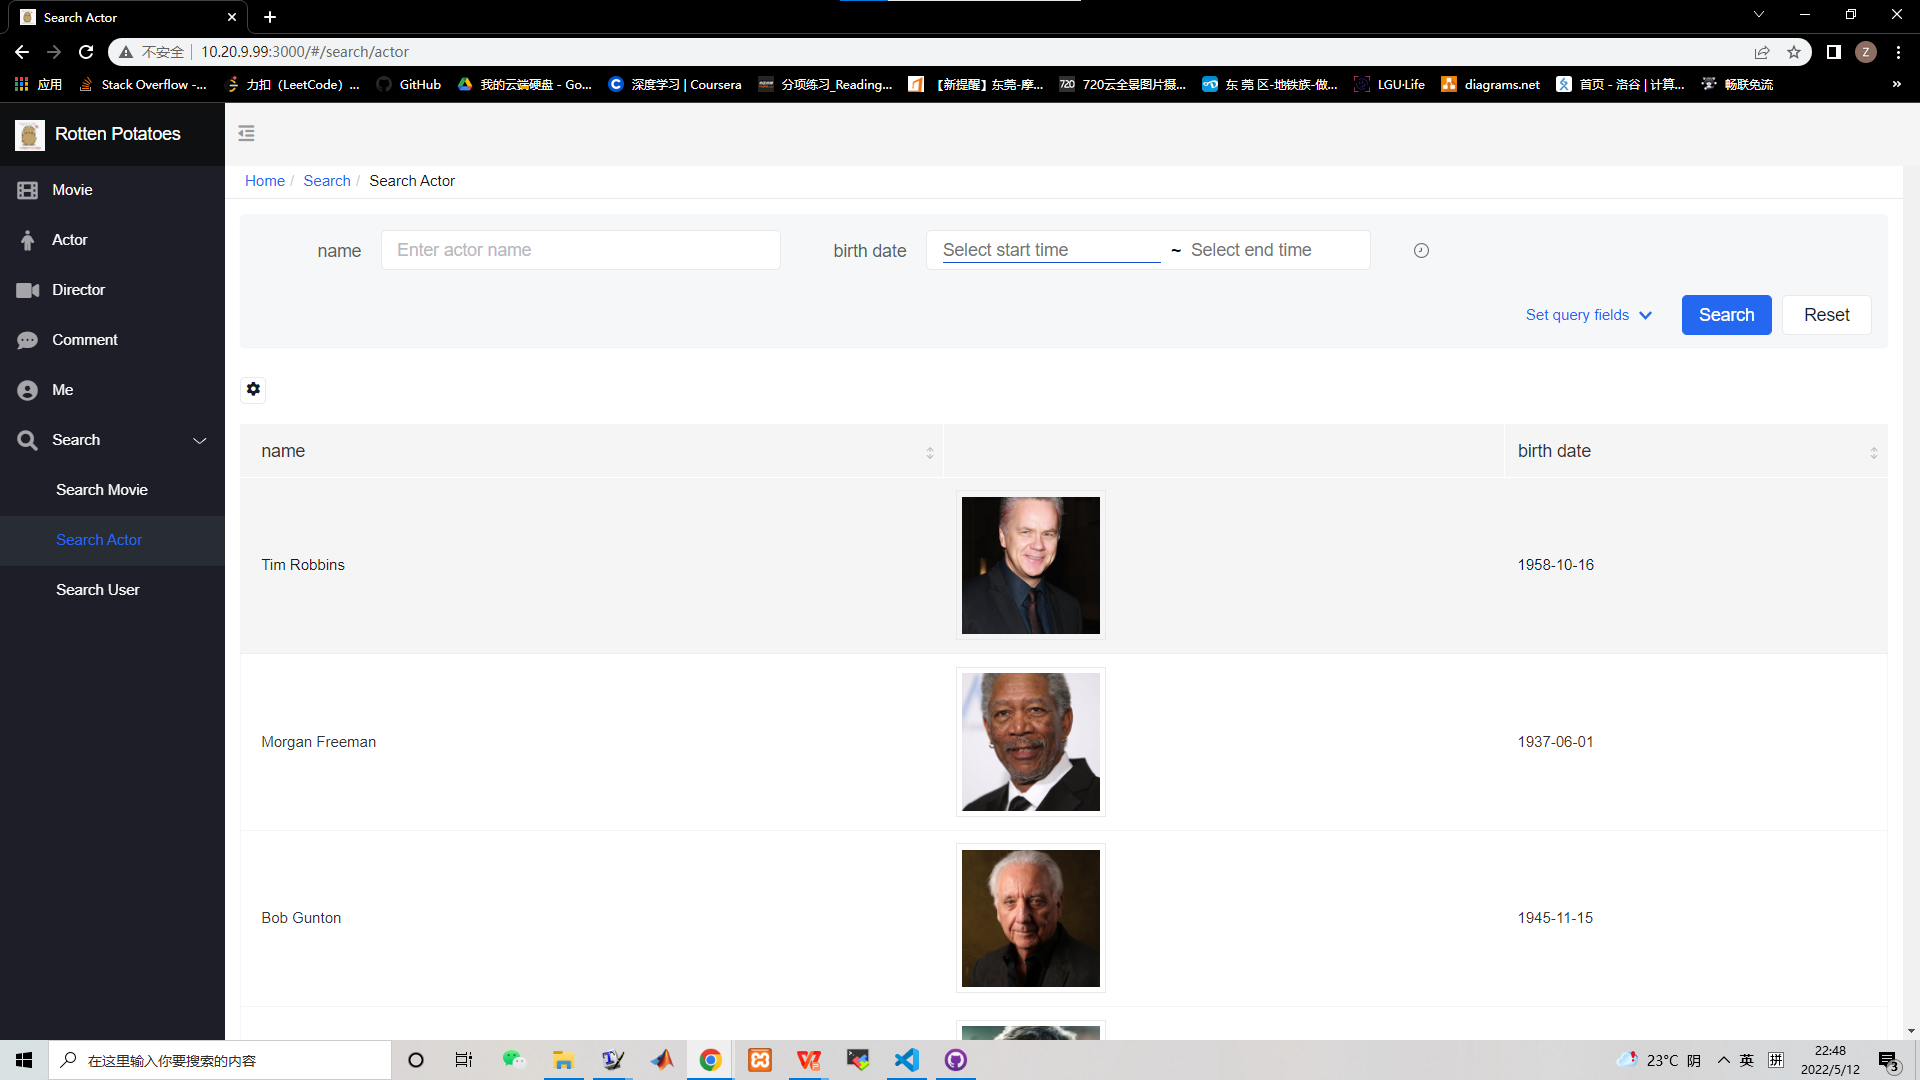
\includegraphics[width=1\textwidth]{res_search8.png}
    \caption{Actor search page}
    \end{figure}
    
    \begin{figure}[htbp]
    \centering
    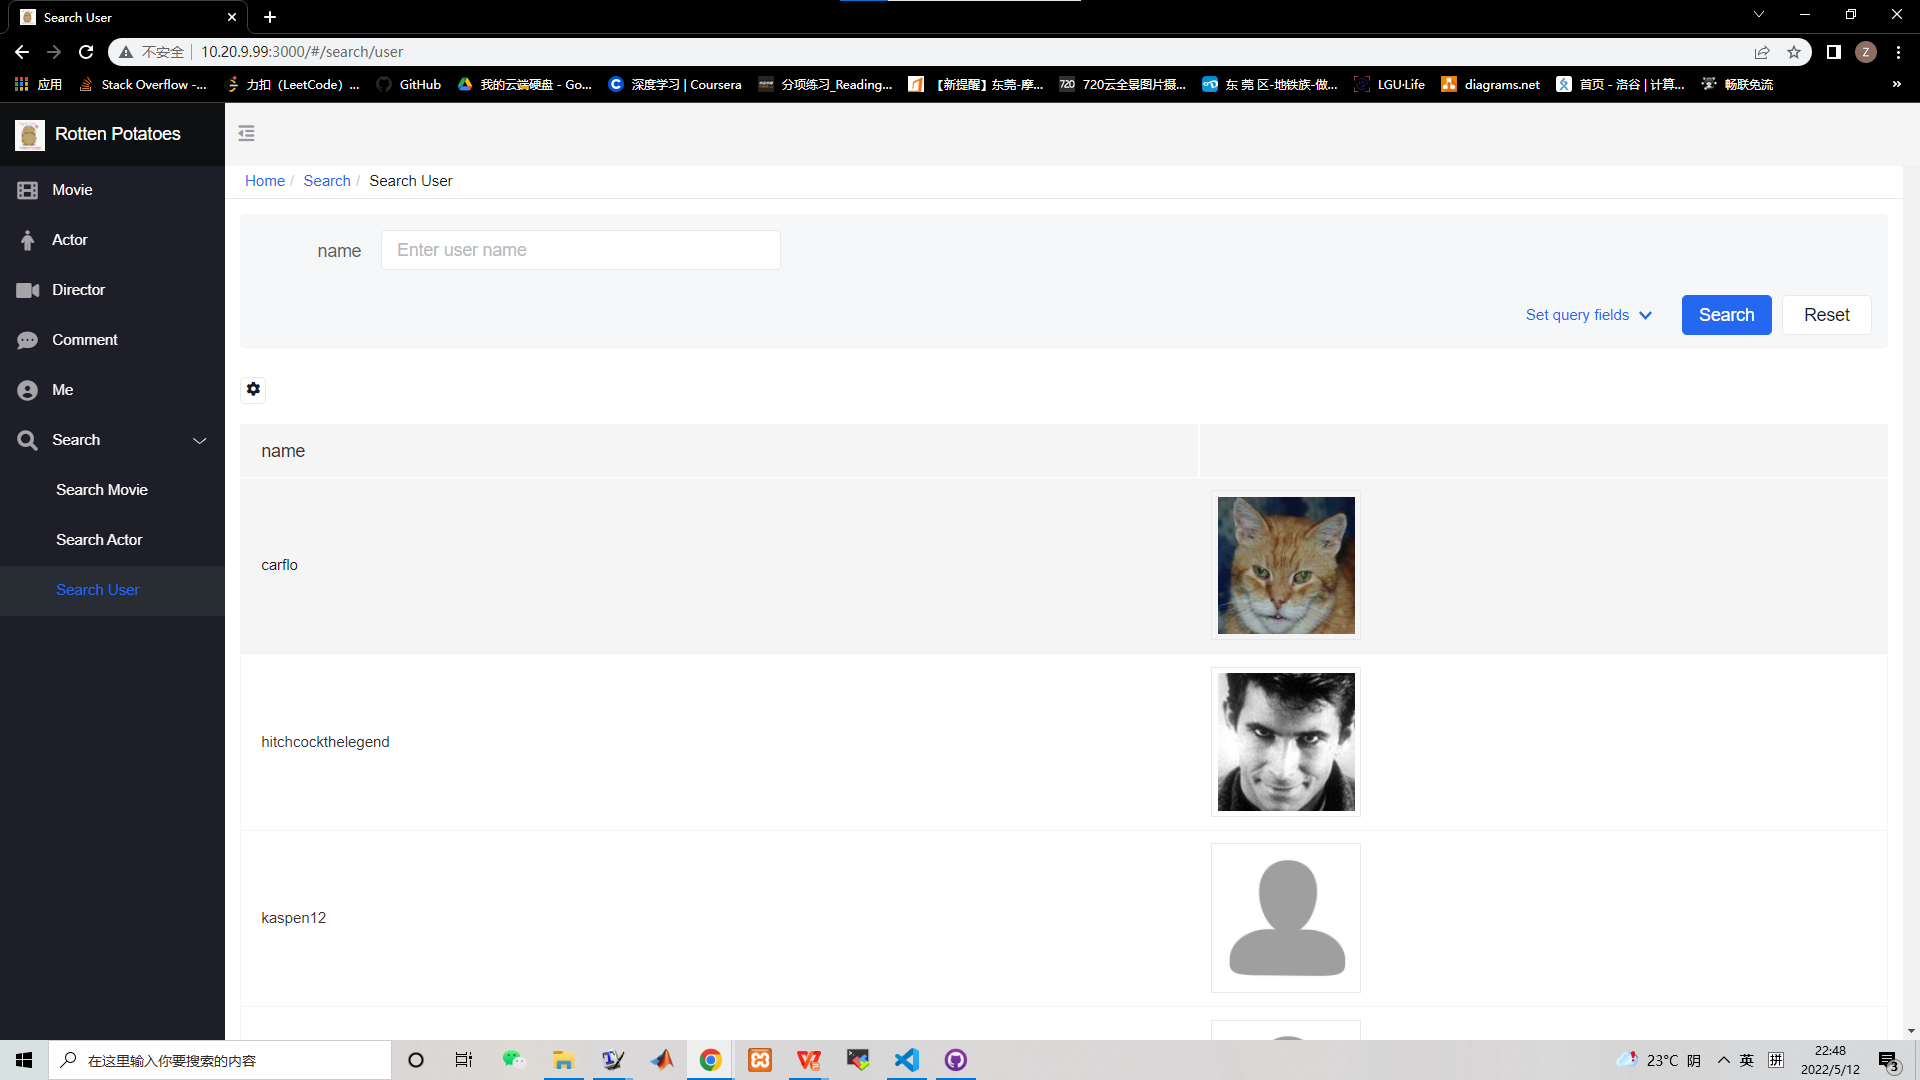
\includegraphics[width=1\textwidth]{res_search9.png}
    \caption{User search page}
    \end{figure}
    
    \begin{figure}[htbp]
    \centering
    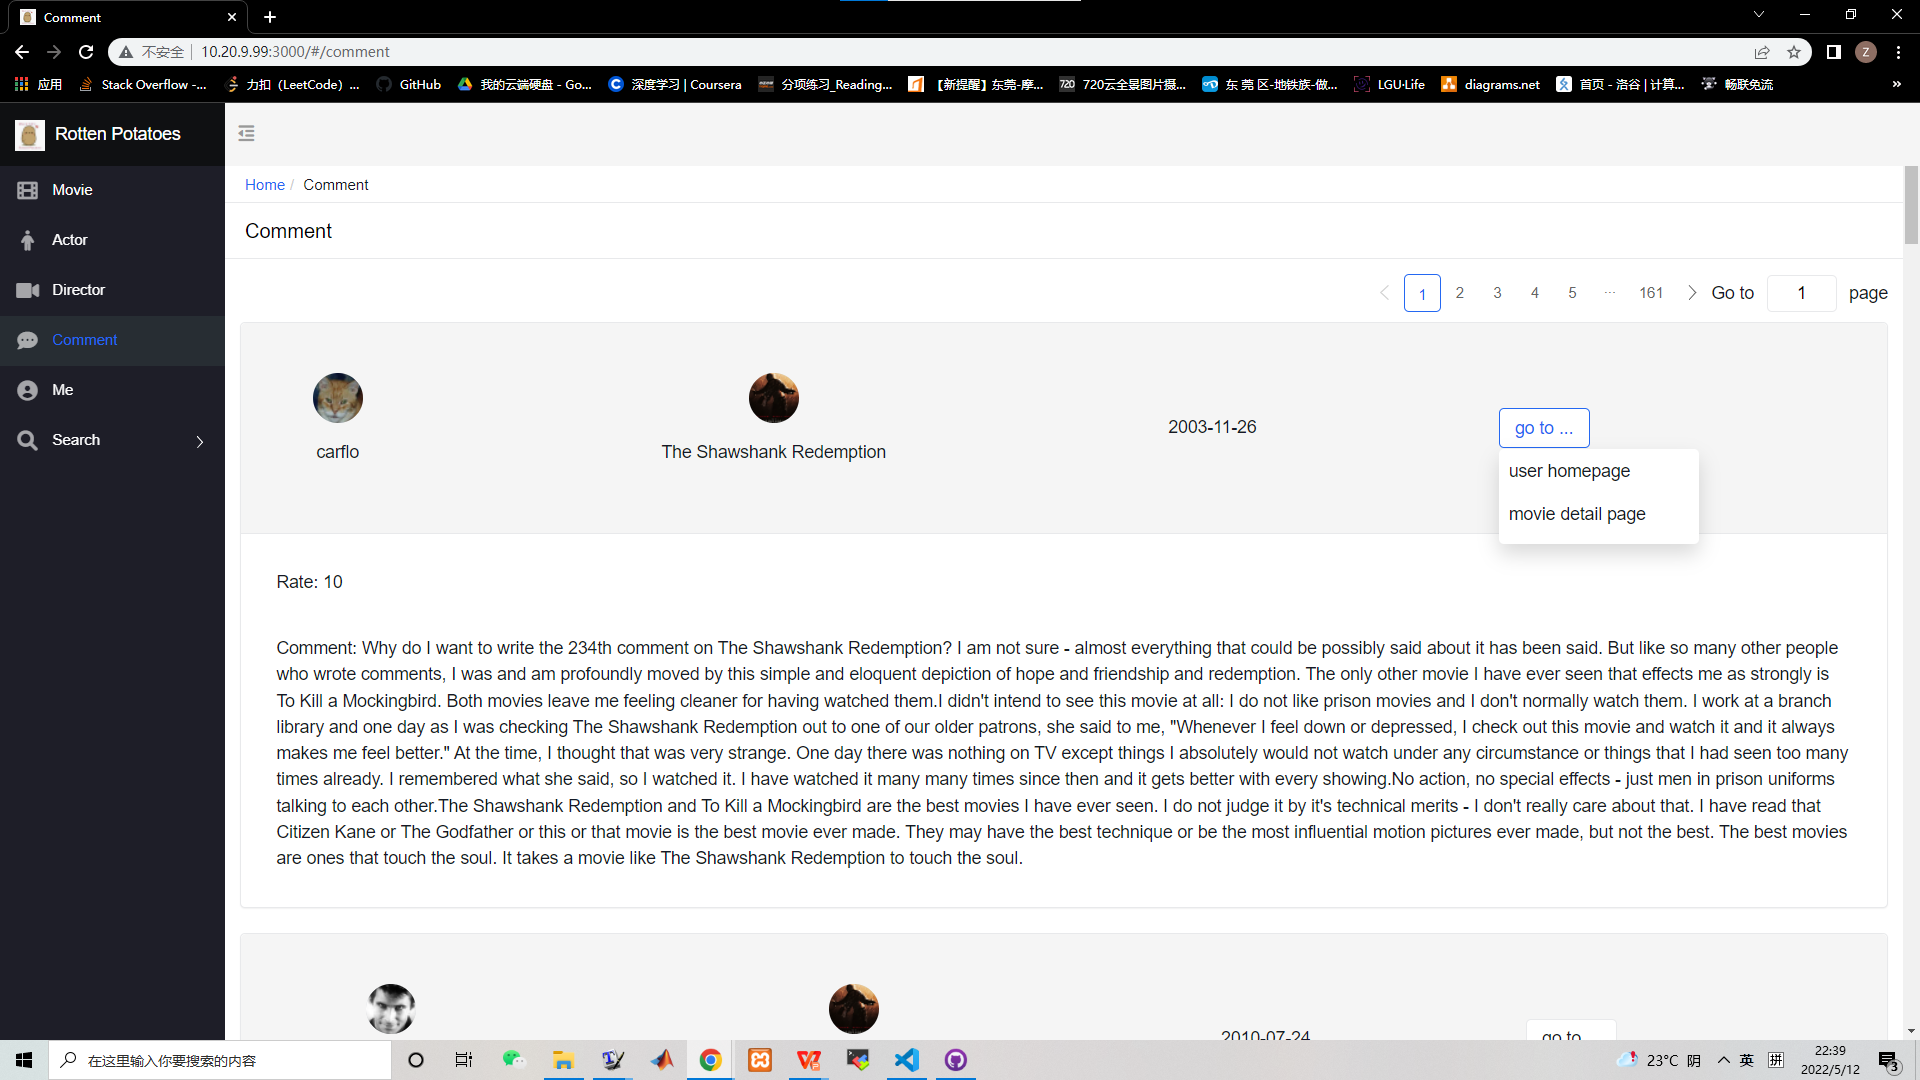
\includegraphics[width=1\textwidth]{res_comment1.png}
    \caption{Comment list}
    \end{figure}
    
    \begin{figure}[htbp]
    \centering
    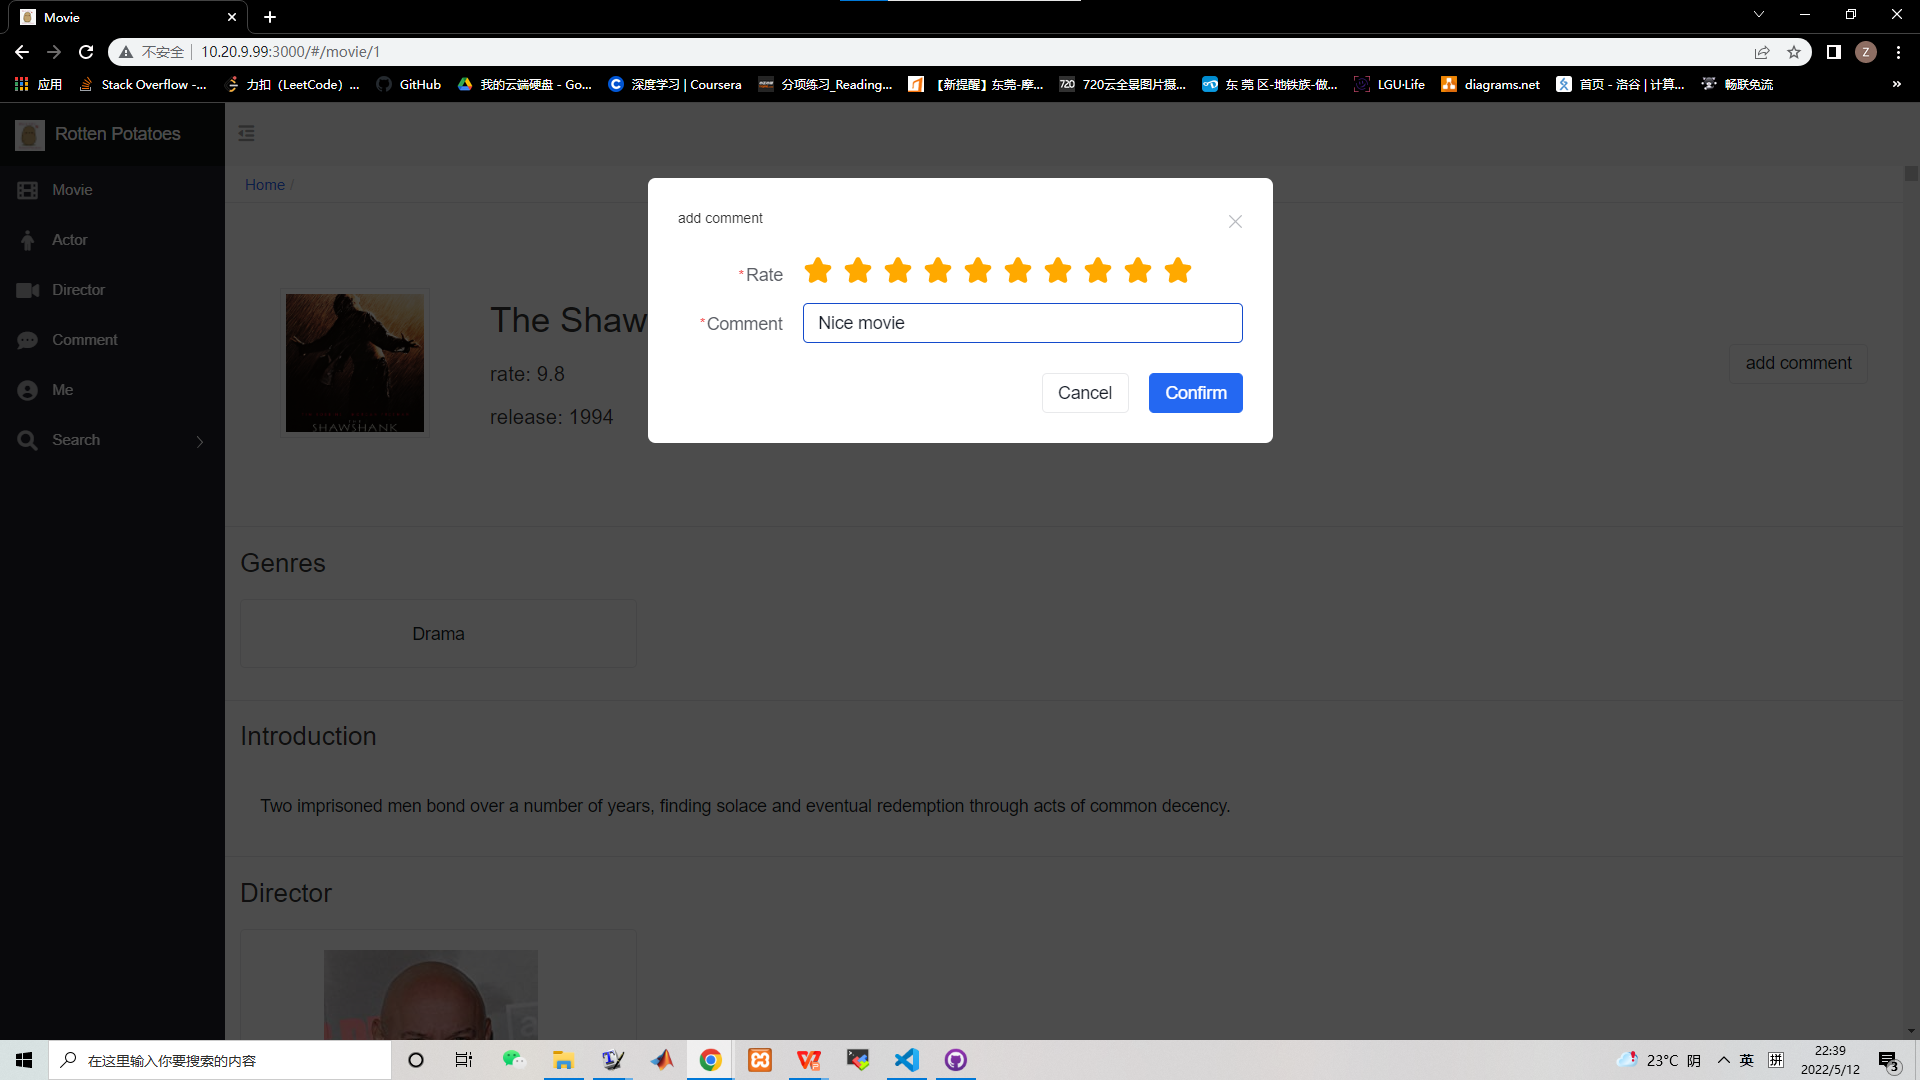
\includegraphics[width=1\textwidth]{res_comment2.png}
    \caption{Add comment}
    \end{figure}
    
    \begin{figure}[htbp]
    \centering
    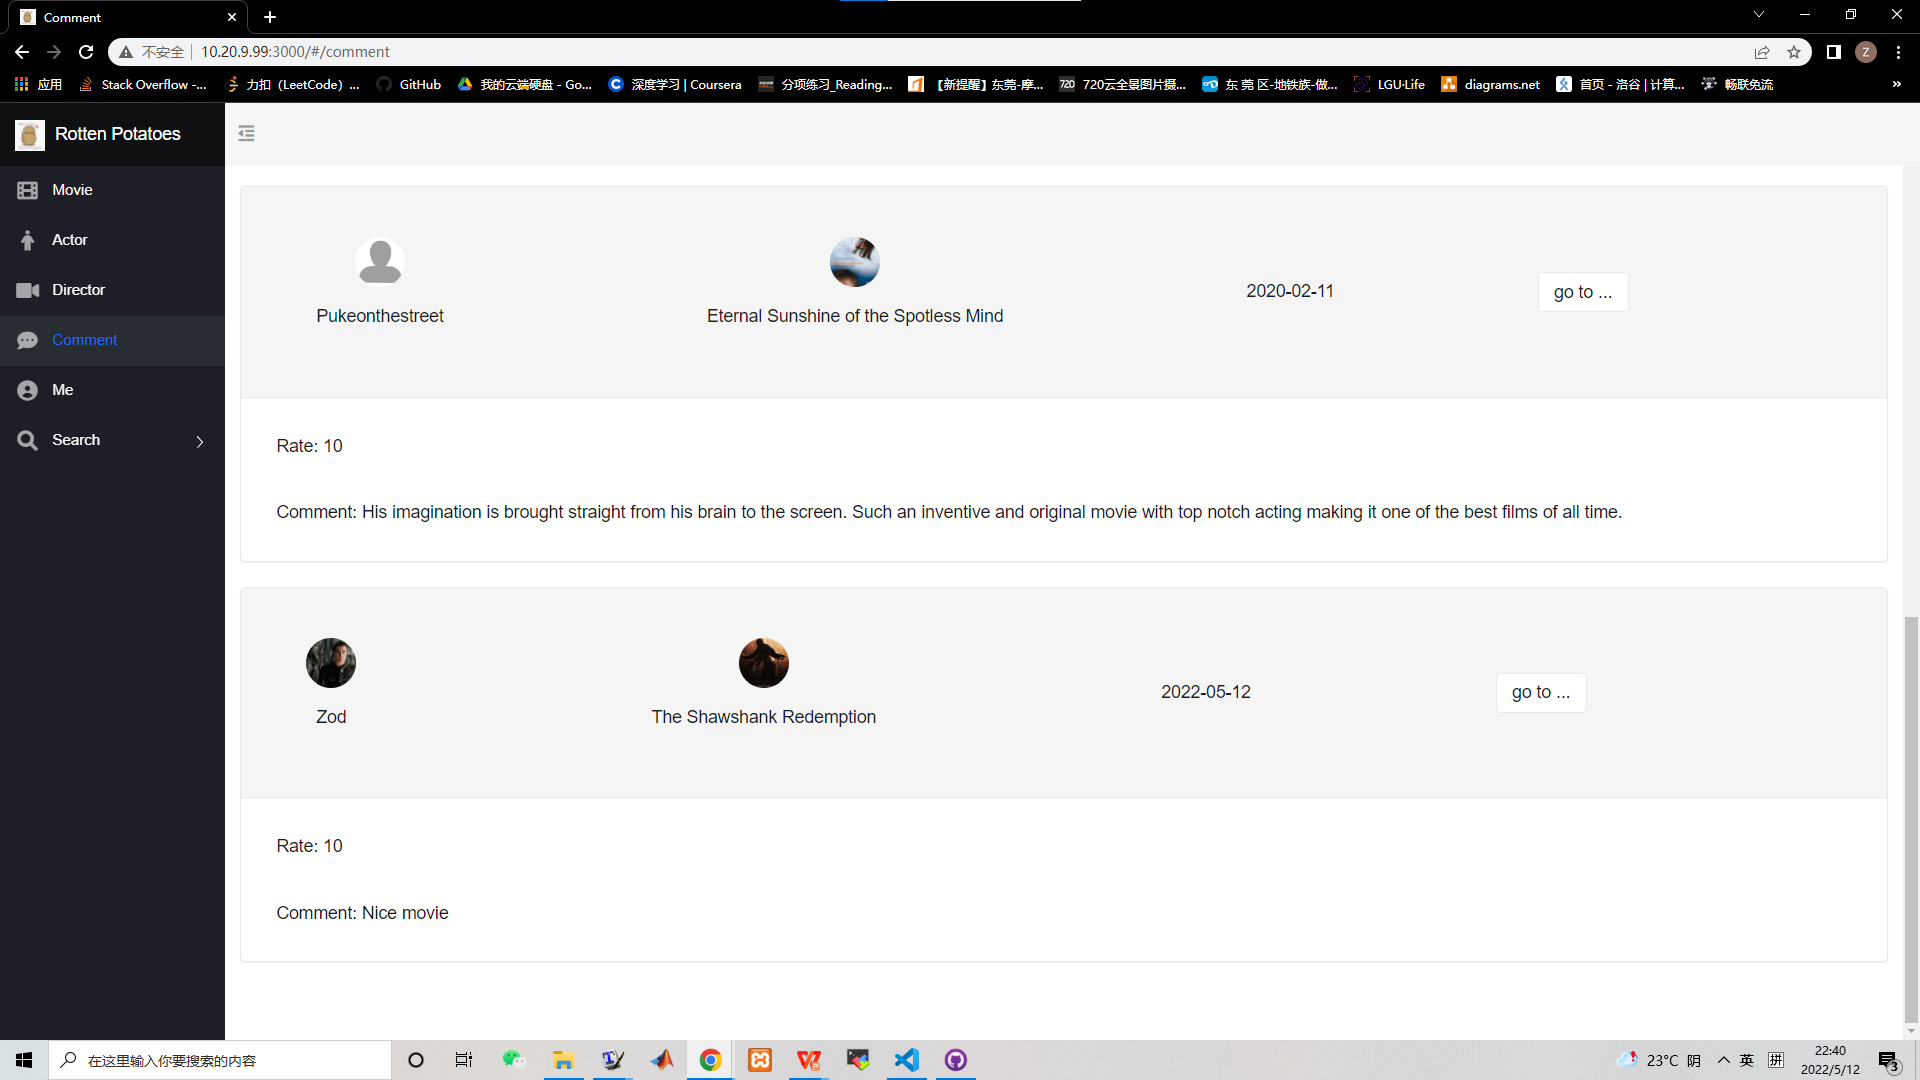
\includegraphics[width=1\textwidth]{res_comment3.png}
    \caption{Comment before deleting user account}
    \end{figure}
    
    \begin{figure}[htbp]
    \centering
    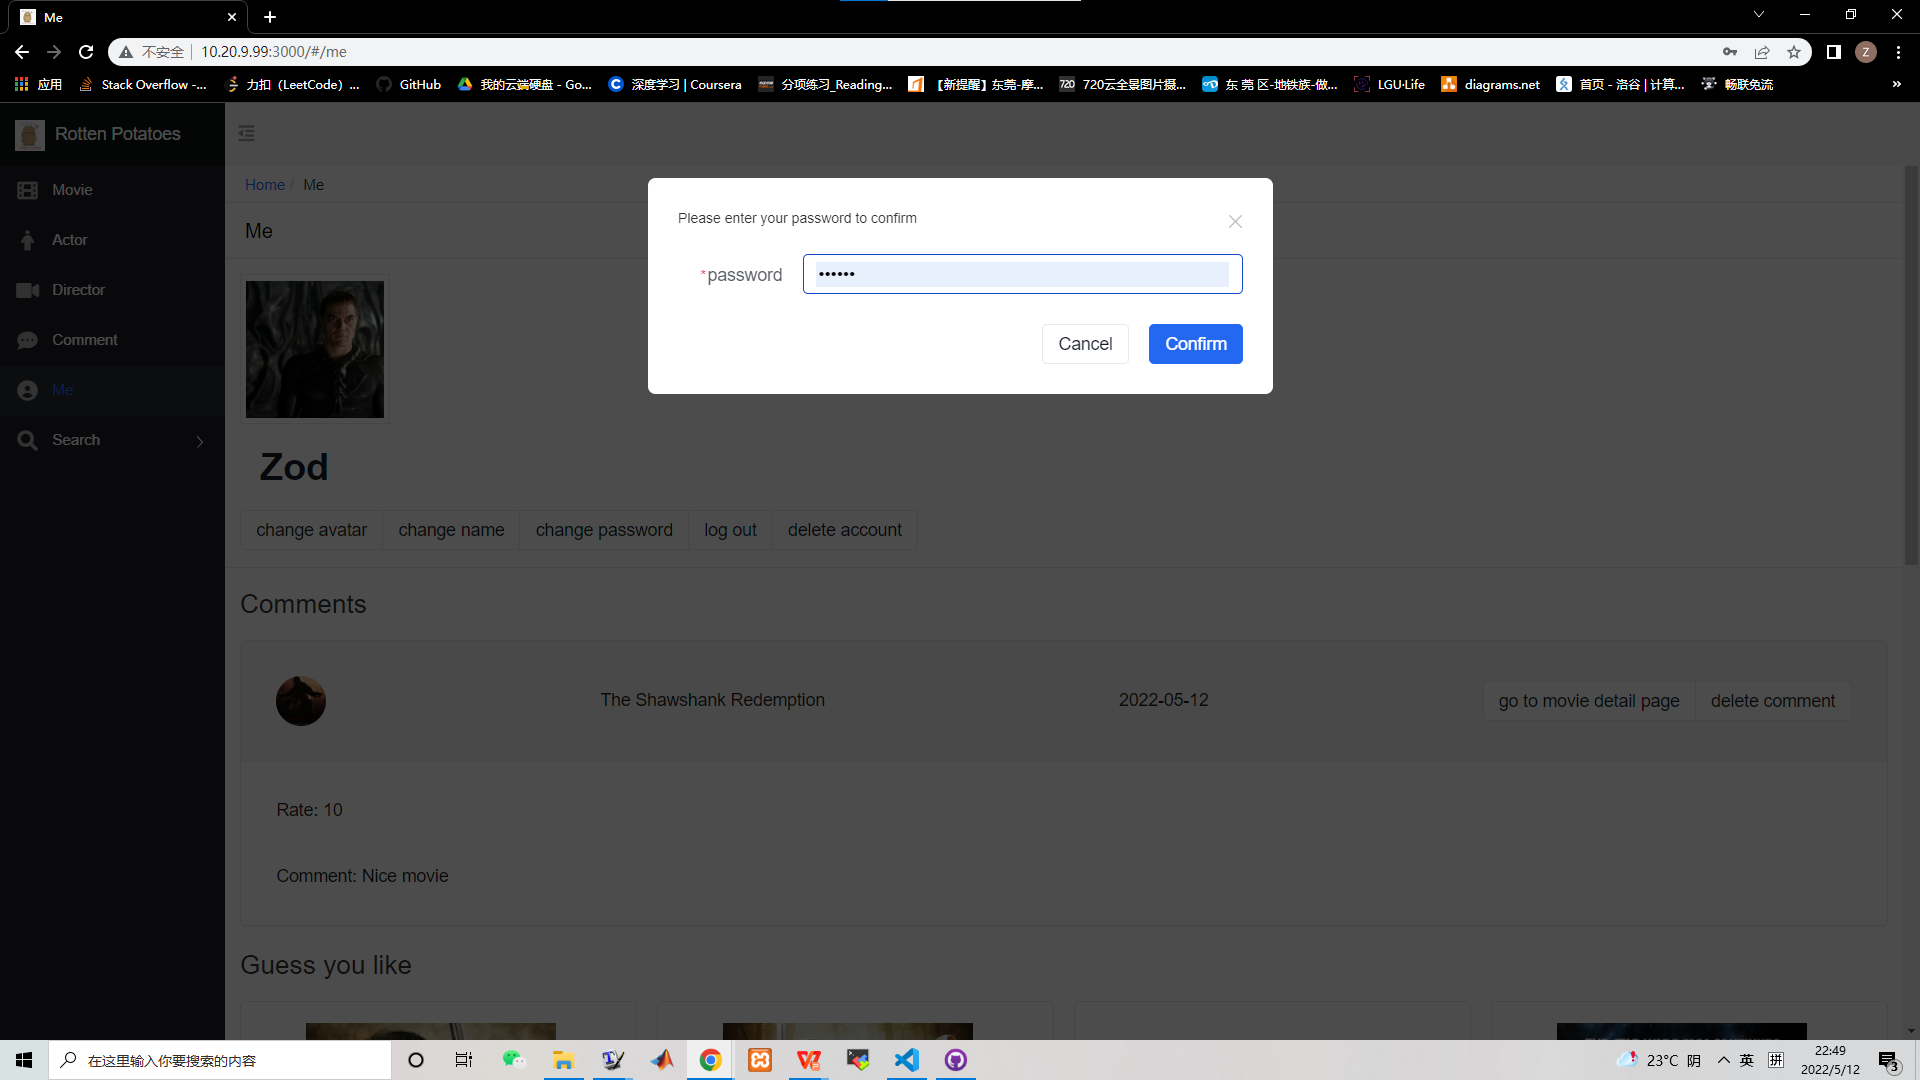
\includegraphics[width=1\textwidth]{res_delete1.png}
    \caption{Delete user account}
    \end{figure}
    
    \begin{figure}[htbp]
    \centering
    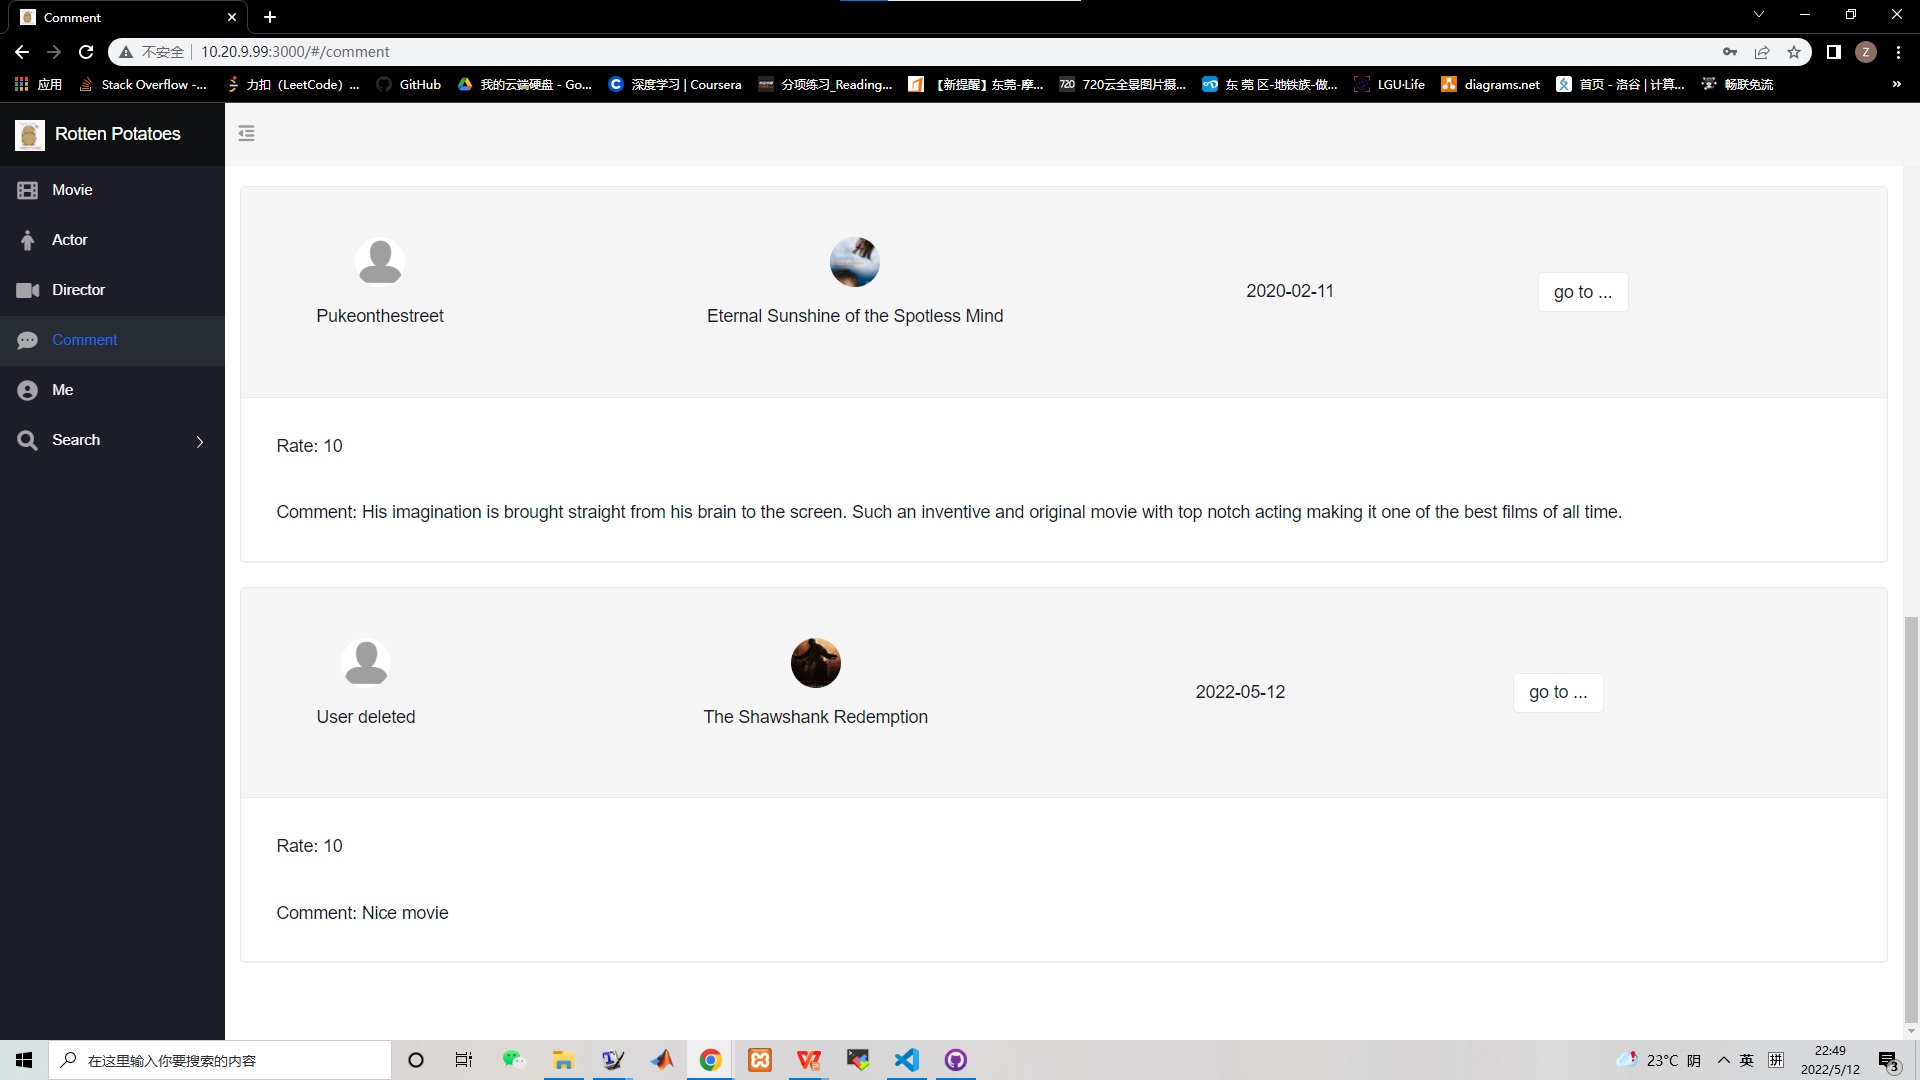
\includegraphics[width=1\textwidth]{res_delete2.png}
    \caption{Comment after deleting user account}
    \end{figure}
\end{CJK*}
\end{document}
